\documentclass[10pt]{book}
\usepackage[utf8]{inputenc}
\usepackage[italian]{babel}
\usepackage{multicol}
\usepackage[bookmarks]{hyperref}
\usepackage[a4paper, total={18cm, 25cm}]{geometry}
\usepackage{tikz}
\usepackage{color}
\usepackage{relsize}
\usepackage{amsmath}
\usepackage{amsfonts}
\definecolor{mygray}{rgb}{0.5,0.5,0.5}
\usepackage{listings}
\usepackage{mathrsfs}
\lstset{
	language=Matlab,
	commentstyle=\color{mygray}
}
\usepackage{graphicx}
\usepackage{makecell}
\graphicspath{ {./img/} }
\usepackage{color}

\begin{document}
\renewcommand*\contentsname{Indice}
\title{Calcolo Numerico}
\author{Federico Matteoni}
\date{A.A. 2019/20}
\maketitle
\tableofcontents
\pagebreak
\section*{Introduzione}
Prof.: Luca Gemignani
\paragraph{Calcolo Numerico} Metodi numerici per risolvere problemi matematici con il calcolatore. In questo corso ce ne occuperemo dal punto di vista numerico, perché metodi di risoluzione diversi performano in maniera diversa sulla macchina. Cerchiamo di capire quali sono i metodi di interesse e cosa aspettarci dalla loro implementazione.\\
Il \textbf{metodi numerici approssimano la soluzione di problemi matematici}.\\
Inoltre, il computer \textbf{impatta} sul calcolo perché lavora con approssimazioni dei numeri, che su moli elevate di dati e di elaborazioni finiscono per perturbare il risultato ottenuto.
\paragraph{Programma 2019/20} \begin{verbatim}
2 L'Aritmetica del Calcolatore
Lezione 2.1:Rappresentazione in Base e Numeri di Macchina.
Lezione 2.2:Aritmetica di Macchina (Teorema 2.2.1).


3 Analisi degli Errori
Lezione 3.1:Errori nel Calcolo di una Funzione Razionale (Teorema 3.1.1)
Lezione 3.2:Tecniche per l'Analisi degli Errori (senza analisi all'indietro).
Lezione 3.3:Cenni sul Calcolo di una Funzione non Razionale.


4 I Problemi dell'Algebra Lineare Numerica:Aspetti Computazionali e Condizionamento
Lezione 4.1:Norme Matriciali e Norme Vettoriali.
Lezione 4.2:Il Problema della Risoluzione di un Sistema Lineare ed il
suo Condizionamento.
Lezione 4.3:Il Problema del Calcolo degli Autovalori di una Matrice
Lezione 4.4:Teoremi di Localizzazione per Autovalori (Teorema 4.4.1).

5 Metodi Diretti per la Risoluzione di Sistemi Lineari
Lezione 5.1:Sistemi Triangolari (Teorema 5.1.1)
Lezione 5.2:Matrici Elementari di Gauss ed il Metodo di Eliminazione
Gaussiana
Lezione 5.3:Il Metodo di Gauss per Matrici Invertibili: Tecniche di
Pivoting e Stabilita`.

6 Metodi Iterativi per la Risoluzione di Sistemi Lineari
Lezione 6.1:Generalita` sui Metodi Iterativi (Teorema 6.1.2, Teorema 6.1.3). 
Lezione 6.2:I Metodi di Jacobi e Gauss-Seidel. 
Lezione 6.3:Convergenza dei Metodi di Jacobi e Gauss-Seidel (Teorema 6.3.1).

9 Alcuni Problemi Numerici in Teoria dell'Approssimazione 70

10 Metodi Numerici per l'Approssimazione degli Zeri di una Funzione
Lezione 10.1: Il Metodo di Bisezione (Teorema 10.1.1;  per informatica con ipotesi  addizionale di
separazione)
Lezione 10.2: Metodi di Iterazione Funzionale (Teorema 10.2.2, Teorema 10.2.3).
Lezione 10.3: Il Metodo delle Tangenti (Teorema 10.3.1)

\end{verbatim}
\paragraph{Tipici problemi} $$Ax = b\:\:\:\:\:Ax = \lambda x$$ $$f(x) = 0\:\:\:\:\:\int_a^bf(x) dx$$
\paragraph{Matlab} Matrix Laboratory, strumento di implementazione per verificare e constatare i risultati teorici.
\pagebreak
\chapter{Aritmetica di macchina}
Modello per capire cosa aspettarci dal punto di vista degli errori dell'esecuzione.
\paragraph{Esempio} Per calcolare il limite $$\lim_{x\to\infty} \sqrt{x + 1} - \sqrt{x}$$ ottengo un caso indeterminato ($\infty - \infty$). Posso semplificare l'espressione ad esempio razionalizzando, e con pochi passaggi ottengo la seguente uguaglianza $$\sqrt{x + 1} - \sqrt{x} = \frac{1}{\sqrt{x + 1} + \sqrt{x}}$$ Quindi dal punto di vista matematico, le due espressioni sono equivalenti. Ciò \textbf{non è sempre vero per la rappresentazione ed il calcolo in macchina}: le due espressioni forniranno risultati completamente diversi. Si rende \textbf{necessario}, quindi, \textbf{capire quale metodo si comporta meglio} rispetto agli altri.
\section{Rappresentazione in macchina}
\paragraph{Rappresentare i numeri} Siamo comunemente abituati a rappresentare un numero in diverse forme.\\
Ad esempio, $0.1 = \frac{1}{10} = 10 \cdot 0.01$. In generale, per ogni numero ho diversi metodi di rappresentazione $\Rightarrow$ In macchina dobbiamo poter \textbf{rappresentare i numeri in maniera univoca}.
\paragraph{Base di numerazione} $B \in N, B > 1$, poiché in base 1 non si può contare.\\Una base $B$ ha cifre nell'insieme $\{0, 1, \ldots, B - 1\}$
\paragraph{Teorema} Dato $x \in \mathbb{R}$, con $x \neq 0$\\$\exists!\:\:(\{d_i\}_{i \geq 1}$ con $d_1 \neq 0$ e $d_i$ non definitivamente uguali a $B - 1) \wedge (p \in Z) \:\:\vline\:\: x = segno(x)\:\cdot\:B^p\:\cdot\:\sum_{i=1}^\infty d_i \cdot B^{-i}$
\begin{list}{}{Considerazioni}
	\item Se $x \in \mathbb{C}$ allora viene rappresentato come coppia di numeri reali, quindi il problema si riconduce sempre alla loro rappresentazione
	\item Lo $0$ viene rappresentato in modo speciale, poiché non esiste una sua rappresentazione normalizzata
	\item ${d_i}_{i \geq 1}$ è una \textbf{successione} di cifre
	\item La rappresentazione è \textbf{normalizzata} se $d_1 \neq 0$, cioè se la prima cifra è diversa da 0
	\item Non può avere tutte cifre uguali a $B-1$ da un certo punto in poi, la rappresentazione "collassa" al numero successivo
	\item $p$ è detto \textbf{esponente}
	\item $\sum_{i=1}^\infty d_i \cdot B^{-i}$ è detta \textbf{mantissa}
	\item Questa rappresentazione si chiama \textbf{in virgola mobile} o \textbf{floating point}
\end{list}
\begin{center}
\begin{tikzpicture}
  \draw [draw=black, align=center] (0, 0) rectangle ++(1, 1) node[midway] {Segno};
  \draw [draw=black, align=center] (1, 0) rectangle ++(2, 1) node[midway] {Esponente};
  \draw [draw=black, align=center] (3, 0) rectangle ++(4, 1) node[midway] {Mantissa};
\end{tikzpicture}
\end{center} %credits: loures
\pagebreak
\paragraph{Esempi} Ponendo $B = 10$
\begin{list}{}{}
	\item $x = 0.01 \Rightarrow x = +10^{-1}\cdot(0.1)$
	\item $x = 1.35 \Rightarrow x = +10^1\cdot(0.135)$
	\item $x = 0.0023 \Rightarrow x = +10^{-2}\cdot(0.23)$
\end{list}
\paragraph{Numeri di Macchina} Nei computer ho \textbf{registri di lunghezza finita}, quindi essi vengono partizionati: una parte viene riservata alla rappresentazione dell'\textbf{esponente} e il resto alla rappresentazione della \textbf{mantissa}. L'\textbf{insieme dei numeri di macchina} F è quindi così definito
$$F(B, t, m, M) = \{\pm B^p \cdot \sum_{i=1}^t d_i \cdot b^{-i}\:\:\vline\:\: d_1 \neq 0 \wedge -m \leq p \leq M\} \cup \{0\}$$
\begin{list}{}{dove}
	\item $t$ sono le \textbf{cifre della mantissa}
	\item L'esponente p è compreso tra i valori $-m$ e $M$
	\item Lo 0 è incluso ma rappresentato a parte
\end{list}
\paragraph{Esempio} Ipotizzando di usare registri da 32 bit, posso stanziare 8 bit per l'esponente $p$ (quindi 1 bit per il segno e 7 bit per il valore) e i restanti 24 bit per la mantissa (1 per il segno, 23 per il valore). Quanti numeri posso rappresentare?
\begin{list}{}{}
	\item $p$ di 7 bit $\Rightarrow 2^7 - 1 = 127 \Rightarrow -127 \leq p \leq 127$ ma lo 0 è rappresentato due volte
	\item $x = \pm2^p \sum_{i=1}^23 d_i \cdot 2^{-1}$, con $d_i \in \{0, 1\}$, $d_1 \neq 0 \Rightarrow d_1 = 1$ sempre
\end{list}
Vedremo che con una serie di accorgimenti è possibile aumentare i numeri esattamente rappresentabili.\\\\
Dato quindi $F(B, t, m, M)$, osservo che:
\begin{list}{}{}
	\item $F(B, t, m, M)$ ha cardinalità finita $N = 2B^{t-1}(B - 1)(M + m + 1) + 1$
	\item Se $x \in F(B, t, m, M) \wedge x \neq 0 \Rightarrow \omega = B^{-m-1} \leq |x| \leq B^M(1 - B^{-t}) = \Omega$\\
	Quindi non è possibile rappresentare esattamente numeri non nulli minori di $\omega$. Si può introdurre una rappresentazione \textbf{denormalizzata} quando $p = -m$: la condizione $d_1 \neq 0$ può essere abbandonata e posso così rappresentare numeri positivi e negativi compresi in modulo tra $B^{-m-t}$ e $B^{-m}(B^{-1} - B^{-t})$\\
	Analogamente se $p = M$ si introducono rappresentazioni speciali per i simboli $\pm\infty$ e NaN (\textbf{not a number}).
\end{list}
\subsection{Aritmetica di Macchina}
La rappresentazione di un numero $x \in \mathbb{R}, x \neq 0$ in macchina significa \textbf{approssimare} $x$ con un numero\\$\overline{x} \in F(B, t, m, M)$ commettendo un \textbf{errore relativo} di rappresentazione $$\epsilon_x = \frac{\overline{x} - x}{x} = \frac{\eta_x}{x}, x \neq 0$$ quanto più piccolo possibile in valore assoluto. La quantità $\eta_x = \overline{x} - x$ è detta \textbf{errore assoluto} della rappresentazione.\\
L'errore relativo è importante per la \textbf{valutazione qualitativa} dell'errore: nelle misurazioni astronomiche un errore assoluto di 1 cm è \textit{qualitativamente diverso} da un errore assoluto di 1 cm nella misurazione di un tavolo.\\\\
Dato $x \in \mathbb{R}, x \neq 0$, distinguiamo due casi:
\begin{enumerate}
	\item $|x| < \omega$ (\textbf{underflow}) oppure $|x| > \Omega$ (\textbf{overflow})
	\item $\omega \leq |x| \leq \Omega$
\end{enumerate}
\pagebreak
Nel secondo caso abbiamo quattro tecniche di approssimazione:
\begin{enumerate}
	\item \textbf{Arrotondamento}: $x$ approssimato con il numero rappresentabile $\overline{x}$ più vicino
	\item \textbf{Troncamento}: $x$ approssimato con il più grande numero rappresentabile $\overline{x}$ tale che $|\overline{x}| \leq |x|$
	\item \textit{Round toward $+\infty$}: $x$ approssimato al più piccolo numero rappresentabile maggiore del dato
	\item \textit{Round toward $-\infty$}: $x$ approssimato al più grande numero rappresentabile minore del dato
\end{enumerate}
Per semplicità considereremo una macchina che opera per troncamento sull'insieme $F(B, t, m, M)$.\\
Indicheremo con $trn(x) = \overline{x}$ il risultato dell'approssimazione di $x$ con troncamento e più in generale $fl(x)$ l'\textbf{approssimazione in macchina del dato $x$} nel sistema floating point considerato.
\paragraph{Teorema 2.2.1} Sia $x \in \mathbb{R}$ con $\omega \leq |x| \leq \Omega$. Si ha $$|\epsilon_x| = \:\vline\:\frac{trn(x) - x}{x}\:\vline \leq u = B^{1-t}$$
\subparagraph{Dim} Sia $x = (-1)^sB^p\alpha$. L'errore assoluto $|trn(x) - x|$ risulta maggiorato dalla distanza tra due numeri di macchina consecutivi, quindi $$|trn(x) - x|\leq B^{p-t}$$ Inoltre $|x| \geq B^{p-1}$, pertanto vale $$|\epsilon_x| = \:\vline\:\frac{trn(x) - x}{x}\:\vline \leq \frac{B^{p-t}}{B^{p-1}} = B^{1-t} = u$$
Si osserva che:
\begin{list}{}{}
	\item $u = B^{1-t}$ è detta \textbf{precisione di macchina} ed è \textbf{indipendente dalla grandezza del numero}, ma è caratteristica dell'aritmetica floating point, dell'insieme dei numeri rappresentabili e dalla tecnica di approssimazione. Se ad esempio si opera con arrotondamento, $u$ si dimezza.
	\item Per valutare la precisione di macchina possiamo determinare il più piccolo numero di macchina maggiore di 1. Dato $x$ tale numero, abbiamo $x - 1 = |x - 1| = B^{1-t}$ essendo $1 = B^1 \cdot B^{-1}$ rappresentato con esponente $p = 1$. Il seguente script MatLab fornisce il valore richiesto:
	\begin{lstlisting}
		eps = 0.5;
		eps1 = eps + 1;
		while(eps > 1)
			eps = 0.5 * eps;
			eps1 = eps + 1;
		end
		eps = 2 * eps;
	\end{lstlisting}
	\item Dal teorema si ricava che dato $x \in \mathbb{R}$, in assenza di overflow/underflow, vale $fl(x) = x(1 + \epsilon_x)$ con $|\epsilon_x| \leq u$.\\
	Questa relazione esprime il modo in cui viene descritto generalmente il legame tra numero reale e sua rappresentazione in macchina.
\end{list}
\subsection{Operazioni di Macchina}
Per le \textbf{operazioni aritmetiche} in un sistema floating point si pone un analogo problema di approssimazione, in quanto \textbf{il risultato di un'operazione eseguita tra due numeri di macchina in generale non sarà un numero di macchina}.
\paragraph{Operazioni} Indichiamo con $\oplus$, $\ominus$, $\otimes$, $\oslash$ le \textbf{operazioni aritmetiche di macchina} corrispondenti relativamente all'addizione, sottrazione, prodotto e divisione. Si richiede che le operazioni siano interne all'insieme dei numeri di macchina. Una ragionevole definizione, derivata dal teorema precedente e in assenza di overflow/underflow, risulta: $$\forall a, b \in F(B, t, m, M), a \oplus b = fl(a + b) = (a + b)(1 + \epsilon_1), |\epsilon_1| \leq u$$ con $\epsilon_1$ detto  \textbf{errore locale dell'operazione}. Sempre in assenza di overflow/underflow, se $a, b \in \mathbb{R}$ si ha $$fl(a + b) = fl(a)\oplus fl(b) = (a(1 + \epsilon_a) + b(1 + \epsilon_b))(1 + \epsilon_1) \doteq (a + b) + a\epsilon_a + b\epsilon_b + (a + b)\epsilon_1$$ dove con $\doteq$ si indica che l'eguaglianza vale \textbf{considerando le sole componenti lineari negli errori} e trascurando le componenti di ordine superiore (\textbf{analisi al primo ordine dell'errore}), in virtù del fatto che gli $\epsilon$ sono quantità piccole $0 < \epsilon < 1$, quindi trascurabili negli ordini superiori al primo.\\
Si ottiene che, in assenza di overflow/underflow, se $a, b \in \mathbb{R}, a + b \neq 0$, allora $$\frac{fl(a + b) - (a + b)}{a + b} \doteq \frac{a}{a + b}\epsilon_a + \frac{b}{a + b}\epsilon_b + \epsilon_1$$ che esprime la dipendenza dell'errore totale commesso nel calcolo della somma tra due numeri reali rispetto agli errori generati dall'approssimazione dei dati iniziali (\textbf{errore inerente}) e agli errori generati dall'algoritmo di calcolo (\textbf{errore algoritmico}) visto come sequenza di operazioni artimetiche.\\
\pagebreak
\paragraph{Esempio}
Analizziamo cosa succede in macchina quando proviamo a calcolare $f(x) = x^2 - 1 = (x - 1)(x + 1)$. La \textbf{prima situazione di errore} sia ha sulla rappresentazione di $x$ che, \textbf{in generale}, \textbf{non è un numero di macchina}.$$x \rightarrow \tilde{x} = x(1 + \epsilon_x)$$ con $|\epsilon_x| \leq u$. Inoltre, sempre in generale, \textbf{le operazioni aritmetiche non sono operazioni di macchina} $$f(x) = (\tilde{x} \otimes \tilde{x}) \ominus 1 = (\tilde{x} \ominus 1)\otimes(\tilde{x} \oplus 1)$$Poniamo $g_1(x) = (\tilde{x} \otimes \tilde{x}) \ominus 1$ e $g_2(x) = (\tilde{x} \ominus 1)\otimes(\tilde{x} \oplus 1)$. La formula per l'\textbf{errore totale} dell'operazione è $$\epsilon_{tot1} = \frac{g_1(x) - f(x)}{f(x)}$$ $$\epsilon_{tot2} = \frac{g_2(x) - f(x)}{f(x)}$$ Sviluppiamo $g_1(x)$

$$g_1(x) = ((x(1+\epsilon_x)\cdot x(1 + \epsilon_x))(1 + \epsilon_1) - 1)(1 + \epsilon_2) \doteq$$
$$\doteq (x^2(1 + 2\epsilon_x)(1 + \epsilon_1) - 1)(1 + \epsilon_2) \doteq$$
$$\doteq (x^2 ((1 + 2\epsilon_x + \epsilon_1) - 1)(1 + \epsilon_2) \doteq$$
$$\doteq x^2(1 + 2\epsilon_x + \epsilon_1 + \epsilon_2) - (1 + \epsilon_2) =$$
$$= (x^2 - 1) + 2x^2\epsilon_x + x^2\epsilon_1 + (x^2 - 1)\epsilon_2 = g_1(x)$$
$$|\epsilon_i| \leq u$$ Quindi, portando al primo membro dell'uguaglianza $\epsilon_{tot1} = \frac{g_1(x) - f(x)}{f(x)}$ tutti i fattori $(x^2 - 1) = f(x)$ si ottiene $$\epsilon_{tot1} = \frac{2x^2}{x^2 - 1}\epsilon_x + \frac{x^2}{x^2 - 1}\epsilon_1 + \epsilon_2$$ Si evince che \textbf{l'errore totale è la somma di due componenti}:
\begin{list}{}{}
	\item \textbf{Errore inerente} o inevitabile: l'\textbf{errore di rappresentazione di $x$}, che vale 0 se $x$ è numero di macchina ed è \textbf{proprietà della funzione}. Nell'esempio, $\epsilon_{in} = \frac{2x^2}{x^2 - 1}\epsilon_x$.\\
	Se l'errore inerente è piccolo si dice che \textbf{la funzione è numericamente stabile}, viceversa è \textbf{numericamente instabile}.
	\item \textbf{Errore algoritmico}, locale all'operazione e \textbf{proprietà dell'algoritmo}. Nell'esempio, $\epsilon_{alg} = \frac{x^2}{x^2 - 1}\epsilon_1 + \epsilon_2$.\\
	Se è piccolo, si dice che l'\textbf{espressione è ben condizionata} e \textbf{poco sensibile rispetto alla perturbazione}. Viceversa, è \textbf{mal condizionata}.
\end{list}
Sviluppiamo ora $g_2(x)$ (gli errori $\delta_i$ sono analoghi agli $\epsilon_i$, si usa una notazione differente per evidenziare che hanno valori diversi, esseno propri del calcolo e dei valori usati in esso)
$$g_2(x) = ((x(1 + \epsilon_x) - 1)(1 + \delta_1))((x(1 + \epsilon_x) + 1)(1 + \delta_2))(1 + \delta_3) \doteq$$
$$\doteq (x^2(1 + \epsilon_x)^2 - 1)(1 + \delta_1 + \delta_2 + \delta_3) \doteq$$
$$\doteq (x^2(1 + 2\epsilon_x) - 1)(1 + \delta_1 + \delta_2 + \delta_3) =$$
$$= x^2(1 + 2\epsilon_x + \delta_1 + \delta_2 + \delta_3) - (1 + \delta_1 + \delta_2 + \delta_3) =$$
$$= (x^2 - 1) + 2x^2\epsilon_x + (x^2 - 1)(\delta_1 + \delta_2 + \delta_3) = g_2(x)$$
$$|\epsilon_x| \leq u, |\delta_i| \leq u$$
Come prima, porto gli $f(x)$ al primo membro dell'uguaglianza $\epsilon_{tot2} = \frac{g_2(x) - f(x)}{f(x)}$ e ottengo
$$\epsilon_{tot2} = \frac{2x^2}{x^2 - 1}\epsilon_x + \delta_1 + \delta_2 + \delta_3$$
\pagebreak

\begin{list}{}{Notiamo come}
	\item $\epsilon_{in} = \frac{2x^2}{x^2 - 1}\epsilon_x$, come il calcolo precedente. Infatti, ripetiamo, l'errore inerente è una proprietà della funzione e non di come essa viene calcolata
	\item $\epsilon_{alg} = \delta_1 + \delta_2 + \delta_3$, diverso poiché abbiamo seguito un calcolo differente
\end{list}
Per poter comparare i due algoritmi e scegliere il migliore, analizziamo gli errori algoritmici. L'analisi \textbf{va eseguita in valore assoluto}, poiché non si ha alcuna informazione sul segno degli errori, seguendo quindi le regole di comparazione dei valori assoluti:
\begin{list}{}{}
	\item $|a + b| \leq |a|\:+\:|b|$
	\item $|a\cdot b| = |a|\cdot|b|$
\end{list}
$$\epsilon_{alg1} = |\frac{x^2}{x^2 - 1}\epsilon_1 + \epsilon_2| \leq |\frac{x^2}{x^2 - 1}\epsilon_1| + |\epsilon_2| = |\frac{x^2}{x^2 - 1}|\cdot|\epsilon_1| + |\epsilon_2| \leq \frac{x^2}{|x^2 - 1|}u + u = (\frac{x^2}{|x^2 - 1|} + 1)u$$
$$\epsilon_{alg2} = |\delta_1 + \delta_2 + \delta_3| \leq |\delta_1| + |\delta_2| + |\delta_3| \leq 3u$$
In $\epsilon_{alg1}$, quindi, l'errore algoritmo è minore o uguale a $(\frac{x^2}{|x^2 - 1|} + 1)u$, che però diventa arbitrariamente grande quando $x$ si avvicina ad 1. Il secondo algoritmo è dunque \textbf{preferibile}, poiché l'\textbf{errore algoritmico è limitato}.
\paragraph{Esempio} Calcoliamo ora l'espressione $f(x) = x^2 + 1$. Poniamo $g(x) = (\tilde{x} \otimes \tilde{x}) \oplus 1$ e sviluppiamo, ottenendo $$g(x) \doteq x^2(1 + 2\epsilon_x + \epsilon_1 + \epsilon_2) + (1 + \epsilon_2)$$
L'errore totale è quindi
$$\epsilon_{tot} = \frac{g(x) - f(x)}{f(x)} = \frac{2x^2}{x^2 + 1}\epsilon_x + \frac{x^2}{x^2 + 1}\epsilon_1 + \epsilon_2$$ Studiamo le componenti
$$|\epsilon_{in} = |\frac{2x^2}{x^2 + 1}\epsilon_x| = |\frac{2x^2}{x^2 + 1}|\cdot|\epsilon_x| \leq \frac{2x^2}{x^2 + 1}u \leq 2u$$ perché $\frac{x^2}{x^2 + 1} \leq 1$. La funzione quindi \textbf{non è suscettibile rispetto alle perturbazioni dei dati in ingresso} ed è \textbf{ben condizionata}.
$$\epsilon_{alg} = |\frac{x^2}{x^2 + 1}\epsilon_1 + \epsilon_2| \leq |\frac{x^2}{x^2 + 1}\epsilon_1| + |\epsilon_2| = \frac{x^2}{x^2 + 1}|\epsilon_1| + |\epsilon_2| \leq |\epsilon_1| + |\epsilon_2| \leq 2u$$ Quindi l'algoritmo è \textbf{numericamente stabile} perché la componente dell'errore algoritmo è piccola ($\leq 2u$). Questo è il caso migliore che può capitare: \textbf{funzione ben condizionata} e \textbf{algoritmo numericamente stabile}.\\\\
Succede perché non vi è la sottrazione al numeratore. La sottrazione, in macchina, lavora usando molte delle cifre "sporche" della mantissa, cioè quelle che fanno parte del rumore e dell'errore di rappresentazione. Si chiama \textbf{errore di cancellazione}.
\subsection{Errore Inerente}
\paragraph{Definizione} Si dice \textbf{errore inerente} o \textbf{inevitabile} generato nel calcolo di $f(x) \neq 0$ la quantità $$\epsilon_{in} = \frac{f(\tilde{x}) - f(x)}{f(x)}$$
Osserviamo che l'errore inerente è una \textbf{proprietà della funzione}, ovvero del problema matematico, e misura la \textbf{sensibilità rispetto alla perturbazione del dato iniziale}. Quindi, è indipendente dall'algoritmo di calcolo.\\
Se l'errore inerente è qualitativamente elevato in valore assoluto, diciamo che \textbf{il problema matematico è mal condizionato}, altrimenti si dice che è \textbf{ben condizionato}.
\subsection{Errore Algoritmico}
\paragraph{Definizione} Si dice \textbf{errore algoritmico} generato nel calcolo di $f(x) \neq 0$ la quantità $$\epsilon_{alg} = \frac{g(\tilde{x}) - f(\tilde{x})}{f(\tilde{x})}$$
Osserviamo che l'errore algoritmico è \textbf{dipendente dall'algoritmo utilizzato}: la funzione $g$ dipende dall'algoritmo usato per calcolare $f(x)$. In generale, \textbf{differenti algoritmi conducono a differenti errori algoritmici}.\\
Se l'errore algoritmico è qualitativamente elevato in valore assoluto si dice che \textbf{l'algoritmo è numericamente instabile}, altrimenti si dice che è \textbf{numericamente stabile}.
\pagebreak
\subsection{Errore Totale}
\paragraph{Definizione} Si dice \textbf{errore totale} generato nel calcolo di $f(x) \neq 0$ mediante l'algoritmo specificato da $g$ la quantità $$\epsilon_{tot} = \frac{g(\tilde{x}) - f(x)}{f(x)}$$ L'errore totale misura la \textbf{differenza relativa tra l'output atteso e l'output effettivamente calcolato}.
\paragraph{Teorema 3.1.1} In un analisi al primo ordine, vale $$\epsilon_{tot} = \epsilon_{in} + \epsilon_{alg}$$
\subparagraph{Dim} $$\epsilon_{tot} = \frac{g(\tilde{x}) - f(x)}{f(x)} = \frac{f(\tilde{x}) - f(\tilde{x})}{f(\tilde{x})}\cdot\frac{f(\tilde{x})}{f(x)} + \frac{f(\tilde{x}) - f(x)}{f(x)} = \epsilon_{alg}(1 + \epsilon_{in}) + \epsilon_{in} \doteq \epsilon_{alg} + \epsilon_{in}$$
Viene espresso il fatto che nel calcolo di una funzione razione, in un'analisi al primo ordine, le due fonti di generazione d'errore forniscono contributi separati che possono essere analizzati indipendentemente.\\
L'obiettivo dell'analisi numerica è \textbf{trovare algoritmi numericamente stabili per problemi ben condizionati}.
\section{Tecniche per l'Analisi degli Errori}
\subsection{Coefficiente di Amplificazione}
Dalla seguente relazione $$\epsilon_{in} = \frac{f(\tilde{x}) - f(x)}{f(x)} = \frac{f(\tilde{x}) - f(x)}{\tilde{x} - x}\cdot\frac{x}{f(x)}\cdot\frac{\tilde{x} - x}{x}$$ si ricava che la \textbf{differenziabilità di $f(x)$ è essenziale} per il controllo dell'errore inerente. Se assumiamo che $f(x)$ è derivabile due volte e continua in $(a, b)$, allora vale lo sviluppo di Taylor $$f(\tilde{x}) = f(x) + f'(x)(\tilde{x} - x) + \frac{f''(\xi)}{2}(\tilde{x} - x)^2,\:\:\:\:\:\:|\xi - x| \leq |\tilde{x} - x| $$ da cui si ottiene $$ \epsilon_{in} = \frac{f(\tilde{x}) - f(x)}{f(x)} \doteq \frac{f'(x)}{f(x)}x\epsilon_x = c_x\epsilon_x,\:\:\:\:\:\:c_x = \frac{f'(x)}{f(x)}x $$
La quantità $c_x = c_x(f) = \frac{f'(x)}{f(x)}x$ è detta \textbf{coefficiente di amplificazione} e fornisce una \textbf{misura del condizionamento del problema}.\\
In generale, se $f$ : $\Omega \rightarrow \mathbb{R}$ è definita su un insieme aperto di $\mathbb{R}^n$, differenziabile due volte su $\Omega$ ed il segmento di estremi $\tilde{\textbf{x}}$ e $\textbf{x}$ è contenuto in $\Omega$ allora vale
$$ \epsilon_{in} = \frac{f(\tilde{\textbf{x}}) - f(\textbf{x})}{f(\textbf{x})} \doteq \frac{1}{f(\textbf{x})}\sum_{i=1}^n \frac{\partial f}{\partial x_i}(\textbf{x})x_i\epsilon_{x_i} = \sum_{i=1}^n c_{x_i}(f)\epsilon_{x_i}$$
con $$c_{x_i}(f) = \frac{1}{f(\textbf{x})}\frac{\partial f}{\partial x_i}(\textbf{x})x_i,\:\:\:\:\:\:1 \leq i \leq n$$
detti \textbf{coefficienti di amplificazione della funzione $f$ rispetto alla variabile $x_i$}.
\subparagraph{Esempio} per $f(x) = (x^2 + 1)/x$ si ha $$c_x = \frac{2 - (x^2 + 1)}{x^2}\cdot \frac{x}{x^2 + 1}\cdot x = \frac{x^2 - 1}{x^2 + 1}$$ e poiché $|c_x| \leq 1$ il problema risulta ben condizionato.
\subsubsection{Coefficienti}
Per le operazioni aritmetiche si ottiene
$$f(x, y) = x + y\:\:\:\:\:\:\epsilon_{in} \doteq c_x\epsilon_x + c_y\epsilon_y\:\:\:\:\:\:c_x=\frac{x}{x + y}\:\:\:\:c_y = \frac{y}{x + y}$$

$$f(x, y) = x - y\:\:\:\:\:\:\epsilon_{in} \doteq c_x\epsilon_x + c_y\epsilon_y\:\:\:\:\:\:c_x=\frac{x}{x - y}\:\:\:\:c_y = -\frac{y}{x - y}$$

$$f(x, y) = x \cdot y\:\:\:\:\:\:\epsilon_{in} \doteq c_x\epsilon_x + c_y\epsilon_y\:\:\:\:\:\:c_x= 1\:\:\:\:c_y = 1$$

$$f(x, y) = \frac{x}{y}\:\:\:\:\:\:\epsilon_{in} \doteq c_x\epsilon_x + c_y\epsilon_y\:\:\:\:\:\:c_x= 1\:\:\:\:c_y = -1$$
Ne segue, come visto in precedenza, che la sottrazione di due numeri vicini tra loro è potenziale causa di elevata amplificazione degli errori relativi (\textbf{cancellazione numerica}). Si nota anche come le operazioni moltiplicative siano ben condizionate.
\paragraph{Esempio} Siano $x = 0.2178\cdot10^2$ e $y = 0.218\cdot10^2$, supponendo di operare con troncamento in base B = 10 e t = 3 cifre di rappresentazione ($u = 10^{1 - t} = 10^{-2}$). Si ha $\tilde{x} = 0.217\cdot10^2$ e $\tilde{y} = y$.\\
Pertanto $\tilde{x}\:\oplus\:\tilde{y} = -0.001\cdot10^2 = -0.1$ mentre $x - y = -0.0002\cdot10^2 = -0.2\cdot10^{-1}$ e quindi $|\epsilon_{in}| = \frac{0.8}{0.2} = 0.4$.
\chapter{Problemi dell'Algebra Lineare Numerica}
\section{Norme Matriciali e Vettoriali}
I principali problemi dell'algebra lineare concernono la \textbf{risoluzione di sistemi lineari} ed il \textbf{calcolo di autovalori/autovettori di matrici}. Per studiarne il condizionamento è fondamentale avere degli strumenti per valutare la distanza tra vettori e tra matrici.\\
La risoluzione di sistemi lineari può essere eseguita in aritmetica reale, ma gli autovalori/autovettori possono essere complessi. Servono quindi \textbf{strumenti che operino su spazi vettoriali} $F^n$ e $F^{n \times n}$, con $n \geq 1$ e $F \in \{\mathbb{R}, \mathbb{C}\}$
\paragraph{Condizionamento su problemi reali} $f:\:\mathbb{R}^n \rightarrow \mathbb{R}$, $G_m = \frac{f(\tilde{x}) - f(x)}{f(x)}$\\
Problema: calcolo della soluzione di un sistema lineare
\begin{list}{}{}
	\item \textbf{Input} $A \in \mathbb{R}^{2 \times 2}$, $b \in \mathbb{R}^2$
	\item \textbf{Output} $x \in \mathbb{R}^2\:\:\vline\:\:Ax = b$
\end{list}
Condizionamento: $A$, $B$ $\rightarrow$ devono essere approssimati a valori di macchina
\begin{list}{}{}
	\item $A = $
	\begin{math}
		\left[
		\begin{array}{c c}
			a & b\\
			c & d
		\end{array}
		\right]
	\end{math}
	$\rightarrow$ $\widehat{A} = $
	\begin{math}
		\left[
		\begin{array}{c c}
			\widehat{a} & \widehat{b}\\
			\widehat{c} & \widehat{d}
		\end{array}
		\right]
	\end{math}
	con $\widehat{a} = a(1 + \epsilon_a)$ \ldots
	\item $b = $
	\begin{math}
		\left[
		\begin{array}{c}
			b_1\\
			b_2
		\end{array}
		\right]
	\end{math}
	$\rightarrow$ $\widehat{b} = $
	\begin{math}
		\left[
		\begin{array}{c}
			\widehat{b_1}\\
			\widehat{b_2}
		\end{array}
		\right]
	\end{math}
	con $\widehat{b_i} = b_i(1 + \epsilon_{b_i})$ \ldots
	\item $Ax = b \rightarrow \widehat{A}\widehat{x} = \widehat{b}$
\end{list}
Quando $\widehat{x}$ è vicino a $x$? Per valutare la distanza fra vettori, ho bisogno delle \textbf{norme vettoriali}
\subsection{Norma Vettoriale}
\paragraph{Definizione} $f: \mathbb{R}^n \rightarrow \mathbb{R}$ si dice \textbf{Norma Vettoriale} se soddisfa le seguenti proprietà
\begin{enumerate}
	\item $f(x) \geq 0 \wedge (f(x) = 0 \Leftrightarrow x = 0)$
	\item $f(\alpha x) = |\alpha|f(x)\:\:\:\:\forall x \in \mathbb{R}^n\:\:\forall\alpha\in \mathbb{R}$
	\item $f(x + y) \leq f(x) + f(y)\:\:\:\:\forall x$, $y \in \mathbb{R}^n$
\end{enumerate}
\pagebreak
\paragraph{Norma Euclidea} $$f(x) = ||x||_2 = \sqrt{\sum_{i = 1}^n x_i^2}$$ con $x = \left[x_1, x_2, \ldots, x_n\right]$.
\paragraph{Norma Infinito} $$f(x) = ||x||_\infty = max_{i = 1}^n |x_i|$$
\textbf{Dimostrazione} che è una norma vettoriale
\begin{enumerate}
	\item $f(x) = max |x_i|$ è sempre $\geq 0$\\
	$f(x) = max |x_i| = 0 \Leftrightarrow |x_i| = 0\:\:\:\forall i \Leftrightarrow x = 0$
	\item $f(\alpha x) = max |\alpha x_i| = max |\alpha||x_i| = |\alpha|\cdot max |x_i| = |\alpha|f(x)$
	\item $f(x + y) = max |x_i + y_i| \leq max(|x_i| + |y_i|) \leq max|x_1| + max|y_i| = f(x) + f(y)$
\end{enumerate}
\paragraph{Norma Uno} $$f(x) = ||x||_1 = \sum_{i = 1}^n |x_i|$$
\paragraph{In generale le norme di uno stesso vettore hanno valori differenti}
\paragraph{Esempio} $x = $
\begin{math}
	\left[
	\begin{array}{c}
		2\\3
	\end{array}
	\right]
\end{math}
\begin{list}{}{}
	\item $||x||_1 = |2| + |3| = 5$
	\item $||x||_2 = \sqrt{2^2 + 3^2} = \sqrt{4 + 9} = \sqrt{13}$
	\item $||x||_\infty = 3$
\end{list}
\paragraph{Distanza} Data $f: \mathbb{R}^n \rightarrow \mathbb{R}$ \textbf{norma}, allora possiamo definire la \textbf{distanza su $\mathbb{R}^n$} come $$dist(x, y) = ||x - y|| = f(x - y)$$
\begin{enumerate}
	\item $f(x) \geq 0$ e $f(y)\geq 0 \Rightarrow dist \geq 0$ e $(dist = 0 \Leftrightarrow x  = y)$
	\item $f(\alpha x) = |\alpha|f(x)$
	\item $f(x + y) \leq f(x) + f(y)$
\end{enumerate}
\paragraph{Anche la distanza assume valori differenti su norme differenti}
\paragraph{Esempio} $x = $
\begin{math}
	\left[
	\begin{array}{c}
		1\\0
	\end{array}
	\right]
\end{math}
, $y = $
\begin{math}
	\left[
	\begin{array}{c}
		2\\3
	\end{array}
	\right]
\end{math}
\begin{list}{}{}
	\item $dist(x, y) = ||x - y||_1 = ||$\begin{math}
	\left[
	\begin{array}{c}
		-1\\-3
	\end{array}
	\right]
	||_1 = 4
\end{math}
	\item $dist(x, y) = ||x - y||_2 = ||$\begin{math}
	\left[
	\begin{array}{c}
		-1\\-3
	\end{array}
	\right]
	||_2 = \sqrt{10}
\end{math}
	\item $dist(x, y) = ||x - y||_\infty = ||$\begin{math}
	\left[
	\begin{array}{c}
		-1\\-3
	\end{array}
	\right]
	||_\infty = 3
\end{math}
\end{list}
\paragraph{Equivalenza topologica} Può succedere che $x$ e $y$ siano vicini in norma uno e lontani in norma 2? \textbf{No} per l'\textbf{equivalenza topologica delle norme}: quantitativamente differenti, ma qualitativamente danno gli stessi risultati.
\begin{list}{}{}
	\item $||x - y||_1$ è piccolo $\Rightarrow ||x - y||_2$ è piccolo
	\item $||x - y||_\infty$ è grande $\Rightarrow ||x - y||_1$ è grande
\end{list}
\pagebreak
\subsection{Norma Matriciale}
\paragraph{Definizione} $f: \mathbb{R}^{n \times n} \rightarrow \mathbb{R}$ si dice \textbf{norma matriciale} se soddisfa le seguenti proprietà
\begin{enumerate}
	\item $f(A) \geq 0 \wedge (f(A) = 0 \Leftrightarrow A = 0 \Leftrightarrow a_{ij} = 0\:\:\forall i$, $j$
	\item $f(\alpha A) = |\alpha| f(A)$
	\item $f(A + B) \leq f(A) + f(B)$
	\item $f(A\cdot B) \leq f(A)\cdot f(B)$
\end{enumerate}
Difficile definire le norme metriciali, quind \textbf{costruiamo le norme matriciali a partire dalle norme vettoriali}.
\paragraph{Definizione} Data $f_V: \mathbb{R}^n \rightarrow \mathbb{R}$ norma vettoriale, si dice \textbf{norma matriciale indotta} (\textbf{compatibile}) la norma $f_M: \mathbb{R}^{n \times n} \rightarrow \mathbb{R}$ definita da
$$f_M(A) = max_{\{x \in \mathbb{R}^n\:\vline\:f_V(x) = 1\}}\:\:f_V(Ax)$$
\begin{enumerate}
	\item Prendo i vettori $x \in \mathbb{R}^n\:\:\vline\:\:f_V(x) = 1$, in generale sono infiniti
	\item Calcolare $Ax$, in generale infiniti vettori
	\item Prendo $f_V(Ax)$, infiniti \textbf{valori}
	\item Calcolo il \textbf{massimo} di questi valori
\end{enumerate}
\begin{list}{}{}
	\item $||A||_1 = max_{||x||_1 = 1} ||Ax||_1$
	\item $||A||_2 = max_{||x||_2 = 1} ||Ax||_2$
	\item $||A||_\infty = max_{||x||_\infty = 1} ||Ax||_\infty$
\end{list}
\paragraph{Esempio} $A = $
	\begin{math}
		\left[
		\begin{array}{c c}
			1 & 2\\
			3 & 4
		\end{array}
		\right]
	\end{math}
$\rightarrow ||A||_2 = max_{||x||_2 = 1} ||Ax||_2$.\\
$||x||_2 = 1 \Leftrightarrow \sqrt{x_1^2 + x_2^2} = 1 \Leftrightarrow x_1^2 + x_2^2 = 1$ che è l'equazione per la circonferenza di centro 0 e raggio 1. Quindi tutti i vettori per cui $||x||_2 = 1$ sono tutti quelli la cui punta giace sulla circonferenza, quindi tanti quanti i punti della circonferenza \textbf{quindi infiniti}.
\subsection{Teoremi di Caratterizzazione}
La definizione quindi \textbf{non è pratica} (calcolabile) in generale, perché dovrei fare un massimo su infiniti termini. Quindi si introducono dei \textbf{teoremi di caratterizzazione}.
\paragraph{Teorema 1} $||A||_2 = \sqrt{\rho (A^TA)}$\\Dove $\rho(B) = max |\lambda_i|$ e $\lambda_i \in $ spettro$(B)$\\
$\rho(B)$ è il \textbf{raggio spettrale} di $B$, cioè il \textbf{modulo dell'autovalore di modulo massimo} (spettro$(B)$ è l'insieme degli autovalori).
\paragraph{Teorema} $||A||_\infty = \mathlarger{\text{max}_{i = 1}^n \sum_{j = 1}^n |a_{ij}|}$ \textbf{somme per riga} poi \textbf{prendo il massimo}
\paragraph{Teorema} $||A||_1 = \mathlarger{\text{max}_{j = 1}^n \sum_{i = 1}^n |a_{ij}|}$ \textbf{somme per colonna} poi \textbf{prendo il massimo}\\\\
Da questi teoremi, se ne deriva che \textbf{calcolare la norma uno e la norma infinito è più semplice che calcolare la norma euclidea}.\\\\
\textbf{Vantaggi} delle norme matriciali $\rightarrow$ \textbf{ulteriorie proprietà} delle norme matriciali indotte
\pagebreak
\paragraph{Teorema} Sia $||$•$||$ una norma vettoriale e $||-||$ la norma matriciale indotta.\\
Allora $\forall A \in \mathbb{R}^{n \times n}$, $\forall v \in \mathbb{R}^n$ si ha $||Av|| \leq ||A||\cdot||v||$
\subparagraph{Dimostrazione} Due casi
\begin{list}{}{}
	\item[$v = 0$] $||Av|| = ||0|| = 0$\\
	$||A||\cdot||v|| = ||A||\cdot 0 = 0$
	\item[$v \neq 0$] $||Av|| = ||\:A\frac{v}{||v||}\cdot||v||\:||$ e chiamo il vettore $A\frac{v}{||v||} = z$. Quindi, per la seconda proprietà avrò\\
	$= ||z||\cdot||v|| = ||A\frac{v}{||v||}||\cdot||v|| \leq ||A||\cdot||v||$
\end{list}
\subsection{Condizionamento della risoluzione di un sistema lineare}
$$Ax = b \longrightarrow \widehat{A}\widehat{x} = \widehat{b}$$
Per semplicità di analisi, $\widehat{A} = A$ e considero la perturbazione solo su $b$.
$$Ax = b \longrightarrow A\widehat{x} = \widehat{b}$$
Supponiamo anche A invertibile.\\
Misurare il condizionamento significa misurare quanto $x$ e $\widehat{x}$ sono vicini, attraverso $$\epsilon_{in} = \frac{||x - \widehat{x}||}{||x||}$$
Studiamo la quantità $$||x - \widehat{x}|| = ||A^{-1}b - A^{-1}\widehat{b}|| =$$
$$\widehat{b} = b + f\:\:\:\:\:\:\:\:b = \left[\begin{array}{c} b_1\\b_2 \end{array}\right] \rightarrow \widehat{b} = \left[\begin{array}{c} \widehat{b_1}\\\widehat{b_2} \end{array}\right] = \left[\begin{array}{c} b_1(1 + \epsilon_1)\\b_2(1 + \epsilon_2) \end{array}\right] = \left[\begin{array}{c} b_1\\b_2 \end{array}\right] + \left[\begin{array}{c} b_1\epsilon_1\\b_2\epsilon_2 \end{array}\right] = b + f$$
$$= ||A^{-1}b - A^{-1}(b + f)|| = ||-A^{-1}f|| = ||A^{-1}f|| \leq ||A^{-1}||\cdot||f||$$
Quindi $||x - \widehat{x}|| \leq ||A^{-1}||\cdot||f||$\\
Siccome $||x||$ sta al denominatore, maggiorazione a denominatore usa una quantità più piccola.
$$Ax = b \Rightarrow ||Ax|| = ||b|| \Leftrightarrow ||b|| = ||Ax|| \leq ||A||\cdot||x|| $$
Quindi $||x|| \geq \frac{||b||}{||A||}$\\
Da questo ottengo $$\frac{||x - \widehat{x}||}{||x||} \leq \frac{||A^{-1}||\cdot||f||}{\frac{||b||}{||A||}} = ||A||\cdot||A^{-1}||\cdot\frac{||f||}{||b||}$$
Quindi $$\epsilon_{in} = \frac{||x - \widehat{x}||}{||x||} \leq ||A||\cdot||A^{-1}||\cdot\frac{||\widehat{b} - b||}{||b||}$$
$\frac{||\widehat{b} - b||}{||b||}$ \textbf{perturbazione relativa sul termine noto}\\
$||A||\cdot||A^{-1}||$ \textbf{coefficiente di amplificazione}\\\\
Quindi se $||A||\cdot||A^{-1}||$ è grande, allora il sistem è mal condizionato.\\
Se $||A||\cdot||A^{-1}||$ è piccolo, allora è ben condizionato. Piccolo quanto?
\paragraph{Osservazione} $||A\cdot A^{-1}|| = ||I|| \leq ||A||\cdot||A^{-1}||$, ma $||I|| = max_{||x|| = 1} ||Ix|| = max_{||x|| = 1} ||x|| = 1$\\
Quindi $||A||\cdot||A^{-1}|| \geq 1$ che quindi è un coefficiente di amplificazione effettivo, con valore minimo pari a 1.
%TODO esempio
\pagebreak
\section{Autovalori e Autovettori}
\paragraph{Autovalore}  $\lambda \in \mathbb{C}$ è \textbf{autovalore} di $A \in \mathbb{C}^{n \times n}$ se $\exists\, x \neq 0 \:\:\vline\:\:A\cdot x = \lambda\cdot x$\\
Attenzione a $x \neq 0$.
\paragraph{Autovettore} $x$ è detto \textbf{autovettore destro} relativo all'autovalore $\lambda$\\\\
Si osserva che 
$$Ax = \lambda x \Leftrightarrow Ax - \lambda x = 0 \Leftrightarrow (A - \lambda I)x = 0$$
Quindi possiamo alternativamente dire
\paragraph{Definizione} $\lambda \in \mathbb{C}$ è \textbf{autovalore} di $A \in \mathbb{C}^{n \times n} \Leftrightarrow \textsl{det}(A - \lambda I) = 0$
\subsection{Polinomio caratteristico}
$p(\lambda) = \textsl{det}(A - \lambda I)$ è \textbf{polinomio caratteristico} di A
\paragraph{Definizione} $\lambda \in \mathbb{C}$ è \textbf{autovalore} di $A \in \mathbb{C}^{n \times n} \Leftrightarrow p(\lambda) = 0$ con $p(z) = \textsl{det}(A - zI)$ polinomio caratteristico di A\\
Quindi, per trovare gli autovalori un metodo è trovare il polinomio caratteristico e trovarne gli zeri.\\Gli \textbf{autovalori sono gli zeri del polinomio caratteristico}.
\subparagraph{Osservazione} L'\textbf{autovettore non è univocamente determinato}, ma è \textbf{determinato a meno di una costante moltiplicativa}, quindi in generale sono infiniti autovettori per ogni autovalore.
\paragraph{} $p(z) = \textsl{det}(A - zI)$ con $A \in \mathbb{C}^{n \times n}$ è un \textbf{polinomio di grado $n$}. Possiamo esser anche più precisi: siccome è un polinomio il cui termine di grado più alto si ottiene moltiplicando gli elementi della diagonale principale, può essere scritto come $$p(z) = (-1)^n z^n + p_{n-1} z^{n-1} + \ldots + p_1 z + p_0$$
\paragraph{Teorema Fondamentale dell'Algebra} Un polinomio di grado $n$, su $\mathbb{C}$, ha $n$ zeri eventualmente contati con la loro molteplicità algebrica. Quindi $p(z)$ su $\mathbb{C}$ ha $n$ zeri $\lambda_1 \ldots \lambda_n$ eventualmente ripetuti.\\
Quindi possiamo scriverlo come $$p(z) = (-1)^n \cdot \prod_{i = 1}^n (z - \lambda_i)$$
che si può ulteriormente riscrivere mettendo insieme tutti gli autovalori uguali
$$p(z) = (-1)^n \cdot \prod_{i = 1}^k (z - \lambda_i)^{\sigma_i}$$ con $k$ numero di zeri distinti, cioè di autovalori distinti ($\lambda_1 \neq \lambda_2 \neq \ldots \neq \lambda_k$) e\\$\sigma_i$ è detta \textbf{molteplicità algebrica dell'autovalore $\lambda_i$}.\\
\paragraph{Molteplicità Algebrica} La \textbf{molteplicità algebrica} non è altro che il numero di \textbf{volte che l'autovalore si ripete} come zero del polinomio caratteristico.
\paragraph{Molteplicità Geometrica} Se $\lambda$ è autovalore di $A$, allora $(A - \lambda I)$ è una \textbf{matrice singolare} $\Rightarrow$\\$\tau = \textsl{dim}(Ker(A - \lambda I)) \geq 1$ e $\tau_i$ è la \textbf{molteplicità geometrica} dell'autovalore $\lambda_i$
\paragraph{Teorema} La \textbf{molteplicità algebrica è maggiore o uguale della molteplicità geometrica}, cioè $\sigma_i \geq \tau_i$
\subsection{Diagonalizzazione}
\paragraph{Definizione} $A \in \mathbb{C}^{n \times n}$ si dice \textbf{diagonalizzabile} se $\exists \:S \in \mathbb{C}^{n \times n}$ invertibile $\:\:\vline\:\:S^{-1}\cdot A\cdot S = D$ \textbf{diagonale}\\
Gli \textbf{autovalori di $A$ sono gli autovalori di $D$}, questo perché $$\textsl{det}(D - \lambda I) = \textsl{det}(S^{-1}AS - \lambda I) = \textsl{det}(S^{-1}AS - \lambda S^{-1}S) = \textsl{det}(S^{-1}(A - \lambda I)S) = \textsl{det}(S^{-1})\cdot\textsl{det}(A - \lambda I)\cdot\textsl{det}(S) = \textsl{det}(A - \lambda I)$$ poiché $\textsl{det}(S)\cdot\textsl{det}(S^{-1}) = \textsl{det}(SS^{-1}) = \textsl{det}(I) = 1$. Quindi \textbf{$D$ e $A$ hanno lo stesso polinomio caratteristico, quindi stessi autovalori}.
\pagebreak
\paragraph{Teorema} $A \in \mathbb{C}^{n \times n}$ \textbf{diagonalizzabile} $\Leftrightarrow \sigma_i = \tau_i$ per $i = 1\ldots k$, cioè \textbf{le molteplicità algebriche e geometriche sono coincidenti}.
\paragraph{Esempi di matrici diagonalizzabili}
\begin{list}{}{}
	\item $k = n$, cioè la matrice ha tutti autovalori distinti. Quindi $\sigma_i = \tau_i = 1$ per $i = 1 \ldots n$
	\item (\textbf{Teorema Spettrale}) $A$ diagonalizzabile se $A$ = $A^T$, cioè se $A$ è \textbf{simmetrica} $\Rightarrow$ \textbf{autovalori $\in \mathbb{R}$}
\end{list}
\paragraph{Diagonalizzare}
$S^{-1}AS = D \Leftrightarrow AS = SD \Leftrightarrow AS\cdot e_j = SD\cdot e_j$ per $j = 1 \ldots n$\\
Sappiamo che $S\cdot e_j$ corrisponde alla $j$-esima colonna di $S$, che chiamiamo $S_j$. Inoltre $D\cdot e_j$ è semplicemente $d_j\cdot e_j$ perché $D$ è diagonale e ha solo l'elemento $d_j$ sulla $j$-esima colonna.\\
Quindi $\Leftrightarrow AS_j = Sd_j e_j = d_j S e_j = d_j S_j$\\
Questo ci dice che \textbf{le colonne di $S$ sono gli autovettori di $A$}.\\\\
\textbf{Calcolare gli autovalori di una matrice è, in generale, un problema difficile}, perché \textbf{gli autovalori non sono funzioni razionali dei coefficienti della matrice}.\\
Quindi \textbf{non esiste algoritmo che esegue un numero finito di operazioni razionali per calcolare gli autovalori}.\\
In generale si utilizzano \textbf{metodi iterativi} che \textbf{costruiscono successioni convergenti agli autovalori}. Per la convergenza di queste successioni, è \textbf{importante avere teoremi di localizzazione che mi dicono dove stanno gli autovalori nel piano complesso}.
\subsection{Teorema di Gerschgorin (4.4.1)}
Sia $A \in \mathbb{C}^{n \times n}$ e siano $K_i$ gli \textbf{insiemi} definiti da $$K_i = \left\{z \in \mathbb{C} \:\:\vline\:\: |z-a_{ii}| \leq \sum_{j = 1, j \neq i}^n |a_{ij}|\right\}\:\:\:\:\textit{per}\:\:i = 1 \ldots n$$ Allora se $\lambda \in \mathbb{C}$ è autovalore di A $$\Rightarrow \lambda \in \bigcup_{i = 1}^n K_i$$\\
Gli autovalori di $A$ quindi appartengono ad almeno uno dei $K_i$, i cosiddetti \textbf{cerchi di Gerschgorin}, dove $a_{ii}$ è l'elemento della diagonale principale, $|z - a_{ii}|$ è il \textbf{centro} e $\sum_{j = 1, j \neq i}^n |a_{ij}|$ è il \textbf{raggio}, formato dalla somma degli elementi della stessa riga escluso l'elemento della diagonale principale.
\paragraph{Dimostrazione} $\lambda$ autovalore di $A$ se $\exists\:x \neq 0 \:\:\vline\:\: Ax = \lambda x$. Riscrivendo per componenti, otteniamo
$$Ax = \lambda x \Leftrightarrow \sum_{j = 1}^n a_{ij}x_j = \lambda x_i\:\:\:\:\textsl{per}\:i = 1\ldots n$$
Porto al primo membro
$$\Leftrightarrow  \sum_{j = 1, j \neq i}^n a_{ij}x_j = (\lambda - a_{ii})x_i\:\:\:\:\textsl{per}\:i = 1\ldots n$$
$x \neq 0$, quindi esiste almeno una componente $\neq 0$. Prendiamo quella di modulo massimo $x_p$, quindi $|x_p| = ||x||_\infty$
$$Ax = \lambda x \Rightarrow \sum_{j = 1, j \neq p}^n a_{pj}x_j = (\lambda - a_{pp})x_p \Rightarrow\:\vline\sum_{j = 1, j \neq p}^n a_{pj}x_j\vline = |(\lambda - a_{pp})x_p|$$
Per le proprietà del valore assoluto
$$\Rightarrow |\lambda - a_{pp}|\cdot|x_p| \leq \sum_{j = 1, j \neq p}^n |a_{pj}|\cdot |x_j| $$
$x_p \in \mathbb{C}$ in generale, quindi posso dividere per $|x_p| \in \mathbb{R}$, sicuramente $> 0$ e sicuramente positivo quindi la disequazione non cambia verso
$$\Rightarrow |\lambda - a_{pp}| \leq \sum_{j = 1, j \neq p}^n |a_{pj}|\cdot \frac{|x_j|}{|x_p|} $$
Siccome $x_p$ è la componente di modulo massimo, allora tutte le $\frac{|x_j|}{|x_p|} \leq 1$ posso concludere che
$$\Rightarrow |\lambda - a_{pp}| \leq \sum_{j = 1, j \neq p}^n |a_{pj}|$$
Per la definizione di $K_p$, questa relazione $\Rightarrow \lambda \in K_p$. Dato che non conosco $p$ in generale, $$\Rightarrow \lambda \in \bigcup_{i = 1}^n K_i$$\\\\\\
Abbiamo considerato i cerchi \textbf{per riga}. Ma posso anche considerare i cerchi per colonna, perché \textbf{gli autovalori di $A$ sono gli autovalori di $A^T$} in generale.\\
Questo perché $\textsl{det}(A - \lambda I) = \textsl{det}((A - \lambda I)^T) = \textsl{det}(A^T - \lambda I)$
\paragraph{Esempio} Data \begin{math}
A = \left[ 
	\begin{array}{c c c}
		3 & 1 & 0\\
		1 & 3 & 1\\
		0 & 1 & 3
	\end{array}
	\right]
\end{math}\\
$K_1 = \left\{ z \in \mathbb{C} \:\:\vline\:\: |z - 3| \leq 1\right\}$\\
$K_2 = \left\{ z \in \mathbb{C} \:\:\vline\:\: |z - 3| \leq 2\right\}$\\
$K_3 = \left\{ z \in \mathbb{C} \:\:\vline\:\: |z - 3| \leq 2\right\} = K_1$
\section{Fattorizzazione LU}
\paragraph{Problema} Dato $A \in \mathbb{R}^{n \times n}, b \in \mathbb{R}^n$, determinare $x \in \mathbb{R}^n\:\:\vline\:\: Ax = b$. Assunzione: $A$ invertibile.\\
Quindi, convenzionalmente, $A$ è la \textbf{matrice dei coefficienti}, $b$ è il \textbf{termine noto} e $x$ il \textbf{vettore delle incognite}.\\
$x$ è \textbf{univocamente determinato} $x = A^{-1}b$ (rappresentazione teorica)\\
La \textbf{difficoltà è determinata dalla struttura di $A$}. Ci sono \textbf{alcuni casi più semplici}:
\begin{list}{}{}
	\item $A$ matrice \textbf{diagonale}: $A = a_{ij}$ con $a_{ij} = 0$ se $i \neq j$\\
	Quindi
	\begin{math}
		A = \left[
		\begin{array}{c c c}
			d_1 & 0\ddots & 0\\
			0 & \ddots & \ddots 0\\
			0 & \ddots 0 & d_n
		\end{array}
		\right]
	\end{math}
	$A$ invertibile $\Leftrightarrow d_j \neq 0$ per $j = 1\ldots n$, questo perché $\textsl{det}(A) = \prod_{i = 1}^n d_i$\\
	\begin{math}
		\left[
		\begin{array}{c c c}
			d_1\\
			& \ddots\\
			& & d_n
		\end{array}
		\right]
		\cdot
		\left[
		\begin{array}{c}
		x_1\\
		\vdots\\
		x_n
		\end{array}
		\right]
		=
		\left[
		\begin{array}{c}
		b_1\\
		\vdots\\
		b_n
		\end{array}
		\right]
		\Leftrightarrow
		\left\{
		\begin{array}{l}
		d_1 x_1 = b_1\\
		\vdots\\
		d_n x_n = b_n
		\end{array}
		\right.
		\Leftrightarrow
		\left\{
		\begin{array}{l}
		x_1 = \frac{b_1}{d_1}\\
		\vdots\\
		x_n = \frac{b_n}{d_n}
		\end{array}
		\right.
	\end{math}\\
	Calcolabile in O(n) operazioni
	\begin{lstlisting}
	for k = 1:n
		x(k) = b(k)/a(k, k);
	end
	\end{lstlisting}
	\item $A$ \textbf{triangolare} superiore
	\begin{math}
	= \left[ \begin{array}{c c c}
		n & n & n\\
		0 & n & n\\
		0 & 0 & n
	\end{array} \right]
	\end{math}
	o \textbf{triangolare} inferiore
	\begin{math}
	= \left[ \begin{array}{c c c}
		n & 0 & 0\\
		n & n & 0\\
		n & n & n
	\end{array} \right]
	\end{math}\\
	\textbf{Triangolare superiore} se $a_{ij} = 0$ per $i > j$\\
	\textbf{Triangolare inferiore} se $a_{ij} = 0$ per $i < j$\\
	$A$ invertibile $\Leftrightarrow$ gli elementi sulla diagonale sono $\neq 0$\\
	$\textsl{det}(A) = \prod_{i = 1}^n a_{ii}$, quindi $\textsl{det}(A) \neq 0 \Leftrightarrow a_{ii} \neq 0$ per $i = 1\ldots n$
\end{list}
\pagebreak
\paragraph{Backward Substitution}
Usato per risolvere un sistema triangolare superiore\\
	\begin{math}
	A = \left[
	\begin{array}{c c c}
	a_{11} & \ldots & a_{1n}\\
	 & \ddots & \vdots \\
	 0 & & a_{nn}
	\end{array}
	\right]
	\end{math}
	con $a_{ij} = 0$ se $i > j \rightarrow$
	\begin{math}
	Ax = b \Leftrightarrow \left\{
	\begin{array}{l}
		\mathlarger{\sum_{j = 1}^n a_{1j}x_j = b_1}\\
		\mathlarger{\sum_{j = 2}^n a_{2j}x_j = b_2}\\
		\vdots\\
		a_{nn}x_n = b_n
	\end{array}
	\right.
	\end{math}
$$\sum_{j = k}^n a_{kj}x_j = b_k$$
$x_{k+1} \ldots x_n \longrightarrow x_k$, quindi $a_{kk}x_k = b_k - \sum_{j = k + 1}^n a_{kj}x_j$, da cui ricavo $$x_k = \frac{1}{a_{kk}}(b_k - \sum_{j = k + 1}^n a_{kj}x_j)$$ Di conseguenza $k$ lo scorriamo "\textbf{all'indietro}": \texttt{k = n:-1:1}
\begin{lstlisting}
x(n) = b(n)/a(n, n)
for k = n - 1:-1:1
	s = 0
	for j = k + 1:n
		s = s + a(k, j)*x(j)
	end
	x(k) = (b(k) - s)/a(k, k)
end
\end{lstlisting}
\subparagraph{Costo computazionale} $$\sum_{k = 1}^{n - 1} (n - k) = (n - 1) + (n - 2) + \ldots + 1 = \frac{n(n - 1)}{2} = \frac{n^2}{2} + O(n)$$
Quindi ha un costo di O($n^2$) operazioni
\paragraph{Forward Substitution}
Usato per risolvere un sistema triangolare inferiore\\
	\begin{math}
	A = \left[
	\begin{array}{c c c}
	a_{11} & & 0\\
	\vdots & \ddots\\
	a_{n1} & \ldots & a_{nn}
	\end{array}
	\right]
	\end{math}
	con $a_{ij} = 0$ se $i < j \rightarrow$
	\begin{math}
	Ax = b \Leftrightarrow \left\{
	\begin{array}{l}
		a_{11}x_1 = b_1\\
		a_{21}x_1 + a_{22}x_2 = b_2\\
		\vdots\\
		\mathlarger{\sum_{j = 1}^n a_{nj}x_j = b_n}\\
	\end{array}
	\right.
	\end{math}
\paragraph{Matrice generica} Per una matrice generica $A \in \mathbb{R}^{n \times n}$, l'\textbf{idea} è di \textbf{cercare di ridurre $A$ in una forma più semplice}, \textbf{mantenendo l'equivalenza dei sistemi lineari}.
$$Ax = b \longrightarrow Fx = g$$ con \textbf{sistemi equivalenti} e \textbf{$F$ più semplice di $A$}: ad esempio $F$ triangolare.\\
Cominciamo domandandoci se $A$ può essere riscritta come \textbf{prodotto di matrici triangolari}.
\subsection{Fattorizzazione LU}
$A = L\cdot U$ con $L$, $U$ triangolari
$$Ax = b \Leftrightarrow L\cdot Ux = b \Leftrightarrow \left\{ \begin{array}{l}
	Ly = b\\
	Ux = y
\end{array}
\right.$$
\paragraph{Definizione} $A \in \mathbb{R}^{n \times n}$ si dice \textbf{fattorizzabile $LU$} se $\exists L$ matrice triangolare inferiore con elementi $= 1$ sulla diagonale principale e $U$ triangolare superiore tale che $A = L\cdot U$
\subparagraph{Esempio} \begin{math}
A = \left[
\begin{array}{c c}
	0 & 1\\
	1 & 0
\end{array}
\right]
= \left[
\begin{array}{c c}
	1 & 0\\
	l & 1
\end{array}
\right]
\left[
\begin{array}{c c}
	u_1 & u_2\\
	0 & u_3
\end{array}
\right]
= \left\{
\begin{array}{l}
	0 = u_1\\
	1 = u_3\\
	1 = l\cdot u_1\\
	0 = l\cdot u_3 + u_2
\end{array}
\right.
\end{math}
\ldots non ci sono soluzioni\\
$\Rightarrow$ A non ammette fattorizzazione LU
\paragraph{Esempio} \begin{math}
A = \left[
\begin{array}{c c}
	0 & 1\\
	0 & 0
\end{array}
\right]
= \left[
\begin{array}{c c}
	1 & 0\\
	l & 1
\end{array}
\right]
\left[
\begin{array}{c c}
	u_1 & u_3\\
	0 & u_2
\end{array}
\right]
= \left\{
\begin{array}{l}
	0 = u_1\\
	1 = u_3\\
	0 = l\cdot u_1\\
	0 = l\cdot u_3 + u_2
\end{array}
\right.
= \left\{
\begin{array}{l}
	u_1 = 0\\
	u_3 = 1\\
	0 = 0\\
	l + u_2 = 0\\
	u_2 = -l
\end{array}
\right.
= \left[
\begin{array}{c c}
	1 & 0\\
	l & 1
\end{array}
\right]
\left[
\begin{array}{c c}
	0 & 1\\
	0 & -l
\end{array}
\right]
\end{math}\\
$\Rightarrow$ \textbf{infinite} fattorizzazioni $LU$, perché $l \in \mathbb{R}$
\paragraph{Esempio} \begin{math}
A = \left[
\begin{array}{c c}
	1 & 1\\
	1 & 1
\end{array}
\right]
= \left[
\begin{array}{c c}
	1 & 0\\
	l & 1
\end{array}
\right]
\left[
\begin{array}{c c}
	u_1 & u_3\\
	0 & u_2
\end{array}
\right]
= \left\{
\begin{array}{l}
	1 = u_1\\
	1 = u_3\\
	1 = l\cdot u_1 \Rightarrow l = 1\\
	1 = l\cdot u_3 + u_2 \Rightarrow u_2 = 0
\end{array}
\right.
\end{math}\\
$\Rightarrow$ fattorizzazione $LU$ \textbf{unica}
\paragraph{Teorema 5.1.1} Esistenza ed unicità della fattorizzazione\\
Sia $A \in \mathbb{R}^{n \times n}$ e siano $A_k = A(1:k, 1:k)$ con $k = 1\ldots n$ le \textbf{sottomatrici principali di testa}.\\
Se $A_1, \ldots, A_{n-1}$ sono invertibili $\Rightarrow\exists !\: LU$ di $A$
\subparagraph{Dim} Per induzione sulla dimensione della matrice\\
$n = 1$, $A = [a] \Rightarrow a = 1\cdot a$
$$* = \left[ 
\begin{array}{c c | c}
	A_{n-1} & & z\\
	& &\\
	\hline
	v^T & & \alpha
\end{array}
\right]
= \left[ 
\begin{array}{c c | c}
	L_{n-1} & & 0\\
	& &\\
	\hline
	x^T & & 1
\end{array}
\right]
\left[ 
\begin{array}{c c | c}
	U_{n-1} & & y\\
	& &\\
	\hline
	0^T & & \beta
\end{array}
\right]
\Leftrightarrow
\left\{
\begin{array}{l}
A_{n-1} = L_{n-1}U_{n-1}\\
z = L_{n-1}y\\
v^T = x^T U_{n-1}\\
\alpha = x^T y + \beta
\end{array}
\right.
\Leftrightarrow
\left\{
\begin{array}{l}
y = L_{n-1}^{-1}z\\
x^T = v^T U_{n-1}^{-1}\\
\end{array}
\right.
$$
Con $A_{n-1}$ matrice di ordine $n - 1$\\
Le sue sottomatrici principali di testa di ordine $1\ldots n-2$ sono quelle di A e quindi, per ipotesi, invertibili\\
$\Rightarrow$ per ipotesi $\exists !$ fattorizzazione LU di $A_{n-1}$\\
Per ipotesi, $A_{n-1}$ invertibile, quindi
$$0 \neq \textsl{det}(A_{n-1}) = \textsl{det}(L_{n-1}U_{n-1}) =$$
Per Binet
$$ = \textsl{det}(L_{n-1})\textsl{det}(U_{n-1}) = \textsl{det}(U_{n-1})$$
Fine
\paragraph{Matrice Freccia} ($\searrow$) Anche detta \textbf{arrow matrix} o \textbf{arrowhead matrix} \begin{math}
A = \left[
\begin{array}{c c c c}
	1 & & & x_1\\
	& \ddots & & \vdots\\
	& & 1 & \vdots\\
	x_1 & \ldots & \ldots & x_n
\end{array}
\right]
\end{math}
\subsection{Calcolo della fattorizzazione LU}
\subsubsection{Processo di eliminazione gaussiana}
\paragraph{Strumento} Per il calcolo della fattorizzazione LU utilizzeremo le \textbf{matrici elementari di Gauss}.
\subparagraph{Matrice elementare di Gauss} Una matrice E $\in \mathbb{R}^{n\times n}$ si dice \textbf{matrice elementare di Gauss} se $\exists\: k$ con $1 \leq k \leq n$ e $v \in \mathbb{R}^n$ con $v_1 = v_2 = \ldots = v_k = 0$ tale che $$E = I - v\cdot e_k\,^T$$
con $e_k$ $k$-esimo vettore della base canonica, quindi lungo $n$ e con tutti gli elementi $= 0$ tranne un $1$ in $k$-esima posizione.\\
Abbiamo quindi l'identità meno un vettore colonna per un vettore riga, quindi $v\cdot e_k\,^T$ \textbf{non è un prodotto scalare} ma è un \textbf{prodotto tra una matrice $n\times$1 per una matrice 1$\times n$}, quindi la si esegue riga per colonna.
\pagebreak
\paragraph{Esempi} Con $n$ = 4
\begin{list}{}{}
	\item[$k$ = 1]
		\begin{math}
		E = \left[
			\begin{array}{c c c c}
			1 & & & \\
			-v_2 & 1 & & \\
			-v_3 & & 1 & \\
			-v_4 & & & 1
			\end{array}
		\right]
		= I - \left[
		\begin{array}{c}
		0\\v_2\\v_3\\v_4
		\end{array}
		\right]
		\cdot
		\left[
		\begin{array}{c c c c}
		1 & 0 & 0 & 0
		\end{array}
		\right]
		\end{math}
	\item[$k$ = 2]
		\begin{math}
		E = \left[
			\begin{array}{c c c c}
			1 & & & \\
			& 1 & & \\
			& -v_3 & 1 & \\
			& -v_4 & & 1
			\end{array}
		\right]
		= I - \left[
		\begin{array}{c}
		0\\0\\v_3\\v_4
		\end{array}
		\right]
		\cdot
		\left[
		\begin{array}{c c c c}
		0 & 1 & 0 & 0
		\end{array}
		\right]
		\end{math}
	\item[$k$ = 3]
		\begin{math}
		E = \left[
			\begin{array}{c c c c}
			1 & & & \\
			& 1 & & \\
			& & 1 & \\
			& & -v_4 & 1
			\end{array}
		\right]
		= I - \left[
		\begin{array}{c}
		0\\0\\0\\v_4
		\end{array}
		\right]
		\cdot
		\left[
		\begin{array}{c c c c}
		0 & 0 & 1 & 0
		\end{array}
		\right]
		\end{math}
	\item[$k$ = 4] $E = I$
\end{list}
Quindi le \textbf{matrici elementari di Gauss} sono matrici \textbf{triangolari inferiori}, con \textbf{elementi diagonali = 1} ed altri elementi non nulli soltanto in una colonna sotto l'elemento diagonale.
\paragraph{Proprietà}
\begin{enumerate}
	\item $E = I - v\cdot e_k\,^T$ è \textbf{invertibile} e $E^{-1} = I + v\cdot e_k\,^T$ ed è \textbf{ancora elementare di Gauss}\\
	\textbf{Dim}: $(I - v\cdot e_k\,^T)\cdot(I + v\cdot e_k\,^T) = I + \not{v e_k\,^T} - \not{v e_k\,^T} - v(e_k\,^T v)e_k\,^T = I$
	\item Dato $x \in \mathbb{R}^n$ con $x_k \neq 0 \Rightarrow \exists\: E \in \mathbb{R}^{n \times n}$ elementare di Gauss tale che
	\begin{math}
		E\cdot x = \left[ \begin{array}{c}
		x_1\\\vdots\\x_k\\0\\\vdots\\0
		\end{array} \right]	
	\end{math}\\
	\textbf{Dim}: cerchiamo $E = I - v\cdot e_k\,^T$, quindi dobbiamo determinare $v$.\\
	$(I - v\cdot e_k\,^T)x = x - v(e_k\,^T\cdot x) = x - v x_k$, quindi voglio che $x - v x_k = \left[ \begin{array}{c}
	x_1\\\vdots\\x_k\\0\\\vdots\\0
\end{array} \right]$\\
	Questo significa, scambiando le componenti, che $\Leftrightarrow v x_k = \left[ \begin{array}{c}
	0\\\vdots\\0\\x_{k+1}\\\vdots\\x_n
\end{array} \right]$\\
	$\Leftrightarrow v_1 = \ldots = v_k = 0 \wedge v_j x_k = x_j$ per $j = k+1..n$\\
	 Questo significa che $v_j = \frac{x_j}{x_k}$ per $j = k+1..n$
	 \item Il \textbf{prodotto} $E x$ con $E$ matrice elementare di Gauss \textbf{costa O($n$) operazioni}.\\
	 Questo perché $E = I - v\cdot e_k\,^T$, quindi $Ex = (I - v\cdot e_k\,^T)x = x - v x_k$\\
	 \begin{math}
	 	= \left[ \begin{array}{c}
	 	x_1\\\vdots\\x_k\\x_{k+1} - x_k v_{k+1}\\\vdots\\ x_n - x_k v_n
	 	\end{array} \right]
	 \end{math}
	 Quindi calcolo solamente le ultime $n-k$ componenti, ognuna richiedente un prodotto ed una sottrazione. Di conseguenza $n-k$ operazioni moltiplicative e $n-k$ operazioni addittive $\Rightarrow$ O($n$) operazioni aritmetiche.
\end{enumerate}
Vediamo come si esegue il calcolo.
\paragraph{Calcolo} Supponiamo la matrice $A$, che al tempo $t = 0$ (corrispondente alla matrice originale senza passaggi di calcolo effettuati) è $$A^{(0)} = \left[ \begin{array}{c c c}
	a_{11}^{(0)} & \ldots & a_{1n}^{(0)}\\
	\vdots & & \\
	a_{n1}^{(0)} & \ldots & a_{nn}^{(0)}\\
\end{array} \right] \in \mathbb{R}^{n \times n}$$
\begin{list}{}{}
	\item \textbf{Primo passo}, partiamo da una supposizione: $a_{11}^{(0)} \neq 0 \Rightarrow$
	$E_1 = I - v\cdot e_1\,^T$ tale che $E_1 \cdot \left[ \begin{array}{c}
	a_{11}^{(0)}\\\vdots\\a_{n1}^{(0)}
	\end{array} \right] = \left[ \begin{array}{c}
	a_{11}^{(0)}\\0\\\vdots\\0
	\end{array} \right]$\\
	$v_j = \frac{a_{j1}^{(0)}}{a_{11}^{(0)}}$ per $j = 2..n$ ($v_1 = 0$ per costruzione), chiamati \textbf{moltiplicatori di Gauss}.\\
	A questo punto posso calcolare $A^{(1)} = E_1 A^{(0)}$\\
	\begin{math}
		A^{(1)} = 
		\left[ \begin{array}{c c c c}
		1 & & & \\
		-v_2 & \ddots & & \\
		\vdots & & \ddots & \\
		-v_n & & & 1
		\end{array} \right]
		\cdot
		\left[ \begin{array}{c c c}
			a_{11}^{(0)} & \ldots & a_{1n}^{(0)}\\
			\vdots & & \\
			a_{n1}^{(0)} & \ldots & a_{nn}^{(0)}\\
		\end{array} \right]
		=
		\left[ \begin{array}{c c c c}
			a_{11}^{(1)} & \ldots & \ldots & a_{1n}^{(1)}\\
			0 & a_{22}^{(1)} & \ldots & a_{2n}^{(1)} \\
			\vdots & \vdots & & \\
			0 & a_{n2}^{(1)} & \ldots & a_{nn}^{(1)} 
		\end{array} \right]
	\end{math}\\
	Gli elementi sulla prima riga non cambiano, $a_{1i}^{(0)} = a_{1i}^{(1)}$\\
	$a_{ij}^{(1)} =$ $i$-esima riga di $E_1 \times j$-esima colonna di $A^{(0)}$
	\begin{math}
		= \left[ \begin{array}{c c c c c c c c}
		-v_1 & 0 & \ldots & 0 & 1 & 0 & \ldots & 0
		\end{array} \right]
		\left[ \begin{array}{c}
		a_{1j}^{(0)}\\
		\vdots\\
		a_{nj}^{(0)}
		\end{array} \right]
	\end{math}\\
	$= a_{ij}^{(0)} - v_1 a_{1j}^{(0)} =$
	$= a_{ij}^{(0)} - \left( \frac{a_{i1}^{(0)}}{a_{11}^{(0)}} \right) a_{1j}^{(0)}$\\
	Quindi $$a_{ij}^{(1)} = a_{ij}^{(0)} - \left( \frac{a_{i1}^{(0)}}{a_{11}^{(0)}} \right)\cdot a_{1j}^{(0)}\textsl{    per }i = 2\textsl{..}n\textsl{, }j = 2\textsl{..}n$$
	Costo computazionale: O($n$) operazioni per calcolare i moltiplicatori, poi aggiorno $A^{(1)}$ con O($n^2$) operazioni (precisamente $(n-1)^2$ moltiplicazioni e $(n-1)^2$ addizioni)
	\item \textbf{Secondo passo}, andiamo a mettere elementi nulli nella seconda colonna.\\
	\begin{math}
		A^{(1)} = \left[ \begin{array}{c c c c}
			a_{11}^{(1)} & \ldots & \ldots & a_{1n}^{(1)}\\
			0 & a_{22}^{(1)} & \ldots & a_{2n}^{(1)} \\
			\vdots & \vdots & & \\
			0 & a_{n2}^{(1)} & \ldots & a_{nn}^{(1)} 
		\end{array} \right]
	\end{math}
	e suppongo $a_{22}^{(1)} \neq 0$. Gli elementi $a_{kk}^{(k-1)}$ sono chiamati \textbf{pivot} perché sono alla basa della costruzione dei moltiplicatori.\\
	Posso determinare $E_2$ tale che
	\begin{math}
		E_2 \cdot \left[ \begin{array}{c}
	a_{22}^{(1)}\\\vdots\\a_{n2}^{(1)}
	\end{array} \right] = \left[ \begin{array}{c}
	a_{12}^{(1)}\\a_{22}^{(1)}\\0\\\vdots\\0
	\end{array} \right]	
	\end{math}, quindi\\
	\begin{math}
	E_2 = I - v e_2\,^T = \left[ \begin{array}{c c c c c}
		1 & & & & \\
		& 1 & &  &\\
		& -v_3 & \ddots & &\\
		& \vdots & & \ddots & \\
		& -v_n & & & 1
		\end{array} \right]
	\end{math}
	e $v_j = \frac{a_{j2}^{(1)}}{a_{22}^{(1)}}$ per $j = 3..n$ e la costruzione si ripete.\\
	$A^{(2)} = E_2 \cdot A^{(1)}$
	\begin{math}
	= \left[ \begin{array}{c c c c c}
	a_{11}^{(2)} & & \ldots & & a_{1n}^{(2)}\\
	0 &  a_{22}^{(2)} & \ldots & & \\
	\vdots & 0 &  a_{33}^{(2)} & \ldots & a_{3n}^{(2)} \\
	\vdots & \vdots & \vdots & & \\
	0 & 0 &  a_{n3}^{(2)} & \ldots & a_{nn}^{(2)} \\
	\end{array} \right]
	\end{math}
	\item Proseguirò analogamente, supponendo $a_{33}^{(2)} \neq 0$, mettendo 0 nella terza colonna e così via.
\end{list}
\paragraph{In conclusione} Se $a_{kk}^{(k-1)} \neq 0$ per $k = 1..n-1$, allora posso determinare $E_1\ldots E_{n-1}$ matrici elementari di Gauss tali che
$$E_{n-1}\ldots E_1 A^{(0)} = A^{(n-1)} = U$$
Quindi $U$ è matrice diagonale superiore per via della costruzione ($E_i$ ha messo zeri nella $i$-esima colonna).\\
Quindi posso scrivere $E_{n-1}\ldots E_1 A = U$, ma le matrici elementari di Gauss sono invertibili, quindi\\
$A = (E_{n-1}^{-1}\ldots E_1^{-1})\cdot U$ e se chiamo $(E_{n-1}^{-1}\ldots E_1^{-1}) = L$ ottengo $$A = L \cdot U$$
Questo strumento funziona con l'ipotesi di lavoro di avere gli elementi pivot non nulli, cioè $a_{kk}^{(k-1)} \neq 0$\\
Abbiamo anche l'ipotesi di esistenza ed unicità, cioè det$A_k \neq 0$ per $k = 1 .. n-1$\\Concludiamo che $A_k \neq 0$ per $k = 1 .. n-1$ $\Rightarrow$ $a_{kk}^{(k-1)} \neq 0$
\subsection{Predominanza Diagonale}
\paragraph{Predominanza Diagonale} $A \in \mathbb{R}^{n \times n}$ è \textbf{predominante diagonale per righe} se l'elemento della diagonale \textit{pesa di più} della somma degli elementi della stessa riga in modulo, cioè $$|a_{ii}| > \sum_{j=1, j \neq i}^n |a_{ij}|$$
Ci riferiamo a questa quando diciamo "predominante diagonale" senza specificare.\\
Ad esempio \begin{math}
\left[ \begin{array}{c c}
-3 & 1 \\
1 & -2
\end{array} \right]
\end{math}
lo è, mentre
\begin{math}
\left[ \begin{array}{c c}
-3 & 1 \\
1 & -1
\end{array} \right]
\end{math}
non lo è ($i = 2$ non soddisfa)
\paragraph{Predominanza Diagonale per colonne} $A \in \mathbb{R}^{n \times n}$ è \textbf{predominante diagonale per colonne} se l'elemento della diagonale \textit{pesa di più} della somma degli elementi della stessa colonna in modulo, cioè $$|a_{ii}| > \sum_{j=1, j \neq i}^n |a_{ji}|$$
La \textbf{predominanza diagonale} è importante per il seguente teorema.
\paragraph{Teorema 6.3.1 (1)} Se $A \in \mathbb{R}^{n \times n}$ è \textbf{predominante diagonale} $\Rightarrow$ A è \textbf{invertibile}
\subparagraph{Dim} Segue dal teorema di Gerschgorin, che dice $\lambda$ autovalore di $A \Rightarrow \lambda \in \bigcup_{i=1}^n K_i$.\\
Mostriamo che $0 \not\in \bigcup_{i=1}^n K_i \Rightarrow$ 0 non è autovalore $\Rightarrow A$ è invertibile.\\
$K_i = \{ z \in \mathbb{C}\: |\: |z - a_{ii} \leq \sum_{j=1, j\neq i}^n |a_{ij}|\}$, $0 \in? K_i$\\
$|0 - a_{ii}| = !a_{ii}| > \sum_{j=1, j\neq i}^n |a_{ij}|$ per predominanza diagonale, $\Rightarrow 0 \not\in K_i$\\
Vale $\forall\: i \Rightarrow 0 \not\in \bigcup_{i=1}^n K_i$ quindi A è invertibile.\\
La dimostrazione per colonne è analoga, utilizzando il teorema di Gerschgorin per colonne.
\paragraph{Corollario} $A \in \mathbb{R}^{n \times n}$ predominante diagonale $\Rightarrow \exists!$ la fattorizzazione $LU$ di $A$
\subparagraph{Dim} Se $A$ è predominante diagonale $\Rightarrow A_k$ è predominante diagonale per $k = 1 .. n-1$\\
$\Rightarrow A_k$ è invertibile $\Rightarrow$ per il teorema di esistenza ed unicità, $A$ ammette unica la fattorizzazione $LU$
\paragraph{} La \textbf{predominanza diagonale} è una \textbf{condizione sufficiente} per: \textbf{invertibilità} ed \textbf{esistenza ed unicità di $LU$}\\
In generale, il metodo di eliminazione Gaussiana \textbf{non preserva} la sparsità: si riempiono le matrici.
\subsection{Eliminazione Gaussiana con pivoting}
Vogliamo migliorare la \textbf{stabilità} dell'eliminazione gaussiana e \textbf{trovare approcci differenti} applicabili a matrici sparse.\\
I due problemi del \textbf{calcolare la fattorizzazione LU} e \textbf{risolvere il sistema lineare}, entrambi richiedenti il \textbf{processo di eliminazione gaussiana}, sono quindi profondamente \textbf{collegati}.
\paragraph{Esempio} Partiamo da un esempio: $A \in \mathbb{R}^{n \times n}$ invertibile.
$$A = A^{(0)} = \left[
\begin{array}{c c c}
a_{11}^{(0)} & \ldots & a_{1n}^{(0)} \\
\vdots \\
a_{n1}^{(0)} & \ldots & a_{nn}^{(0)}
\end{array}
\right]$$
La matrice è invertibile, quindi se guardo la prima colonna posso dire che esiste un elemento $\neq 0$ perché se la prima colonna avesse tutti elementi nulli allora la matrice sarebbe singolare. In generale ce ne possono ovviamente essere tanti di elementi $\neq 0$, per motivi di \textbf{stabilità numerica} scelgo l'\textbf{elemento di modulo massimo della prima colonna}. Quindi suppongo che l'elemento di modulo massimo sia sulla riga $j$ (in caso di più elementi di modulo massimo solitamente si sceglie il primo $j$ trovato)
$$\exists\: a_{j1}^{(0)} \neq 0\textsl{ con }j\: : \:|a_{j1}^{(0)}| = \textsl{max}_{(k = 1:n)}|a_{k1}^{(0)}|$$
A questo punto, \textbf{scambio la $j$-esima riga con la prima}
$$A^{(0)} \longrightarrow A^{(\frac{1}{2})} = \left[
\begin{array}{c c c}
a_{j1}^{(0)} & \ldots & a_{jn}^{(0)} \\
\vdots \\
a_{11}^{(0)} & \ldots & a_{1n}^{(0)} \\
\vdots
\end{array}
\right]
\begin{array}{c}
\textsl{I riga}\\
\\
j\textsl{-esima riga}\\
\\
\end{array}$$
Dal punto di vista matriciale, scambiare le righe corrisponde a moltiplicare la matrice per una matrice $P_1$ composta sostanzialmente dalla matrice identità con la prima e la $j$-esima colonna scambiate.
$$A^{(\frac{1}{2})} = \left[
\begin{array}{c c c c c c c c}
 & & & & 1 & & & \\
 & 1 & & & & & & \\
 & & \ddots\\
 & & & 1\\
 1 \\
 & & & & & 1 \\
 & & & & & & \ddots\\
 & & & & & & & 1
\end{array}
\right]\cdot A^{(0)}$$
$P_1$ si chiama \textbf{matrice di permutazione}. Hanno la proprietà che $P^{-1} = P^{T}$, cioè che l'inversa coincide con la trasposta.\\
Una volta eseguito lo scambio di riga, possiamo procedere con un passo di eliminazione su $A^{(\frac{1}{2})} = p_1\cdot A^{(0)}$ ed ottenere $A^{(1)} = E_1\cdot P_1\cdot A^{(0)}$ utilizzando $a_{j1}^{(0)}$ portato in posizione $1, 1$ come \textbf{pivot}. Ottengo
$$A^{(1)} = \left[
\begin{array}{c c c c}
a_{11}^{(1)} & \ldots & & a_{1n}^{(1)} \\
0 & a_{22}^{(1)} & \ldots\\
\vdots & \vdots & & \vdots\\
0 & a_{n2}^{(1)} & \ldots & a_{nn}^{(1)}
\end{array}
\right]$$
Per continuare il processo di eliminazione dovrò lavorare su $\left[
\begin{array}{c c c}
a_{22}^{(1)} & \ldots\\
\vdots & & \vdots\\
a_{n2}^{(1)} & \ldots & a_{nn}^{(1)}
\end{array}
\right]$ e quindi guardare la seconda colonna di $A^{(1)}$ sulla quale posso dire che $\exists\: j \geq 2\: : \: a_{j2}^{(1)} \neq 0$ quindi che c'è almeno un elemento $\neq 0$ sulla seconda colonna. Posso dirlo perché se tutti fossero $= 0$, allora la prima e la seconda colonna sarebbero \textbf{linearmente dipendenti}, quindi $A^{(1)}$ sarebbe \textbf{singolare}. Ma $A^{(1)}$ singolare $\Rightarrow A^{(0)}$ singolare $\Leftrightarrow A$ singolare, ma siamo partiti da una matrice invertibile, quindi è \textbf{assurdo}. Di conseguenza, la seconda colonna non può avere elementi tutti nulli.\\

\pagebreak
Quindi determino $$|a_{j2}^{(1)}| = \textsl{max}_{(k = 2:n)}|a_{k2}^{(1)}|$$
Dopodiché scambio la seconda e la $j$-esima riga\ldots\\
Il processo \textbf{termina} perché a \textbf{nessun punto del processo potrò avere tutti elementi nulli nella parte attiva della colonna considerata}.\\
In termini matriciali, il processo diventa
$$E_{n-1}P_{n-1}E_{n-2}\ldots E_1P_1A^{(0)} = U$$
La differenza sta che in ogni passo moltiplico per una coppia \textbf{matrice di eliminazione} e \textbf{matrice di permutazione}. Porto tutte le matrici da sinistra di $A^{(0)}$ a destra e ottengo
$$A^{(0)} = \underline{P^T_1E^{-1}_1 \ldots P^T_{n-1}E^{-1}_{n-1}} U$$
Con $P^T_1E^{-1}_1 \ldots P^T_{n-1}E^{-1}_{n-1} = L$, quindi
$$A^{(0)} = L\cdot U$$
Ma in generale \textbf{L non è triangolare}. \texttt{MATLAB} ci dice che è \textit{psicologicamente triangolare}, cioè che si crede essere triangolare inferiore ma non lo è, perché è \textbf{infestata dalle matrici di permutazione $P_i$}. Quindi è una \textbf{matrice psicologicamente triangolare perché è permutazione di una matrice triangolare}.
\paragraph{\texttt{MATLAB}} Il comando \texttt{lu} di \texttt{MATLAB} quindi restituisce questa L e questa U
\begin{lstlisting}
[L, U] = lu(A)
\end{lstlisting}
Con $U$ triangolare superiore, ed $L$ permutazione di una matrice triangolare inferiore.
\paragraph{Pivoting} La nostra tecnica di \textbf{pivoting} (o \textbf{partial pivoting} perché il pivot è cercato solamente in una colonna) quindi ha le seguenti \textbf{proprietà}:
\begin{enumerate}
	\item Rende il \textbf{processo applicabile ad ogni matrice invertibile}.\\
	Quindi ogni matrice invertibile ha una fattorizzazione \textit{tipo}-LU
	\item \textbf{Migliora la stabilità dell'algoritmo di eliminazione gaussiana}, perché scambiare le righe e rendere il pivot più grande migliora la stabilità dell'algoritmo
	\item \textbf{Non altera il costo computazionale}
	\item Può \textbf{aumentare il fill-in}
\end{enumerate}
\section{Metodi Iterativi}
\paragraph{Idea} Ricerca di un metodo alternativo per \textbf{trattare matrici sparse}.\\
Quindi il problema è risolvere $Ax = b$ con $A$ inveribile e sparsa. $A$ sparsa = molti elementi sono nulli.\\
Vogliamo \textbf{sfruttare questa proprietà}, non sfruttata dal processo di eliminazione. Un esempio di matrice sparsa è
$$A = \left[
\begin{array}{c c c c}
1 & x & \ldots & x \\
x & \ddots \\
\vdots & & \ddots & \\
x & & & 1
\end{array}
\right] $$
\paragraph{Sparsità} Quantitativamente, la sparsità si potrebbe definire nel seguente modo \texttt{nnz}(A) $<< n^2$, dove con \texttt{nnz(A)} in \texttt{MATLAB} si intende il numero di elementi $\neq 0$ della matrice A.\\
Quindi si accettano valori come \texttt{nnz}(A) $= \left\{ \begin{array}{l}O(n) \\ O(n\cdot log^p n) \end{array} \right. $ ma principalmente \texttt{nnz}(A) $= O(n)$
\pagebreak

Il metodo di eliminazione gaussiana è indicato come \textbf{metodo diretto}, perché \textbf{in un numero finito di passi determina la soluzione del sistema}.\\
I \textbf{metodi iterativi} adottano un \textbf{approccio differente}, cioè di \textbf{costruire una successione $\{x^{(k)}\}$ di vettori tali che $x^{(k)} \rightarrow x$} ($x^{(k)}$ converge a $x$) \textbf{con $x$ soluzione del sistema lineare}.\\
Siccome la successione è potenzialmente infinita, ho bisogno di un \textbf{criterio di arresto}.
\paragraph{Def} La successione di vettori $\{x^{(k)}\}_{k\in N}$ con $x^{k} \in \mathbb{R}^n$ \textbf{converge a $x$} (cioè $\lim_{k\to +\infty} x^{(k)} = x$) solamente se
$$\lim_{k\to +\infty} x^{(k)} = x \Leftrightarrow \lim_{k\to +\infty} ||x^{(k)} - x|| = 0$$
Per l'equivalenza topologica delle norme, vale per qualsiasi norma. Posso scegliere la norma infinito 
$$||x^{(k)} - x||_\infty = \textsl{max}_{j=1:n}|x_j^{(k)} - x_j|$$
e se $\textsl{max}_{j=1:n}|x_j^{(k)} - x_j| \rightarrow 0$ per $k \rightarrow +\infty$ allora $|x_j^{(k)} - x_j| \rightarrow 0$ per $k \rightarrow +\infty$ per $j = 1\ldots n$\\
Quindi una successione di vettori tende ad un vettore se \textbf{componente per componente le successioni delle componenti tendono alle componenti del vettore obiettivo}.
\subsection{Come nascono}
Un'idea è partire dalla relazione $Ax = b$ e provo a scrivere $A$ come differenza di due matrici $A = M - N$ con $M$ invertibile. Quindi potrei dire $$Ax = b \Leftrightarrow (M - N)x = b \Leftrightarrow Mx = Nx + b \Leftrightarrow x = M^{-1}Nx + M^{-1}b$$ e quindi $x = Px + q$ con $P = M^{-1}N$ e $q = M^{-1}b$.\\
Dunque $$Ax = b \Leftrightarrow \begin{array}{l}
x = Px + q \\
P = M^{-1}N\\q = M^{-1}b\\
A = M - N
\end{array}$$
\paragraph{Perché} Questo perché per risolvere $x = Px + q$ posso usare un metodo composto in questo modo $\left\{ \begin{array}{l}
x^{(0)} \in \mathbb{R}^n\\
x^{(k + 1)} = Px^{(k)} + q
\end{array} \right.$
\paragraph{Teorema} Se la successione generata in questo modo ha $\lim_{k\to +\infty} x^{(k)} = x \in \mathbb{R}^n$ allora $x = Px + q$ e quindi è soluzione del sistema lineare
\subparagraph{Dim} Sappiamo per ipotesi che $x^{(k)} \rightarrow x$ e sappiamo sempre per ipotesi che $x^{(k + 1)} = Px^{(k)} + q$. Da queste ipotesi ottengo
$$x = \lim_{x\to +\infty}x^{(k + 1)} = \lim_{x\to +\infty} Px^{(k)} + q = Px + q$$
\subsection{Implementazione di un metodo iterativo}
Un metodo iterativo, quindi, parte da un \textbf{valore iniziale} (vettore o matrice), costruiamo una \textbf{sequenza di vettori}/matrici tendenzialmente infinita a cui, quindi, forniamo un criterio di arresto. Vediamo l'implementazione di un metodo iterativo particolare.\\\\
$A^{(0)} = B$ matrice \textbf{simmetrica} invertibile e \textbf{generiamo una sequenza di matrici}.\\
$$A^{(k)} = \frac{A^{(k-1)} + (A^{(k-1)})^{-1}}{2}\:\:\textsl{con }k \geq 1$$
\textbf{Criterio di arresto} Ho due criteri per vedere se sono sufficientemente vicino ad una soluzione:
\begin{list}{}{}
	\item $\frac{||A^{(k)} - A^{(k)}||_{\infty}}{||A^{(k)}||_{\infty}} \leq$ tolleranza\\
	Può non andare bene perché non ho garanzie, in generale, che il metodo converga e che quindi la differenza diventi, ad un certo punto, inferiore alla tolleranza indicata.
	\item $k \geq$ \texttt{MAX\_ITER}
\end{list}
\pagebreak
\subsection{Convergenza}
Vediamo nel dettaglio cosa intendiamo per convergenza dei metodi iterativi. In generale, un metodo iterativo converge quando genere una sequenza convergente di matrici. Il nostro problema computazionale è calcolare $Ax = b$, lo riformuliamo con $A = M - N$ con $M$ invertibile. Quindi riscrivo come $(M - N)x = b \Leftrightarrow Mx = Nx + b \Leftrightarrow x = M^{-1}N x + M^{-1}b$ e indico $M^{-1}N = P$ e $M^{-1}b = q$.\\
Ho ricondotto il problema $Ax = b$ al problema di trovare un vettore $x\:|\: x = Px + q$. Possiamo scegliere un vettore iniziale $x^{(0)} \in \mathbb{R}^n$ e costruiamo una successione $x^{(k+1)} = Px^{(k)} + q$ cioè
\begin{list}{}{}
	\item $\left\{\begin{array}{l} x^{(0)} \in \mathbb{R}^n\\x^{(k+1)} = Px^{(k)} + q \end{array}\right. $ che solitamente lo si implementa come $\left\{\begin{array}{l} x^{(0)} \in \mathbb{R}^n\\Mx^{(k+1)} = Nx^{(k)} + b \end{array}\right. $ 
\end{list}
Fissata $A$, la \textbf{convergenza dipende in generale da come seleziono $M$, $N$ e dalla scelta del vettore iniziale}. Vogliamo \textbf{eliminare} questa \textbf{dipendenza dalla scelta del vettore iniziale}. Questo perché non possiamo considerare metodi che convergono per determinati vettori iniziali e divergono per altri, perché a quel punto la scelta del vettore iniziale diventa un problema di pari complessità a quello della risoluzione di $Ax = b$
\paragraph{Convergente} Un metodo iterativo $x^{(k+1)} = Px^{(k)} + q$ con $k \geq 0$ per risolvere $Ax = b$ con $P = M^{-1}N$ e $q = M^{-1}b$, e $A = M - N$, si dice \textbf{convergente} se $\forall\:x^{(0)}\in \mathbb{R}^n \Rightarrow \lim x^{(k)} = x$ con $x$ soluzione del sistema, cioè la \textbf{successione generata converge alla soluzione del sistema lineare}.\\\\
Partiamo col cercare delle condizioni di convergenza. Sappiamo che il metodo iterativo genera delle successioni con $x^{(k+1)} = Px^{(k)} + q$ e sappiamo che la soluzione del sistema lineare soddisfa $x = Px + q$, di conseguenza
$$x^{(k+1)} - x = P(x^{(k)} - x)$$
Chiamiamo $e^{(k)} = x^{(k)} - x$, $e^{(k)}$ misura una sorta d'\textbf{errore} cioè quanto dista la $k$-esima iterata dalla soluzione del sistema. La relazione precedente diventa $$e^{(k + 1)} = Pe^{(k)}\:\:\:\: k\geq 0$$
\paragraph{Teorema 6.1.2} Il metodo $x^{(k+1)} = Px^{(k)} + q$ è \textbf{convergente} se $\exists$ una norma matriciale indotta dalla norma vettoriale $||\cdot||$ tale che $||P|| < 1$
\subparagraph{Dim} $e^{(k + 1)} = Pe^{(k)} \Leftrightarrow ||e^{(k + 1)}|| = ||Pe^{(k)}|| \leq ||P||\cdot||e^{(k)}|| \leq ||P||^2\cdot||e^{(k-1)}|| \leq \ldots \leq ||P||^{k+1}\cdot||e^{(0)}||$\\
$0 \leq ||e^{(k+1)}|| \leq ||P||^{k+1}\cdot||e^{(0)}||$, che per $k\to\infty$
\begin{list}{}{}
	\item $0\to 0$
	\item $||P||^{k+1}\cdot||e^{(0)}||\to 0$ perché $||P|| < 1$ per ipotesi $\Rightarrow||P||^{k+1}\to 0$ per $k\to\infty$
	\item $\Rightarrow||e^{(k+1)}||\to 0$ per il teorema del confronto.
\end{list}
Quindi se trovo una norma come sopra, posso dire che il metodo è convergente: il teorema fornisce una \textbf{condizione sufficiente}.\\
Adesso cerchiamo una condizione necessaria.
\paragraph{Teorema 6.1.3} Se il metodo $x^{(k+1)} = Px^{(k)} + q$ è convergente, allora $\rho(P) < 1$\\
$\rho(P)$ è il \textbf{raggio spettrale} di $P$, il \textbf{modulo dell'autovalore di modulo massimo di $P$}.\\
Quindi il metodo \textbf{non converge} se $\rho(P) \geq 1$, mentre \textbf{può convergere} se $\rho(P) < 1$.
\subparagraph{Dim} Se è convergente, allora la successione converge $\forall\: x^{(0)}$ e quindi $\forall\:e^{(0)}$ ho $e^{(k)}\to 0$\\
Prendo $e^{(0)} = v\:|\: Pv = \lambda v$ con $|\lambda| = \rho(P)$ quindi un autovettore relativo all'autovalore di modulo massimo.
$$e^{(k+1)} = Pe^{(k)} = \ldots = P^{k+1}e^{(0)} = P^{k+1}v$$
$$P^{k+1}v = \lambda^{k+1}v = \lambda^{k+1}e^{(0)}$$
$$\Rightarrow||e^{(k+1)}|| = |\lambda|^{k+1}\cdot||e^{(0)}|| \neq 0$$
$$||e^{(k+1)}||\to 0 \Leftrightarrow |\lambda| < 1$$
Si può dimostrare che è una condizione anche sufficiente, quindi \textbf{necessaria e sufficiente}.
\paragraph{Teorema} Il metodo $x^{(k+1)} = Px^{(k)} + q$ è convergente $\Leftrightarrow \rho(P) < 1$.
\pagebreak
\paragraph{Esempio}
\begin{multicols}{2}
$$x^{(k+1)} = Px^{(k)} + q$$
$$P = \left[ \begin{array}{c c}
\mathlarger{\frac{1}{2}} & \mathlarger{\frac{2}{3}}\\
\\
\mathlarger{\frac{1}{3}} & \mathlarger{\frac{1}{4}}
\end{array} \right]$$
\textbf{Convergente?}
$$||P||_1 = \textsl{max}\left\{\frac{1}{2} + \frac{1}{3}, \frac{2}{3} + \frac{1}{4}\right\} = \textsl{max}\left\{\frac{5}{6}, \frac{11}{12}\right\} = \frac{11}{12} < 1$$
$$||P||_\infty = \frac{1}{2} + \frac{2}{3} = \frac{3 + 4}{6} = \frac{7}{6} > 1$$
$$||P||_\infty > 1 \text{, ma }\underline{||P||_1 < 1}$$
Quindi \textbf{il metodo è convergente}
\end{multicols}
\subsection{Metodi} Nella pratica, studiare le proprietà di $P$ matrice d'iterazione può essere complicato, quindi necessitiamo di risultati che ci dicano se un metodo converge o meno in base alle proprietà soddisfatte da $P$.
\paragraph{Problema} Il nostro problema è sempre la risoluzione di un sistema lineare $Ax = b$, sempre con l'idea classica dei metodi iterativi cioè di partizionare la matrice $A = M-N$ con $M$ invertibile.
\subsubsection{Suddivisione}
In entrambi i metodi scriviamo $A$ come \textbf{somma di 3 matrici} $A = L + U + D$ con \begin{list}{}{}
	\item $L = \textsl{tril}(A, -1)$ cioè la \textbf{parte strettamente triangolare inferiore di $A$}, completata con 0 sulla diagonale principale e nella parte superiore.
	\item $U = \textsl{tril}(A, 1)$ cioè la \textbf{parte strettamente triangolare superiore di $A$}, completata con 0 sulla diagonale principale e nella parte inferiore.
	\item $D = \textsl{diag}(A)$ cioè la \textbf{diagonale di $A$}
\end{list}
\textbf{Un esempio}\\
$A = \left[\begin{array}{c c c}
1&2&3\\4&5&6\\7&8&9
\end{array}\right] \longrightarrow L = \left[\begin{array}{c c c}
0&0&0\\4&0&0\\7&8&0
\end{array}\right] \:\: U = \left[\begin{array}{c c c}
0&2&3\\0&0&6\\0&0&0
\end{array}\right] \:\: D = \left[\begin{array}{c c c}
1&0&0\\0&5&0\\0&0&9
\end{array}\right] \Rightarrow A = L+U+D$
\paragraph{Nel metodo Jacobi} Vengono scelte $\begin{array}{l}
M = D\\N = -L-U
\end{array}$
\begin{list}{}{}
	\item \textbf{Applicabilità} (un \textbf{metodo è applicabile se posso costruire la successione}).\\
	Siccome in Jacobi $M$ è diagonale, Jacobi è applicabile $\Leftrightarrow$ $M$ è invertibile $\Leftrightarrow$ $a_{ii} \neq 0$ con $i = 1\ldots n$ cioè che \textbf{tutti gli elementi sulla diagonale principale siano $\neq 0$}\\
	Se il metodo è applicabile, posso generare la sequenza.
	\begin{multicols}{2}	
	$\left\{\begin{array}{l}
	x^{(0)} \in \mathbb{R}^n\\
	Mx^{(k+1)} = Nx^{(k)} + b
	\end{array}\right.$\\
	$\left[ \begin{array}{c c c}
	a_{11}\\
	& \ddots\\
	& & a_{nn}
	\end{array}\right] \left[ \begin{array}{c}
	x_1^{(k+1)}\\\vdots\\x_n^{(k+1)}
	\end{array} \right] = Nx^{(k)} + b$
	$$a_jj x_j^{(k+1)} = b_j - \sum_{l = 1, l\neq j}^n \left(a_{jl}\cdot x^{(k)}_l\right)\text{per }j = 1\ldots n$$
	\columnbreak
	\begin{center}
		\textbf{Iterazione di Jacobi}	
	\end{center}
	$$x_j^{(k+1)} = \frac{1}{a_{jj}} \left(b_j - \sum_{l = 1, l\neq j}^n \left(a_{jl}\cdot x^{(k)}_l\right)\right)$$
	Per $j = 1\ldots n$ e $k \geq 0$
	\end{multicols}
	\item Molto semplice: richiede due vettori per l'implementazione $x^{(k)}$ e $x^{(k+1)}$
	\item Il numero di operazioni moltiplicative è nell'ordine del numero di operazioni addittive, quindi considero le moltiplicative: sono fatte all'interno della sommatoria tutte le volte che incontro un elemento di $A$ che sia $\neq 0$\\
	Quindi \textbf{un'iterazione di Jacobi costa \texttt{nnz(A)}}, dove \texttt{nnz(A)} è il numero degli elementi di $A$ che sono $\neq 0$.\\
	Quindi, nel caso di \textbf{matrici sparse}, \textbf{un passo del metodo di Jacobi costa poco}.
\end{list}
\subsubsection{Metodo di Gauss-Seidel}
Il metodo di Gauss-Seidel si sviluppa a partire dall'iterazione di Jacobi
$$x_j^{(k+1)} = \frac{1}{a_{jj}} \left(b_j - \sum_{l = 1, l\neq j}^n \left(a_{jl}\cdot x^{(k)}_l\right)\right)$$
La prima osservazione che possiamo fare è che possiamo spezzare la sommatoria, sommando da $1$ a $j-1$ e poi da $j+1$ a $n$, sempre saltando $j$.
$$x_j^{(k+1)} = \frac{1}{a_{jj}} \left(b_j - \sum_{l = 1}^{j-1} \left(a_{jl}\cdot x^{(k)}_l\right) - \sum_{l = j + 1}^{n} \left(a_{jl}\cdot x^{(k)}_l\right)\right)$$
Ma quando calcolo $x_j^{(k+1)}$ ho già calcolato $x_1^{(k+1)}$\ldots$x_{j-1}^{(k+1)}$, quindi posso sostituire $x_l^{(k)}$ con $x_l^{(k+1)}$
$$x_j^{(k+1)} = \frac{1}{a_{jj}} \left(b_j - \sum_{l = 1}^{j-1} \left(a_{jl}\cdot x^{(k+1)}_l\right) - \sum_{l = j + 1}^{n} \left(a_{jl}\cdot x^{(k)}_l\right)\right)$$
Sostanzialmente il costo computazionale non è cambiato. Ma dal punto di vista pratico, utilizzare l'informazione più "fresca" disponibile, cioè la $x$ al tempo $k+1$, ha un impatto sulla convergenza: \textbf{Gauss-Seidel converge più rapidamente}, cioè in un numero minore di passi.\\
Perdo, però, la componente parallela essendo un \textbf{metodo intrinsicamente sequenziale}. Gauss-Seidel, però, permette di mantenere un solo vettore in memoria poiché posso "sovrascrivere" le componenti calcolate passo dopo passo.
\subsubsection{Confronto}
In \textbf{Gauss-Seidel} il partizionamento è $\begin{array}{l}
M = L + D\\N = -U
\end{array}$, che quindi prende la parte triangolare inferiore di $A$, mentre \textbf{Jacobi} partiziona $\begin{array}{l}
M = D\\N = -L-U
\end{array}$ quindi prendendo la parte diagonale di $A$. 
\paragraph{Applicabilità} La stessa, cioè $\Leftrightarrow a_{ii} \neq 0$ per $i = 1\ldots n$
\paragraph{Calcolo parallelo} Meglio Jacobi
\paragraph{Convergenza} In generale nella pratica è meglio Gauss-Seidel
\paragraph{Implementazione} Gauss-Seidel può richiedere un solo vettore
\paragraph{Costo computazionale} Medesimo e dipendente dalla sparsità della matrice: O(\texttt{nnz(}$A$\texttt{)})
\subsection{Teorema 6.3.1 (2)} Sia $A \in \mathbb{R}^{n \times n}$ \textbf{predominante diagonale} $\Rightarrow A$ è invertibile $\wedge$ Jacobi e Gauss-Seidel sono applicabili e convergenti.
\paragraph{Dim} $A$ predominante diagonale $\Rightarrow A$ invertibile \textbf{OK}\\
$A$ predominante diagonale $\Leftrightarrow |a_{ii}| > \mathlarger{\sum_{j=1, j\neq i}^n} |a_{ij}|$ per $i=1\ldots n$\\
$|a_{ii}| > \mathlarger{\sum_{j=1, j\neq i}^n} |a_{ij}| \geq 0$ per $i=1\ldots n \Rightarrow |a_{ii}| > 0 \Rightarrow a_{ii} \neq 0$ per $i=1\ldots n$ quindi i metodi sono applicabili \textbf{OK}\\
La convergenza dipende dalla matrice d'iterazione $P$, più precisamente dagli autovalori di $P$. Vogliamo dimostrare che gli autovalori di $P$ hanno tutti modulo $< 1$, perché quindi $\rho(P) < 1 \Rightarrow$ convergente.\\
Se cerchiamo per quali valori il determinante è 0 allora il verso del calcolo non cambia perché cambierebbe solo il segno, perché $\textsl{det}(A) = -\textsl{det}(-A)$
$$\textsl{det}(\lambda I - P) = \textsl{det}(\lambda I - M^{-1}N) = \textsl{det}(\lambda M^{-1}M - M^{-1}N) = \textsl{det}(\lambda M^{-1}(\lambda M - N)) = \textsl{det}(M^{-1})\cdot\textsl{det}(\lambda M - N))$$
E dato che $M$ è invertibile, $\textsl{det}(M^{-1})\neq 0$, quindi scopriamo che
$$\textsl{det}(\lambda I - P) = 0 \Leftrightarrow \textsl{det}(\lambda M - N) = 0$$
Quindi $\lambda$ autovalore di $P \Leftrightarrow \textsl{det}(\lambda M - N) = 0$ cioè se $\lambda M - N$ è singolare\\
Per quali $\lambda \in \mathbb{C}$ $\lambda M - N$ è una matrice singolare? Se $|\lambda|\geq 1$, mostriamo che $\lambda M - N$ è predominante diagonale e quindi invertibile.\\
Consideriamo il metodo di Gauss-Seidel $M = L + D$, $N = - U$ (per Jacobi c'è una dimostrazione analoga)
$$\lambda M - N = \lambda(L+D)+U$$
Quindi l'elemento sulla diagonale principale è $\lambda a_{ii}$, quindi la condizione di predominanza diagonale (ricordiamo che se non è specificato si sottintende predominanza diagonale per righe) è la seguente.
$$|\lambda a_{ii}| > \sum_{j=1}^{i-1} |\lambda a_{ij}| + \sum_{j=i+1}^{n} |\lambda a_{ij}|$$
Sappiamo che la matrice è predominante diagonale, cioè che
$$|a_{ii}| > \sum_{j=1}^{i-1} |a_{ij}| + \sum_{j=i+1}^{n} |a_{ij}|$$
In $\mathbb{C}$ non c'è un ordinamento, quindi non ci sono le disequazioni, e $\lambda \in \mathbb{C}$ ma $|\lambda| \in \mathbb{R}$ quindi posso moltiplicare ambo i membri per $|\lambda| > 0$
$$|\lambda||a_{ii}| > |\lambda|\sum_{j=1}^{i-1} |a_{ij}| + |\lambda|\sum_{j=i+1}^{n} |a_{ij}|$$
$$|\lambda a_{ii}| > \sum_{j=1}^{i-1} |\lambda a_{ij}| + |\lambda|\sum_{j=i+1}^{n} |a_{ij}|$$
Nella seconda sommatoria lo abbiamo lasciato fuori perché, siccome $|\lambda| \geq 1$ allora vale la seguente disequazione
$$\sum_{j=1}^{i-1} |\lambda a_{ij}| + |\lambda|\sum_{j=i+1}^{n} |a_{ij}| \geq \sum_{j=1}^{i-1} |\lambda a_{ij}| + \sum_{j=i+1}^{n} |a_{ij}|$$
Dimostrando che 
$$|\lambda a_{ii}| > \sum_{j=1}^{i-1} |\lambda a_{ij}| + \sum_{j=i+1}^{n} |a_{ij}|$$
\subsection{Esempi}
\begin{multicols}{2}
	\begin{center}
		\begin{math}
		A = \left[
			\begin{array}{c c c c}
			1 & & &\alpha\\
			-1 & \ddots\\
			& \ddots & \ddots\\
			& & -1 & 1
			\end{array}
		\right]
		\in \mathbb{R}^{n \times n}
		\text{, } n \geq 2
		\end{math}
		\columnbreak
		\begin{enumerate}
			\item Per quali valori di $\alpha$, $A$ è predominante diagonale?
			\item Per quali valori di $\alpha$ il metodo di G-S è convergente?
			\item Per quali valori di $\alpha$ il metodo di Jacobi è convergente?
		\end{enumerate}
	\end{center}
\end{multicols}
\begin{enumerate}
	\item Ricordiamo la condizione di predominanza diagonale
	$$|a_{ii}| > \sum_{j=1\:j\neq i}^n |a_{ij}|\text{ per } i = 1\ldots n$$
	\begin{list}{}{Vediamo per righe}
		\item[$i = 1 \rightarrow$] $1 > |\alpha| \Leftrightarrow |\alpha| < 1$
		\item[$i = 2\ldots n \rightarrow$] $1 > |-1| = 1$ \textbf{impossibile}
	\end{list}
	Quindi $A$ \textbf{non è mai predominante diagonale}. Quindi la risposta è \textbf{per nessun valore di $\alpha$}.
	\item Il fatto che la matrice non sia mai predominante diagonale non ci dice niente sulla convergenza dei metodi, perché la predominanza diagonale è una \textbf{condizione sufficiente} ma \textbf{non necessaria}.\\
	In parole povere, predominanza diagonale $\Rightarrow$ convergenza, ma in generale non è vero il contrario.\\
	Vediamo la matrice d'iterazione $P = M^{-1}N$, talvolta scritta come $G$ (ricordiamo che in G-S $M = L + D$ e $N = -U$)
	$$P = G = M^{-1}N = \left[\begin{array}{c c c c}
			1\\
			-1 & \ddots\\
			& \ddots & \ddots\\
			& & -1 & 1
			\end{array}\right]^{-1}\cdot
			\left[
			\begin{array}{c c c c}
			0 &\ldots & 0&-\alpha\\
			\vdots & & \vdots & 0 \\
			\vdots & & \vdots & \vdots\\
			0 & \ldots & 0 & 0
			\end{array}
		\right] = \left[\begin{array}{c|c|c|c}
				 & & &\\			
				0 & \ldots & 0 & M^{-1}v\\
				 & & &\\
			\end{array}
		\right]$$
		$$M^{-1}v = \left[\begin{array}{c c c c}
			1\\
			-1 & \ddots\\
			& \ddots & \ddots\\
			& & -1 & 1
			\end{array}\right]^{-1}\cdot\left[\begin{array}{c}
			-\alpha\\0\\\vdots\\0
			\end{array}\right] = x$$
			Per trovare $M^{-1}v = x$ potrei calcolare l'inversa e procedere così, ma in generale il calcolo dell'inversa è complesso. Quindi di solito si preferisce risolvere il sistema lineare 
			$$Mx = \left[\begin{array}{c}
			-\alpha\\0\\\vdots\\0
			\end{array}\right] \Leftrightarrow
			\left[\begin{array}{c c c c}
			1\\
			-1 & \ddots\\
			& \ddots & \ddots\\
			& & -1 & 1
			\end{array}\right]\left[\begin{array}{c}
			x_1\\\vdots\\\vdots\\x_n
			\end{array}\right] = \left[\begin{array}{c}
			-\alpha\\0\\\vdots\\0
			\end{array}\right]$$
			Che è un sistema triangolare inferiore, risolvibile con un metodo di sostituzione in avanti\\
			$ \left\{ \begin{array}{l}
			x_1 = -\alpha\\
			-x_1 + x_2 = 0 \Leftrightarrow x_2 = x_1 = -\alpha\\
			-x_2 + x_3 = 0 \Leftrightarrow x_3 = x_2 = -\alpha\\
			\vdots\\
			x_n = -\alpha
			\end{array} \right. \text{ scoprendo così che }
			M^{-1}v = \left[ \begin{array}{c}
			-\alpha\\\vdots\\-\alpha
			\end{array}\right]$\\
			Come conseguenza ho
			$$P = \left[ \begin{array}{c c c}
			& & -\alpha\\
			& 0 &\vdots\\
			& & -\alpha
			\end{array}\right]\:\:\rho(P) = \:?$$
			Dato che $P$ è triangolare superiore, $\rho(P) = |\alpha|$\\
			Quindi posso dire che \textbf{G-S è convergente} $\Leftrightarrow |\alpha| < 1$
			\item Per quando riguarda Jacobi, la cui matrice d'iterazione $P$ è spesso scritta anche come $J$ (ricordiamo che in Jacobi $M = D$ e $N = -L-U$)
			$$P = J = M^{-1}N = I^{-1}\cdot\left[\begin{array}{c c c c}
			0 & & & -\alpha\\
			-1 & \ddots\\
			& \ddots & \ddots\\
			0 & & -1 & 0
			\end{array}\right] = \left[\begin{array}{c c c c}
			0 & & &-\alpha\\
			-1 & \ddots\\
			& \ddots & \ddots\\
			0 & & -1 & 0
			\end{array}\right]$$
			Per trovare gli autovalori possiamo
			\begin{list}{}{}
				\item provare a calcolare il polinomio caratteristico
				\item provare a scrivere $Jx = \lambda x$
			\end{list}
			Seguiamo la seconda strada, poiché il calcolo del polinomio può in generale essere complicato.
			$$\left[\begin{array}{c c c c}
			0 & & &-\alpha\\
			-1 & \ddots\\
			& \ddots & \ddots\\
			0 & & -1 & 0
			\end{array}\right]\left[\begin{array}{c}
			x_1\\\vdots\\\vdots\\x_n
			\end{array}\right] = \lambda\left[\begin{array}{c}
			x_1\\\vdots\\\vdots\\x_n
			\end{array}\right] \Leftrightarrow \left\{ \begin{array}{l}
			- \alpha x_n = \lambda x_1\\
			x_1 = \lambda x_2\\
			x_2 = \lambda x_3\\
			\vdots\\
			x_{n-2} = \lambda x_{n-1}\\
			x_{n-1} = \lambda x_n
\end{array} \right. \Leftrightarrow \left\{ \begin{array}{l}
			x_{1} = \lambda x_2 = \lambda^2 x_3 = \ldots = \lambda^{n-1}x_n\\
			-\alpha x_n = \lambda\cdot\lambda^{n-1}x_n = \lambda^n x_n
\end{array} \right.$$
$x_n \neq 0$ perché altrimenti tutte le componenti sarebbero $= 0$\\
Dividendo per $x_n$, ottengo che $\lambda^n = -\alpha$ quindi gli autovalori soddisfano questa relazione.\\
Questo significa $|\lambda^n| = |-\alpha| = |\alpha|$, quindi $|\lambda|^n = |\alpha| \Leftrightarrow |\lambda| = \sqrt[n]{|\alpha|}$, quindi \textbf{tutti gli autovalori della matrice $J$ hanno lo stesso modulo}.\\
Quindi la condizione per la convergenza è $\sqrt[n]{|\alpha|} < 1 \Leftrightarrow |\alpha| < 1$, che in questo caso è la stessa di G-S.\\
Notare che $\rho(J) = \sqrt[n]{|\alpha|}$, quindi $\neq \rho(G) = |\alpha|$. Quando il metodo è convergente su questa matrice\\$0\leq \rho(G) < \rho(J) < 1$, quindi su questa matrice \textbf{G-S converge più rapidamente di Jacobi}.
\end{enumerate}
\paragraph{Esempio}
\begin{multicols}{2}
$$A = \left[\begin{array}{c c c c}
1 & & & \theta\\
& \ddots & & \vdots\\
& & \ddots & \theta\\
\theta & \ldots & \theta & 1
\end{array} \right]$$
$$A = M - N$$
$$M = \left[\begin{array}{c c c c}
1 & & &\\
& \ddots & &\\
& & \ddots &\\
\theta & \ldots & \theta & 1
\end{array} \right]$$
$$N = \left[\begin{array}{c c c c}
 & & & -\theta\\
& 0 & & \vdots\\
& &  & -\theta\\
0 & \ldots & \ldots & 0
\end{array} \right]$$
\end{multicols}
\paragraph{Convergente?} $P = M^{-1}N = M^{-1}\left[0|\ldots|0|v\right] = \left[0|\ldots|0|M^{-1}v\right]$ con $M^{-1}v = x \Leftrightarrow Mx = v$
$$\left[\begin{array}{c c c c}
1 & & &\\
& \ddots & &\\
& & \ddots &\\
\theta & \ldots & \theta & 1
\end{array} \right] \left[ \begin{array}{c}
x_1\\\vdots\\\vdots\\x_n
\end{array}\right] = \left[ \begin{array}{c}
-\theta\\\vdots\\-\theta\\0
\end{array}\right] \Leftrightarrow \left\{\begin{array}{l}
x_1 = x_2 = \ldots = x_{n-1} = -\theta\\
\\
\theta x_1 + \theta x_2 + \ldots + \theta x_{n-1} + x_n = 0\\
\Leftrightarrow x_n = \theta^2 + \theta^2 + \ldots + \theta^2 = (n-1)\theta^2
\end{array}\right.$$
$$P = \left[ \begin{array}{c c c}
& & -\theta\\
& 0 & \vdots\\
& & -\theta\\
& & (h-1)\theta^2
\end{array} \right]$$
$\rho(P) = ?$ $P$ è triangolare superiore, quindi i suoi autovalori sono sulla diagonale principale:
\begin{list}{}{}
	\item $\lambda = 0$
	\item $\lambda = (n-1)\theta^2$
\end{list}
$\Rightarrow \rho(P) = (n-1)\theta^2$, di conseguenza è \textbf{convergente} $\Leftrightarrow (n-1)\theta^2 < 1 \Leftrightarrow \theta^2 < \mathlarger{\frac{1}{n-1}}$ quindi se $$-\frac{1}{\sqrt{n-1}} < \theta < \frac{1}{\sqrt{n-1}}$$
$||P||_\infty = \textsl{max}\left\{|\theta|, (n-1)\theta^2\right\} < 1$
\paragraph{Esempio}
\begin{multicols}{2}
\begin{center}
$A = \left[\begin{array}{c c c c}
n & -1 & \ldots & -1\\
-1 & \ddots & \ddots & \vdots\\
\vdots & \ddots & \ddots & -1\\
-1 & \ldots & -1 & n
\end{array}\right]$
\end{center}
\columnbreak
Studiare la convergenza di Jacobi e G-S.\\
La somma sugli elementi di ogni riga in valore assoluto, esclusi gli elementi della diagonale principale è $= n-1$. Quindi
$$n > n-1 \Rightarrow A\text{ è predominante diagonale}$$
$\Rightarrow$ J e G-S convergono.
\end{multicols}
\pagebreak
\paragraph{Esempio}
\begin{multicols}{2}
$$A = \left[\begin{array}{c c c c}
1 & & & \theta\\
& \ddots & & \vdots\\
& & \ddots & \theta\\
\theta & \ldots & \theta & 1
\end{array} \right]$$
$$M = \left[\begin{array}{c c c c}
1 & & & \\
& \ddots & & \\
& & \ddots & \\
 &  &  & 1
\end{array} \right]\: N = \left[\begin{array}{c c c c}
 & & & -\theta\\
& 0 & & \vdots\\
& &  & -\theta\\
-\theta & \ldots & -\theta & 0
\end{array} \right]$$
\end{multicols}
$P = M^{-1}N = N$, quindi condizione sufficiente su $\theta$ affinché il metodo sia convergente è $$||P||_\infty = ||P||_1 < 1 \Leftrightarrow (n-1)|\theta| < 1 \Leftrightarrow |\theta| < \frac{1}{n-1}$$
$$-\frac{1}{n-1} < \theta < \frac{1}{n-1}$$
Condizione necessaria e sufficiente è $\rho(P) < 1$, $\rho(P) = ?$\\
$\textsl{det}\left(\left[ \begin{array}{c c c c}
\lambda & & & \theta\\
& \ddots & & \vdots\\
& & \ddots & \theta\\
\theta & \ldots & \theta & \lambda
\end{array}\right]\right) = ?$, notiamo che $\forall\:\lambda\neq 0$ la matrice ammette $LU$
$$\left[ \begin{array}{c c c c}
\lambda & & & \theta\\
& \ddots & & \vdots\\
& & \ddots & \theta\\
\theta & \ldots & \theta & \lambda
\end{array}\right] = \left[ \begin{array}{c c c | c}
1 & & & \\
& \ddots & & 0\\
& & 1 & \\
\hline
\frac{\theta}{\lambda} & \ldots & \frac{\theta}{\lambda} & 1
\end{array}\right]\cdot \left[ \begin{array}{c c c | c}
\lambda & & & \theta \\
& \ddots & & \vdots\\
& & \lambda & \theta \\
\hline
& & & x
\end{array}\right]\text{ con }\begin{array}{l}
x + (n-1)\mathlarger{\frac{\theta^2}{\lambda}} = \lambda \Leftrightarrow\\
\Leftrightarrow x = \lambda - (n-1)\mathlarger{\frac{\theta^2}{\lambda}}
\end{array}$$
Di conseguenza $\textsl{det}(\lambda I - P) = \textsl{det}(U) \cdot \textsl{det}(L)$ ma $\textsl{det}(L) = 1$, quindi
$$\textsl{det}(\lambda I - P) = \lambda^{n-1}\cdot\left[\lambda - \mathlarger{\frac{(n-1)\theta^2}{\lambda}}\right] = \lambda^n - (n-1)\theta^2\lambda^{n-2} = \lambda^{n-2}\cdot(\lambda^2 - (n-1)\theta^2) = \begin{array}{l}
\lambda = 0\\
\lambda = \pm\sqrt{n-1}\cdot\theta
\end{array}$$
Di conseguenza $\rho(P) = \sqrt{n-1}\cdot|\theta| < 1 \Leftrightarrow |\theta| < \mathlarger{\frac{1}{\sqrt{n-1}}}$
\chapter{Equazioni Non Lineari}
Vogliamo adesso analizzare i metodi per la risoluzione di equazioni non lineari.\\
Una prima importante \textbf{osservazione} è la seguente: \textbf{tutti i metodi} che si trovano in letteratura \textbf{per la risoluzione di equazioni non lineari sono metodi iterativi}. \textbf{Non abbiamo metodi diretti}.\\
Metodi iterativi significa che generano delle successioni che, sotto opportune ipotesi, convergono alla soluzione $\alpha$ dell'equazione non lineare.
\paragraph{Quali metodi} Possiamo distinguerli in un metodo (\textbf{metodo di bisezione}) ed una classe di metodi (\textbf{metodi di iterazione funzionale}). Solitamente vengono usati in combinazione tra loro.\\
Tra i loro \textbf{elementi distintivi} ci sono la \textbf{velocità di convergenza}, cioè quante iterate vanno calcolate per avere una buona approssimazione della soluzione, e la \textbf{regolarità della funzione} (continua, derivabile\ldots).\\
Sono elementi distintivi perché in generale \textbf{i metodi di iterazione funzionale} (es: metodo delle tangenti, o di Newton) \textbf{al prezzo di una richiesta di maggiore regolarità della funzione, presenteranno migliori proprietà di convergenza rispetto al metodo di bisezione}.\\
Il \textbf{metodo di bisezione richiede poca regolarità della funzione} ma \textbf{fornisce una convergenza generalmente lenta}. I metodi di iterazione funzionale richiedono maggiore regolarità ma le successioni che producono convergono più rapidamente.
\section{Metodo di Bisezione}
Metodo antico, usato sin dagli antichi greci, ma anche il più semplice. Trova la sua natura d'essere nel teorema di esistenza degli zeri: data $f: [a, b] \rightarrow \mathbb{R}$, $f\in C^0([a, b])$ allora $f(a)f(b)<0 \Rightarrow \exists\:\alpha\in [a, b]\:|\:f(\alpha) = 0$\\
Esiste un punto, ovviamente non è detto che $\alpha$ sia univocamente determinato.
\begin{list}{}{Notazione}
	\item $f$ continua su $[a, b] \Leftrightarrow f\in C^0([a,b])$
	\item $f$ continua e derivata prima continua su $[a, b] \Leftrightarrow f\in C^1([a,b])$
	\item $f$ continua e derivata prima e seconda continua su $[a, b] \Leftrightarrow f\in C^2([a,b])$
\end{list}
Il metodo di bisezione nasce dal seguente problema: dati $a < b \in \mathbb{R}\:|\:f(a)f(b) < 0$ con $f\in C^0([a,b])$ determinare $\alpha\:|\:f(\alpha)=0$. L'idea del metodo è cercare di ridurre l'ampiezza dell'intervallo costruendo una successione di intervalli sempre più piccoli che si porti dietro almeno una delle radici.
\begin{lstlisting}
a[1] = a; b[1] = b;
for k=1:+inf
	c(k) = (a[k] + b[k])/2; % punto di mezzo di [ak, bk]
	if(f(c[k])f(a[k]) <= 0)
		a[k+1] = a[k]; b[k+1] = c[k];
	else
		a[k+1] = c[k]; b[k+1] = b[k];
	end
end
\end{lstlisting}
\paragraph{Intervallo di separazione per $f$} Intervallo che contiene un'unica soluzione per $f(x) = 0$
\paragraph{Teorema (10.1.1)} Se $[a_1, b_1] = [a, b]$ è un \textbf{intervallo di separazione} per $f \in C^0([a, b])$ con $f(a)f(b) < 0$ allora le successioni $a_k, b_k, c_k \longrightarrow \alpha$
\subparagraph{Dim} Assumendo che l'intervallo iniziale sia un intervallo di separazione, è un ipotesi semplificata. Quindi nell'intervallo $[a, b]$ non solo c'è una radice ma è unica, e la chiamiamo $\alpha$. Per costruzione $\alpha \in [a_k, b_k]$. La distanza tra $\alpha$ e $a_k$ la possiamo sempre maggiorare con l'ampiezza dell'intervallo.
$$0 \leq |\alpha - a_k| \leq |b_k - a_k| = b_k - a_k = \frac{b_{k-1} - a_{k-1}}{2} = \ldots = \frac{b_1 - a_1}{2^{k-1}} \Rightarrow \lim_{k\to +\infty} |\alpha - a_k| = 0$$
Analogamente per \begin{list}{}{}
	\item $b_k$ $0\leq |\alpha - b_k| \leq \mathlarger{\frac{b_1 - a_1}{2^{k-1}}}$
	\item $c_k$ $0\leq |\alpha - c_k| \leq \mathlarger{\frac{b_1 - a_1}{2^{k}}}$ (notare il $2^k$, leggero vantaggio, perché la distanza tra $c_k$ e $\alpha$ al primo passo si può maggiorare con la semiampiezza dell'intervallo).
\end{list}
Abbiamo mostrato che gli $a_k, b_k, c_k$ convergono alla soluzione.\\
Supponiamo di voler determinare un'approssimazione della radice $\alpha$, denotandola con $\overline{\alpha}$, tale per cui $|\overline{\alpha} - \alpha| < \epsilon$\\ allora se applico il metodo di bisezione ottengo una successione $c_k$ tale per cui $|c_k - \alpha| \leq \mathlarger{\frac{b_1 - a_1}{2^k}}$\\
Chiedo che $\mathlarger{\frac{b_1 - a_1}{2^k}} \leq \epsilon$, così posso prendere $\overline{\alpha} = \epsilon$. Quindi chiedo un $k$ sufficientemente grande da permettermi $$\frac{b_1 - a_1}{2^k} \leq \epsilon \Leftrightarrow 2^k \geq \frac{b_1 - a_1}{\epsilon} \Leftrightarrow k \geq \log_2\left(\frac{1}{\epsilon}\right) + \log_2\left(b_1 - a_1\right)$$
da cui si evince che il numero di passi dipende da $\log_2\left(\mathlarger{\frac{1}{\epsilon}}\right)$.\\
Quindi se volessi una precisione di $10^{-14}$, dovrò fare un numero di passi dell'ordine di $\log_2(10^{14}) = 14\log_2(10)$. Fornisce un criterio \textbf{a priori} sul numero di passi per ottenere una cerca precisione.
\paragraph{Vantaggi} Costo relativamente basso per ogni passo (solamente una funzione di valutazione per passo) e l'essere applicabile a funzioni con poca regolarità (richiede solo la continuità).
\paragraph{Difetti} Si generalizza male a funzioni in più variabili e a valori complessi (necessita di $f(a)f(b)<0$).\\
Ma soprattutto la convergenza è relativamente lenta. In termini di efficienza complessiva del metodo viene soppiantato da altri metodi. Parliamo dei concetti di convergenza interessati quando si parla di convergenza lenta.\\\\
Supponiamo di avere una successione $\{x_k\}_{k \in \mathbb{N}}$ con $x_k \to \alpha$ e $\forall\:k\:\:x_k \neq \alpha$ (cioè non diventa costante in un numero finito di passi)
\begin{list}{}{}
	\item $\{x_k\}_{k \in \mathbb{N}}$ \textbf{converge linearmente} se 
	$$\lim_{k\to+\infty} \frac{|x_{k+1} - \alpha|}{|x_k - \alpha|} = l < 1$$
	Se $l = \mathlarger{\frac{1}{2}}$ significa che dopo un passo ho ridotto di $\frac{1}{2}$, dopo due passi di $\frac{1}{4}$\ldots e per arrivare ad una precisione, per esempio, di $10^{-12}$ ci metto un po'.
	\item \item $\{x_k\}_{k \in \mathbb{N}}$ \textbf{converge almeno quadraticamente} se 
	$$\lim_{k\to+\infty} \frac{|x_{k+1} - \alpha|}{|x_k - \alpha|^2} = c \in \mathbb{R}$$
	Con $c$ costante reale arbitraria.\\
	Diremo \textbf{quadraticamente} se $c\neq 0$, \textbf{più che quadraticamente} se $c=0$ (la convergenza potrebbe essere anche più rapida).
\end{list}
\pagebreak
Quindi in una convergenza lineare, l'errore al passo $k+1$ $|x_{k+1} - \alpha| \simeq l|x_k - \alpha|$\\
In una convergenza almeno quadratica, l'errore al passo $k+1$ $|x_{k+1} - \alpha| \simeq c|x_k - \alpha|^2$, con quindi una decrescita nettamente differente e \textbf{molto più rapida}.
\paragraph{Esempio} $l = \frac{1}{2}$, $c = 1$, $|x_0 - \alpha| = \frac{1}{2}$\\
Con convergenza lineare ho $\mathlarger{\frac{1}{4}, \frac{1}{8}, \frac{1}{16}, \frac{1}{32},\ldots,\frac{1}{2^{k-1}}}$\\
Con convergenza quadratica ho $\mathlarger{\frac{1}{2}, \frac{1}{2^2}, \frac{1}{2^4},\frac{1}{2^8}, \ldots, \frac{1}{2^{2^{k-1}}}}$\\\\
Il problema è che \textbf{il metodo di bisezione presenta tipicamente una convergenza lineare}.
\section{Metodi di Iterazione Funzionale}
Seguono un po' la stessa idea che ha portato alla nascita dei metodi iterativi per risolvere sistemi lineari. Posso riformulare
$$f(x) = 0 \Leftrightarrow x = g(x)$$
\begin{list}{}{Vari esempi:}
	\item $f(x) = 0 \Leftrightarrow x = x - f(x)$, con $g(x) = x - f(x)$
	\item $f(x) = 0 \Leftrightarrow x = x - \frac{f(x)}{h(x)}$, con $g(x) = x - \frac{f(x)}{h(x)}$
\end{list}
$f(x) = 0 \Leftrightarrow x = g(x) \Rightarrow \left\{\begin{array}{l}
x_0 \in \mathbb{R}\\
x_{k+1} = g(x_k)
\end{array}\right.$\\Oltre ad una radice $\alpha$ per cui $f(\alpha) = 0$ posso trovare un \textbf{punto fisso} $x = g(x)$ ottenendo che $f(\alpha) = 0 \Leftrightarrow \alpha = g(\alpha)$\\Quindi \textbf{il calcolo degli zeri di $f$ è ricondotto al calcolo dei punti fissi di $g$}. Bisogna capire quando la successione ha speranze di convergere. Molto difficile trovare successioni convergenti per ogni punto iniziale, quasi impossibile.
\paragraph{Teorema del punto fisso (10.2.2)} Data $g : [a, b] \rightarrow\mathbb{R}$, con $g \in C^1([a, b])$, $\alpha \in (a, b)\:|\:g(\alpha) = \alpha$\\
Se $\exists\:\rho>0\:|\:|g'(x)|<1\:\forall\:x\in I_\alpha = [\alpha - \rho, \alpha + \rho]\subseteq[a, b]$  allora il metodo $\left\{\begin{array}{l}
x_0 \in I_\alpha\\
x_{k+1} = g(x_k)
\end{array}\right.$ genera successioni tali che:
\begin{enumerate}
	\item $x_k \in I_\alpha\:\:\forall\:k\geq 0$
	\item $\mathlarger{\lim_{k\to+\infty}}x_k = \alpha$
\end{enumerate}
\subparagraph{Dim} $g$ è una funzione di classe $C^1 \Rightarrow g'$ continua $\Rightarrow |g'|$ continua quindi, per Wierstrass (una funzione continua in un intervallo chiuso e limitato ammette massimo e minimo) $\Rightarrow \mathlarger{\textsl{max}_{x\in I_\alpha}}|g'(x)| = \lambda < 1$\\
Dimostro per induzione che la successione generata dal metodo $\left\{\begin{array}{l}
x_0 \in I_\alpha\\
x_{k+1} = g(x_k)
\end{array}\right.$ soddisfa la relazione\\$|x_k - \alpha| \leq \lambda^k\rho\:\:\forall\:k\geq 0$
\begin{list}{}{}
	\item Passo base $k = 0$\\
	$|x_0 - \alpha| \leq \lambda^0\rho = \rho$ \textbf{ok} per l'ipotesi $x_0 \in I_\alpha$
	\item Passo induttivo $k \Rightarrow k+1$\\
	$|x_{k+1} - \alpha| = |g(x_k) - g(\alpha)| =$ per \textbf{Lagrange} $|g'(\xi_k)(x_k - \alpha)|$ con $\xi_k$ punto tra $x_k$ e $\alpha$\\
	Lagrange dice che $f(a) - f(b) = f'(\xi)(a - b)$ con $\xi$ tra $a$ e $b$\\
	Per ipotesi induttiva $|\xi_k - \alpha| \leq |x_k - \alpha| \leq \lambda^k\rho < \rho$ perché $\lambda < 1$, quindi $\xi_k \in I_\alpha$\\
	Quindi $|x_{k+1} - \alpha| = |g'(\xi_k)|\cdot|x_k - \alpha| \leq \lambda\cdot\lambda^k\rho = \lambda^{k+1}\rho$
\end{list}
Traiamo che tutti i punti della successione appartengono a $I_\alpha$, ma concludiamo anche che $$0 \longleftarrow 0 \leq |x_k - \alpha| \leq \lambda^k\rho \longrightarrow 0$$
Quindi $|x_k - \alpha| \rightarrow 0 \Leftrightarrow x_k \rightarrow \alpha$
\paragraph{Corollario (10.2.3)} Data $g : [a, b] \rightarrow\mathbb{R}$, con $g \in C^1([a, b])$, $\alpha \in (a, b)\:|\:g(\alpha) = \alpha$, se riesco a trovare un intervallo \textbf{centrato in $\alpha$} tale per cui $|g'(x)| < 1$ allora per ogni punto iniziale di quell'intervallo la successione converge ad $\alpha$. Cioè\\
se $|g'(x)| < 1 \Rightarrow \exists\:\rho\geq 0\:\:|$ posto $I_\alpha = [\alpha - \rho, \alpha + \rho]$ il metodo $\left\{\begin{array}{l}
x_0 \in I_\alpha\\
x_{k+1} = g(x_k)
\end{array}\right.$ genera successioni che soddisfano le precedenti proprietà 1 e 2
\subparagraph{Dim} $h(x) = |g'(x)| - 1$ continua in $[a, b]$\\
Allora $h(\alpha) = |g'(\alpha)| - 1 < 0 \Rightarrow$ per il teorema della permanenza del segno $\exists$ un intorno di $\alpha$ dove $h(x) < 0 \Leftrightarrow |g'(x)| < 1$ in cui vale la dimostrazione precedente.\\\\
Il corollario ci dice che \textit{esiste un intorno}, ma non ci da informazioni su quando ampio sia o quanto ci si possa spostare da $\alpha$. Ci dà un risultato sulla \textbf{convergenza locale}.\\
Un metodo è localmente convergente se possiamo trovare un intorno tale per cui per ogni punto iniziale preso dall'intorno tutti i punti stanno lì dentro e la successione converge.
\paragraph{Esempio} Dire se ci sono e, in caso, quante e dove sono le soluzioni dell'equazione $f(x) = x - \cos x = 0$\\
$x - \cos x = 0 \Leftrightarrow x = \cos x$, possiamo vedere l'intersezione dei grafi e notare che tra $-\mathlarger{\frac{\pi}{2}}$ e $\mathlarger{\frac{\pi}{2}}$ c'è una e una sola soluzione.\\
Questo perché $f_1(x) = x \Leftrightarrow f_1\left(\mathlarger{\frac{\pi}{2}}\right) = \mathlarger{\frac{\pi}{2}} > 1$ quindi non possono esserci soluzioni a destra di $\mathlarger{\frac{\pi}{2}}$ perché $f_1$ è strettamente crescente e $\cos$ è compreso tra -1 e 1.\\
Analogamente $f_1\left(-\mathlarger{\frac{\pi}{2}}\right) = -\mathlarger{\frac{\pi}{2}} < -1$ quindi non ci possono essere soluzioni a sinistra di $-\mathlarger{\frac{\pi}{2}}$\\
Quindi $f(x)$ ammette una ed una sola soluzione ed è compresa tra $-\mathlarger{\frac{\pi}{2}}$ e $\mathlarger{\frac{\pi}{2}}$.\\\\
Analiticamente noto che $\mathlarger{\lim_{x\to\pm\infty} x - \cos x = \lim_{x\to+\infty} x\left(1 - \frac{\cos x}{x}\right) = \pm\infty}$ e $f\in C^\infty(\mathbb{R}) \Rightarrow \exists$ almeno una $x\:|\:f(x) = 0$\\
La soluzione è unica per via della monotonia non decrescente di $f(x) = x - \cos x$\\\\
Quindi ho una soluzione $\alpha$ tra $0$ e $\mathlarger{\frac{\pi}{2}}$, per cui posso applicare il metodo di bisezione ed avere subito la soluzione.\\
Alternativamente posso dire $x - \cos x = 0 \Leftrightarrow x = \cos x$ e immaginare un metodo iterativo del tipo $\left\{\begin{array}{l}
x_0 \in \mathbb{R}\\
x_{k+1} = \cos x_k
\end{array} \right.$\\
Quindi avrei $g(x) = \cos x$ e $\alpha$ \textbf{punto fisso} di $g$.
$$|g'(\alpha)| = |-\sin \alpha| = |\sin \alpha| < 1$$ perché $-1 \leq \sin x \leq 1$ 
ed $\alpha$ è un punto interno.\\
Quindi posso dire che \textbf{il metodo è localmente convergente}, quindi $\exists$ un intorno circolare di $\alpha\:|\:x_0\in I_\alpha \Rightarrow x_k \rightarrow \alpha$ cioè se parto da un punto sufficientemente vicino ad $\alpha$ allora la successione converge ad $\alpha$. Ma questa è un'informazione debole, perché non è facile trovare l'intorno di $\alpha$. Possiamo usare il teorema del punto fisso, che ci dice di vedere dov'è soddisfatta $|g'(x)|<1$
$$|g'(x)|<1\Leftrightarrow|\sin x|<1\text{ soddisfatta se }x \in \left(-\frac{\pi}{2}, \frac{\pi}{2} \right)$$
Quindi qualunque intorno centrato in $\alpha$ che sta in $\left(-\frac{\pi}{2}, \frac{\pi}{2} \right)$, preso un punto in quell'intorno la successione converge ad $\alpha$.\\
Possiamo vedere se $\alpha < \mathlarger{\frac{\pi}{4}}$ o $\alpha > \mathlarger{\frac{\pi}{4}}$, così da avere un'indicazione su come scegliere il punto di partenza.
\subsection{Metodo delle Tangenti}
\paragraph{Metodo di Newton} Il più efficiente metodo di iterazione funzionale, grazie anche alla semplicità delle condizioni di convergenza espresse in termini di $f(x)$ e non di $g(x)$. Genera successioni che convergono velocemente e con solo due valutazioni di funzioni per passo. Efficiente inteso in termine generale: una valutazione complessiva del costo computazionale e della velocità di convergenza.
\paragraph{Definizione} Vogliamo trovare lo zero $\alpha$ di una equazione non lineare. Supponiamo un punto iniziale $x_0$, da cui vogliamo generare una successione che sperabilmente converga ad $\alpha$.\\
L'idea è la seguente: prendiamo la retta tangente a $f(x)$ nel punto $(x_0, f(x_0))$. Questa retta intersecherà l'asse delle ascisse in un nuovo punto, che chiamiamo $x_1$ e \textbf{ripetiamo la costruzione}.\\
$\left\{\begin{array}{l}
y - f(x_0) = f'(x_0)\cdot(x - x_0)\\
y = 0
\end{array} \right. \Rightarrow x_1 - x_0 = -\mathlarger{\frac{f(x_0)}{f'(x_0)}} \Leftrightarrow x_1 = x_0 - \mathlarger{\frac{f(x_0)}{f'(x_0)}}$
\paragraph{Metodo delle Tangenti} $\left\{\begin{array}{l}
x_0 \in \mathbb{R}\\
x_{k+1} = x_k - \mathlarger{\frac{f(x_k)}{f'(x_k)}}
\end{array} \right.$\\
Questo è un metodo di iterazione funzionale, perché $x_{k+1} = g(x_k)$, con $g(x) = x - \frac{f(x)}{f'(x)}$. Quindi dobbiamo avere $g \in C^1 \Leftrightarrow f' \in C^1 \Leftrightarrow f \in C^2$
\subsubsection{Convergenza Locale}
\paragraph{Teorema (10.3.1)} Sia $f\in C^2([a, b])$ e $f(\alpha) = 0$, $f'(\alpha) \neq 0$, $\alpha \in (a, b)$\\
Allora il \textbf{metodo delle tangenti} è \textbf{localmente convergente in $\alpha$ è la convergenza è almeno quadratica}.\\Cioè $\exists\:I_\alpha = [\alpha - \rho, \alpha + \rho]\:\:|\:\:\forall\:x_0\in I_\alpha$ valgono
\begin{enumerate}
	\item $x_k \in I_\alpha$
	\item $\mathlarger{\lim_{k\to+\infty} x_k = \alpha}$\\
	Fino a qui per la convergenza locale
	\item Se $\forall\:k\:\:x_k\neq\alpha \Rightarrow \mathlarger{\lim_{k\to+\infty} \frac{|x_{k+1} - \alpha|}{|x_k - \alpha|^2}} = c \in \mathbb{R}$
\end{enumerate}
\subparagraph{Dim} $f'(\alpha) \neq 0 \Rightarrow \exists\:\overline{I_{\alpha}}\:\:|\:\: \forall\:x\in\overline{I_\alpha}\:\:f'(x)\neq 0$\\
Su $\overline{I_\alpha}$ posso definire $g : \overline{I_\alpha} \rightarrow \mathbb{R}$ con $g(x) = x -\mathlarger{\frac{f(x)}{f'(x)}}$\\
$g'(x) = 1 - -\mathlarger{\frac{f'(x)^2 - f(x)f''(x)}{f'(x)^2}} = \mathlarger{\frac{f(x)f''(x)}{f'(x)^2}}$ continua perché composizione di funzioni continue, quindi $g \in C^1$.\\
$g'(\alpha) = \mathlarger{\frac{f(\alpha)f''(\alpha)}{f'(\alpha)^2}} = 0 \Rightarrow |g'(\alpha)| < 1$\\ $\Rightarrow$ per il corollario del teorema del punto fisso $\exists\:I_\alpha\subseteq\overline{I_\alpha}\:\:|$ si ha convergenza locale.\\\\
Prendiamo un punto iniziale $x_0 \in I_\alpha$ e supponiamo che la successione generata soddisfi la proprietà $x_k \neq \alpha\:\:\forall\: k$\\
Ricordiamo l'espressione dell'errore inerente, con la \textbf{formula di Taylor arrestata al secondo ordine} di centro $x_k$ e raggio $\alpha - x_k$
$$0 = f(\alpha) = f(x_k) + f'(x_k)(\alpha - x_k) + \frac{f''(\xi_k)(\alpha - x_k)^2}{2}\:\:\:\:\:\text{con }\alpha < \xi_k < x_k$$
Posso portare $f(x_k)$ al primo membro, dividere per $f'(x_k)$ e portare $x_k$ al primo membro, ottenendo
$$x_k - \frac{f(x_k)}{f'(x_k)} = \alpha + \frac{f''(\xi_k)}{f'(x_k)}\cdot\frac{(\alpha - x_k)^2}{2}$$
Mi accorgo che $\mathlarger{x_k - \frac{f(x_k)}{f'(x_k)} = x_{k+1}}$
$$x_{k+1} = \alpha + \frac{f''(\xi_k)}{f'(x_k)}\cdot\frac{(\alpha - x_k)^2}{2}$$
Posso dividere per $(\alpha - x_k)^2$ e spostare $\alpha$
$$\frac{x_{k+1} - \alpha}{(\alpha - x_k)^2} = \frac{1}{2}\cdot\frac{f''(\xi_k)}{f'(x_k)}$$
Ora posso fare il limite. Sapendo che $x_k \rightarrow \alpha$
$$\lim_{k\to+\infty}\frac{|x_{k+1} - \alpha|}{|\alpha - x_k|^2} = \frac{1}{2}\cdot\:\vline\frac{f''(\alpha)}{f'(\alpha)}\vline \in \mathbb{R}$$
\subsubsection{Convergenza in grande}
\paragraph{Teorema} Sia $f\in C^2([a, b])$, $f(\alpha) = 0$ e $\alpha \in (a, b)$\\
Se $\exists\:\delta > 0$ tale che $f'(x) \neq 0 \wedge f(x)f''(x) > 0$ $\forall\:x \in(\alpha, \alpha + \delta]\subseteq[a, b]$ allora $\forall\:x_0\in(\alpha, \alpha + \delta]$ la successione generata dal metodo delle tangenti a partire da $x_0$ converge ad $\alpha$. Questo vale anche per gli intervalli sinistri di $\alpha$\\\\
Questo ha delle conseguenza:
\begin{list}{}{}
	\item $f\in C^2(\mathbb{R}^+)$ e $f'(\alpha) \neq 0 \Rightarrow$ il metodo è localmente convergente in $\alpha$
	\item $\forall\:x_0 \geq \alpha$ il metodo delle tangenti genera successioni convergenti in $\alpha$
\end{list}
\pagebreak
\paragraph{Esempio} $f(x) = e^x + x = 0$\\
$f\in C^\infty(\mathbb{R})$, $\mathlarger{\lim_{x\to+\infty}} f(x) = +\infty$, $\mathlarger{\lim_{x\to-\infty}} f(x) = -\infty$\\
Quindi $f(x)$ va da $-\infty$ a $+\infty$, di conseguenza ha almeno una soluzione\\
$f'(x) = e^x + 1 > 0$, questo $\forall\:x \in\mathbb{R}$\\
$f''(x) = e^x > 0$, questo $\forall\:x \in\mathbb{R}$\\\\
$\left\{\begin{array}{l}
f(0) = e^0 = 1 > 0\\f(-1) = e^{-1} - 1 < 0
\end{array}\right.\Rightarrow -1 < \alpha < 0$\\\\
Convergenza locale? Si, perché $f'(\alpha) \neq 0$\\\\
$\forall\:x_0\in\mathbb{R}$ ho $x_k \rightarrow \alpha$, convergenza globale
\paragraph{Esempio} $f(x) = \mathlarger{\frac{1}{x}} - a = 0$\\
Può sembrare banale e venire da dire $x = \mathlarger{\frac{1}{a}}$ ma non è banale. Vediamo il metodo delle tangenti associato:\\
$$x_{k+1} = x_k - \frac{f(x_k)}{f'(x_k)} = x_k -  \frac{\mathlarger{\left(\frac{1}{x_k} - a\right)}}{\mathlarger{\frac{1}{x_k^2}}} = x_k + x_k^2\cdot\left(\frac{1}{x_k} - a \right) = x_k + x_k - ax_k^2 = 2x_k - ax_k^2 = x_k(2 - ax_k)$$
Non è banale perché implementando il metodo delle tangenti si nota che non c'è bisogno di alcuna divisione. Ho due prodotti e un'addizione.\\
Questo è importante perché nei primi elaboratori elettronici l'aritmetica di macchina implementava solamente tre operazioni: addizione, sottrazione e moltiplicazione. La divisione era implementata calcolando il reciproco del numero con il metodo delle tangenti e moltiplicando. Quindi $b/a$ era implementata calcolando $1/a$ con Newton e calcolando $b\cdot(1/a)$
\paragraph{Esempio} $f(x) = x\cdot\log x - 1 = 0$\\
$f \in C^\infty(\mathbb{R}^+)$, $\mathlarger{\lim_{x\to+\infty}f(x) = +\infty}$\\
$\mathlarger{\lim_{x\to0^+}f(x) =\: ?} = \mathlarger{\lim_{x\to0^+} \frac{\log x}{\frac{1}{x}}} = \mathlarger{\lim_{x\to0^+} \frac{\frac{1}{x}}{-\frac{1}{x^2}}} = \mathlarger{\lim_{x\to0^+} -\frac{1}{\not x}\cdot x^{\not 2}} = 0$\\
$f'(x) = 1\cdot\log x + x\cdot\mathlarger{\frac{1}{x}} = \log x + 1$
\begin{list}{}{}
	\item $\log x + 1 \geq 0 \Leftrightarrow \log x \geq -1 \Leftrightarrow x \geq e^{-1} = \mathlarger{\frac{1}{e}}$
\end{list}
Quindi tra $0$ e $\frac{1}{e}$ escluso la funzione è decrescente, mentre da $\frac{1}{e}$ compreso in poi è crescente. $f(0) = -1 \Rightarrow$ la funzione è negativa fino ad un certo $\alpha > \frac{1}{e}$ in cui vale 0, per poi essere positiva all'infinito.\\
$f''(x) = \mathlarger{\frac{1}{x}} > 0\:\:\:\:\forall\alpha > 0$\\
Abbiamo che $f\in C^2(\mathbb{R}^+)$, $f'(\alpha)\neq 0 \Rightarrow$ il metodo è localmente convergente in $\alpha$\\
$\forall\:x_0\geq\alpha$ il metodo delle tangenti converge ad $\alpha$.\\
Se $\mathlarger{\frac{1}{e}} < x_0 < \alpha \Rightarrow x_1 \geq \alpha \longrightarrow x_1 - \alpha = g(x_0) - g(\alpha) =$ per Lagrange $= g'(\xi)\cdot(x_0 - \alpha) = \mathlarger{\frac{f(\xi)\cdot f''(\xi)}{f'(\xi)^2}(x_0 - \alpha)}$\\con $\xi \in [x_0, \alpha]$\\
$x_0 - \alpha < 0$, $\mathlarger{\frac{f(\xi)\cdot f''(\xi)}{f'(\xi)^2}} < 0$, $x_1 - \alpha \geq 0$\\
$x_1 \geq \alpha$
\chapter{Esercitazioni}
Studiare il \textbf{condizionamento} del problema, la \textbf{stabilità} degli algoritmi e il \textbf{costo computazionale} (stimare il numero di operazioni) di $$f(x) = x^n = e^{n\log(x)}$$ con $x > 0$
\paragraph{Condizionamento} Dato che non è dipendente dal modo in cui lo si calcola, calcoliamo il condizionamento per $f(x) = x^n$ con la formula $\epsilon_{in} = \frac{f'(x)}{f(x)}\cdot x\cdot\epsilon_x$ $$\epsilon_{in} = \frac{n\cdot \not x^{n-1} \cdot \not x}{\not x^n}\epsilon_x = n\epsilon_x$$ quindi $$|\epsilon_{in}| = |n\cdot \epsilon_x| \leq n\cdot u$$
Dato che $C_x = n$ possiamo dire che il problema è \textbf{ben condizionato}
\paragraph{Stabilità} Dobbiamo considerare i due algoritmi, perché algoritmi differenti producono errore algoritmico diverso. $$f(x) = x^n = (((x\cdot x)\cdot x)\cdot x) \ldots)\cdot x$$ Non possiamo calcolare $x \cdot x$ ma calcoleremo $x \otimes x = x^2(1 + \epsilon_1)$, assumendo $x \in$ F(B, t, m, M) per il calcolo dell'errore algoritmico.\\
Successivamente calcoliamo $x\cdot x\cdot x$, cioè $(x \otimes x) \otimes x = x^3 \cdot (1 + \epsilon_1) \cdot (1 + \epsilon_2)$.\\
Quindi $x\cdot \ldots \cdot x$ $n$ volte diventerà $x^n \prod_{i = 1}^{n-1}(1 + \epsilon_i)$. Quindi $$g(x) =  x^n \prod_{i = 1}^{n-1}(1 + \epsilon_i) = x^n(1 + \sum_{i = 1}^{n - 1}\epsilon_i)$$
$$\epsilon_{alg} = \frac{g(x) - f(x)}{f(x)} \doteq \frac{x^n(1 + \sum_{i = 1}^{n - 1}\epsilon_i) - x^n}{x^n} = \frac{x^n\sum_{i = 1}^{n - 1}\epsilon_i}{x^n} = \sum_{i = 1}^{n - 1}\epsilon_i$$
Quindi $$|\epsilon_{alg} = |\sum_{i = 1}^{n - 1}\epsilon_i| \leq \sum_{i = 1}^{n - 1}|\epsilon_i| \leq (n - 1)u$$ Quindi l'algoritmo è \textbf{numericamente stabile}. In questo caso, $\epsilon_{in}$ è dello stesso ordine di $\epsilon_{alg}$
\begin{center}
	$<$grafo dell'errore$>$
\end{center}
L'errore accumulato è $\delta_k = \epsilon_k + \delta_{k - 1}$, si somma all'errore locale della moltiplicazione ($\epsilon_k$). $$|\delta_k| = |\epsilon_k + \delta_{k - 1}| \leq |\epsilon_k| + |\delta_{k - 1}| \leq |\delta_{k - 1}| + u \leq |\delta_{k - 2}| + 2u \leq |\delta_1| + (k - 1)u \leq |\delta_0| + ku = ku$$ Quindi possiamo dire $|\delta_n| \leq n\cdot u$. Notiamo che gli errori non si amplificano, perché è un operazione di moltiplicazione, ma vengono semplicemente sommati. La relazione trovata lo dimostra.\\\\\\\\
Per quanto riguarda il secondo algoritmo $$f(x) = e^{n\cdot\log(x)}$$ Si osserva che \textbf{la funzione è razionale} ($f(x) = x^n$) ma \textbf{viene calcolata in macchina usando le funzioni non razionali} $h(x) = e^x$ e $g(x) = \log(x)$. In generale, quindi, non posso eseguire l'analisi dell'errore algoritmico con gli strumenti precedentemente usati. Questo \textbf{a meno che non si sappia com'è calcolata la funzione non razionale}.\\
Aggiriamo il problema dicendo che $$Exp(x) = e^x\cdot(1 + \epsilon_1)$$ con $|\epsilon_1| \leq u$ e $$Log(x) = \log(x)\cdot(1 + \epsilon_2)$$ con $|\epsilon_2| \leq u$. Queste sono approssimazioni, in generale $|\epsilon_1|,\:\:|\epsilon_2| \leq k\cdot u$ con $k$ piccola che adesso trascuriamo perché l'analisi qualitativa è analoga.\\
In questo caso, trattiamo le funzioni non razionali come razionali.
\subparagraph{Analisi del grafo}
\begin{center}
	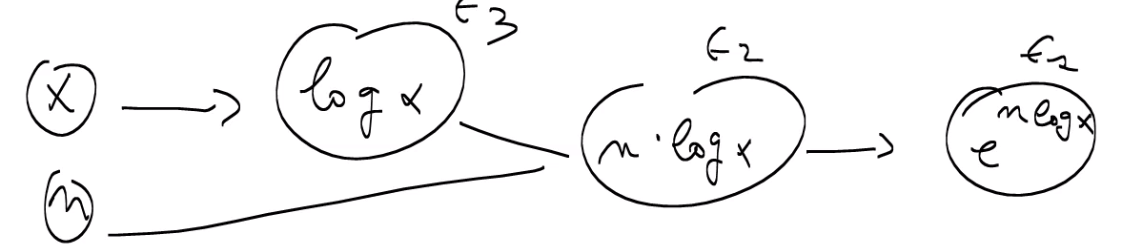
\includegraphics[scale=0.4]{es2_grafo2.png}
\end{center}
$|\epsilon_1| \leq u$, $|\epsilon_2| \leq u$, $|\epsilon_3| \leq u$\\
Per $x \rightarrow \log(x)$ allora $C_x = \frac{\frac{1}{x}}{\log(x)} = \frac{1}{\log(x)}$ ma non amplifica errore su $x$, perché per il calcolo dell'errore algoritmi assumiamo numeri di macchina.\\
Per $x \rightarrow e^x$ allora $C_x = \frac{e^x}{e^x}x = x$. Quindi $\epsilon_2$ ha come coefficiente di amplificazione pari a $n\cdot\log(x)$.\\
Di conseguenza calcolo l'errore algoritmico partendo dalla cima dell'albero e verso le radici (destra verso sinistra) $$\epsilon_{alg} \doteq \epsilon_1 + (n\cdot\log(x))(\epsilon_2 + \epsilon_3)$$
Concludiamo che $|\epsilon_{alg}| = |\epsilon_1 + n\log(x)(\epsilon_2 + \epsilon_3)| \leq |\epsilon_1| + |n\log(x)(\epsilon_2 + \epsilon_3)| \leq u + |n\log(x)|\cdot |\epsilon_2 + \epsilon_3| \leq u + n|\log(x)|(|\epsilon_2| + |\epsilon_3|) \leq u + 2un|\log(x)| = u\cdot(1 + 2\cdot n\cdot|\log(x)|)$ cioè $$|\epsilon_{alg}| \leq u\cdot(1 + 2\cdot n\cdot|\log(x)|)$$ Concludiamo che l'algoritmo è \textbf{numericamente instabile per $x$ piccolo o $x$ è grande}, ma è stabile in un intorno di $1$.\\\\\\\\
L'analisi della stabilità ci dice che il primo algoritmo è preferibile.
\paragraph{Costo computazionale} Il \textbf{primo algoritmo} $\Rightarrow$ $(n - 1)$ operazioni moltiplicative, quindi \textbf{O(n)}.\\
Il \textbf{secondo algoritmo}, più complicato perché ci sono due operazioni non razionali oltre alla moltiplicazione.
\paragraph{Esercizio} Supposto $n = 2^k$ e $f(x) = x^n = x^{2^k}$, determinare un algoritmo che calcola $f(x)$ con $k = \log_2(n)$ operazioni moltiplicative. Eseguire anche l'analisi dell'errore algoritmico per l'algoritmo trovato.
\pagebreak
\paragraph{Esercizio 1}
$A = I + \alpha e e^T$ con $e^T = [1\ldots ]^T$ vettore colonna, quindi $n \times 1$. $e\cdot e^T$ è quindi una matrice $n \times n$.\\
Quindi $A = I + \alpha\left[
\begin{array}{c c c}
	1 & \ldots & 1\\
	 & \ldots\\
	1 & \ldots & 1
\end{array}
\right]
= I + \left[
\begin{array}{c c c}
	\alpha & \ldots & \alpha\\
	 & \ldots\\
	\alpha & \ldots & \alpha
\end{array}
\right]
$
\begin{enumerate}
	\item Per quali valori di $\alpha$, $A$ è invertibile?
	\item Mostrare che l'inversa è $B = I + \beta e e^T$
	\item Analizzare il condizionamento di $A$
\end{enumerate}
\subparagraph{1.} Matrice è singolare $\Leftrightarrow$ $Ax = 0$ ha una soluzione non nulla $\Leftrightarrow \left\{ \begin{array}{l }
	x_1 + \alpha \sum x_i = 0\\
	\vdots\\
	x_n + \alpha \sum x_i = 0
\end{array}
\right.
\Rightarrow x_1 = x_2 = \ldots = x_n = x
$\\
$x + \alpha \sum _{i = 1}^n x_i = x + n \alpha x = x (1 + n\alpha)$\\
Se $1 + n\alpha \neq 0$, $x = 0 \Rightarrow x_1 = \ldots = x_n = 0$\\
Se $1 + n\alpha = 0$, $\alpha = -\frac{1}{n}$\\
$A$ singolare $\Leftrightarrow$ $\alpha = \frac{1}{n}$
\subparagraph{2.} $I = (I + \alpha e e^T)(I + \beta e e^T) \Leftrightarrow I = I + \beta e e^T + \alpha e e^T + \alpha e e^T \beta e e^T$ con $\alpha$, $\beta$ scalari quindi commutano\\
$\not I = \not I + \beta e e^T + \alpha e e^T + \alpha \beta e(e^Te)e^T $ con $e^Te$ scalare $= n \Leftrightarrow 0 = (\beta + \alpha + \alpha \beta n)e e^T$ con $e e^T \neq 0$\\
$\Leftrightarrow \alpha + \beta + \alpha \beta n = 0$\\
$\Leftrightarrow \beta = \frac{-\alpha}{1 + \alpha n}$ con $\alpha \neq -\frac{1}{n}$\\
Quindi l'inversa è $I + \beta e e^T \Leftrightarrow \beta = \frac{-\alpha}{1 + \alpha n}$
\subparagraph{3.} $A = \left[\begin{array}{c c c c}
	\alpha + 1 & \alpha & \ldots & \alpha\\
	\alpha & \alpha + 1 & \alpha\ldots & \alpha\\
	\ldots & & \ldots &
\end{array}
\right]
||A||_\infty\ldots$\\
%TODO
$K_\infty(A) = (|\alpha + 1| + (n - 1)|\alpha|)(|\beta + 1| + (n-1)|\beta|)$\\
Mal condizionato per $|\alpha| \rightarrow +\infty$
%TODO
\paragraph{Esercizio 2} $A = I + \theta e_1 e_n ^T + \theta e_n e_1^T$
%TODO
$A = (a_{ij})$ con $a_{ij} = min(i, j)$
\begin{enumerate}
	\item Dire se A ammette fattorizzazione LU
	\item In caso affermativo, determinare la fattorizzazione
	\item Dire se la fattorizzazione è unica
	\item Mostrare che A è invertibile
	\item Scrivere un programma Matlab per la risoluzione di $Ax = b$ con costo lineare
\end{enumerate}
$A \in \mathbb{R}^{n \times n}$ con $a_{ij} = min(i, j)$\\
Ad esempio $n = 4$, abbiamo
\begin{math}
A = \left[
\begin{array}{c c c c}
	1 & 1 & 1 & 1\\
	1 & 2 & 2 & 2\\
	1 & 2 & 3 & 3\\
	1 & 2 & 3 & 4
\end{array}
\right]
\end{math}
Difficile applicare il teorema, perché valutare la complessità delle sottomatrici principali di testa ha la stessa complessità: sono dello stesso tipo della matrice $A$.\\
Analizziamo i casi minori, $n = 2$ quindi \begin{math}
A = \left[
\begin{array}{c c}
	1 & 1\\
	1 & 2
\end{array}
\right]
= \left[
\begin{array}{c c}
	1 & 0\\
	l & 1
\end{array}
\right]
\left[
\begin{array}{c c}
	u_1 & u_2\\
	0 & u_3
\end{array}
\right]
\end{math}
e avremo $u_1 = 1, u_2 = 1, u_3 = 1$ e $l = 1$\\
Quindi \begin{math}
A = \left[
\begin{array}{c c}
	1 & 1\\
	1 & 2
\end{array}
\right]
= \left[
\begin{array}{c c}
	1 & 0\\
	1 & 1
\end{array}
\right]
\left[
\begin{array}{c c}
	1 & 1\\
	0 & 1
\end{array}
\right]
\end{math}\\
$n = 3$ quindi \begin{math}
A = \left[
\begin{array}{c c c}
	1 & 1 & 1\\
	1 & 2 & 2\\
	1 & 2 & 3
\end{array}
\right]
\end{math}
e usando il teorema, procediamo "upgradando" la fattorizzazione di ordine 2\\
\begin{math}
A = \left[
\begin{array}{c c c}
	1 & 1 & 1\\
	1 & 2 & 2\\
	1 & 2 & 3
\end{array}
\right]
= \left[
\begin{array}{c c | c}
	1 & 0 & 0\\
	1 & 1 & 0\\
	\hline
	 & & 1
\end{array}
\right]
\left[
\begin{array}{c c | c}
	1 & 1 & \\
	0 & 1 & \\
	\hline
	0 & 0 & 
\end{array}
\right]
= \left[
\begin{array}{c c c}
	1 & 0 & 0\\
	1 & 1 & 0\\
	1 & 1 & 1
\end{array}
\right]
\left[
\begin{array}{c c c}
	1 & 1 & 1\\
	0 & 1 & 1\\
	0 & 0 & 1
\end{array}
\right]
\end{math}
Ottenendo di nuovo una triangolare superiore con tutti 1 e una triangolare inferiore con tutti 1. Ma non posso dire che \textit{chiaramente} anche la matrice di ordine $n$ generico si fattorizza così, perché fattorizzare per $n$ non dà alcuna informazione sulla fattorizzazione di $m > n$.\\
Posso \textit{dimostrare} che $A$ si fattorizza LU con due matrici una triangolare inferiore e una triangolare superiore con tutti 1\\
$B = LU = (b_{ij})$ con $b_{ij} = (i$-esima riga di $L)\times(j$-esima colonna di $U) = 1 + 1 + \ldots + 1$ per $min(i, j)$ volte quindi $= min(i, j)$ e quindi $B = A$\\
Quindi ho dimostrato che $A$ si fattorizza LU con due matrici una triangolare inferiore con tutti 1 per una triangolare superiore per tutti 1.\\\\
Invertibile? det$A =$ det$(LU)$ = det$L\cdot$det$U = 1 \cdot 1$ = $1 \neq 0$ quindi $A$ è invertibile.\\
Osservo che $A = L \cdot U$ e il termine della sottomatrice principale di ordine $k$ di $A$, cioè \begin{math}
A = \left[
\begin{array}{c | c}
	A_k & \\
	\hline
	&
\end{array}
\right]
= \left[
\begin{array}{c | c}
	L_k & \\
	\hline
	&
\end{array}
\right]
\left[
\begin{array}{c | c}
	U_k & \\
	\hline
	&
\end{array}
\right]
\end{math}\\
Quindi $A_k = L_k\cdot U_k$ quindi la fattorizzazione LU di A implica una fattorizzazione LU di tutte le radici principali di testa.\\\\
Risoluzione di $Ax = b$, usando la fattorizzazione $LU$ perché $LUx = b$ e $Ux = y$ e $Ly = b$.
\begin{lstlisting}
y(1) = b(1)/l(1, 1);
for k = 2:n
	s = 0;
	for j = 1:k-1
		s = s + l(k, j)*y(j);
	end
	y(k) = (b(k) - s)/l(k ,k);
end
\end{lstlisting}
In generale questo algoritmo ha un costo quadratico. Ma gli elementi di $l$ sono $= 1$
\begin{lstlisting}
y(1) = b(1);
for k = 2:n
	s = 0;
	for j = 1:k-1
		s = s + y(j);
	end
	y(k) = b(k) - s;
end
\end{lstlisting}
Non faccio più operazioni moltiplicative, ma il costo rimane quadratico. Ma posso fare un'osservazione: $s = s + y_j$ è una somma crescente
\begin{lstlisting}
y(1) = b(1);
s = 0
for k = 2:n
	s = s + y(k - 1);
end
\end{lstlisting}
Diventando così a costo lineare O($n$)
\pagebreak
\paragraph{Esercizio 2} 
\begin{math}
A = \left[
\begin{array}{c c c c}
	1 & - \gamma_1 & & \\
	& 1 & \ddots & \\
	& & 1 & -\gamma_{n-1} \\
	\gamma_0 & & & 1\\
\end{array}
\right]
\end{math}
Proviamo che se $|\gamma_i| <$ 1 allora A è invertibile.\\Possiamo farlo con \textbf{Gerschgorin}:
\begin{list}{}{}
	\item $K_i = \{ z \in C\:|\: |z-1| \leq |\gamma_i|\}$ per $i = 1..n-1$
	\item $K_n = \{ z \in C\:|\: |z-1| \leq |\gamma_0|\}$
\end{list}
$$1 - |\gamma_i| > 0 \Leftrightarrow 1 > |\gamma_i| \Leftrightarrow |\gamma_i| < 1$$
$$|\gamma_i| < 1 \Rightarrow 1 - |\gamma_i| > 0 \Rightarrow 0 \not\in K_i \Rightarrow 0 \not\in \bigcup_{i=1}^n K_i \Rightarrow A\textsl{ è invertibile}$$
\subparagraph{Fattorizzazione LU} $A_k = \left[
\begin{array}{c c c c}
	1 & - \gamma_1 & & \\
	& 1 & \ddots & \\
	& & 1 & -\gamma_{k-1}
\end{array}
\right]$\\Triangolare superiore con elementi diagonali $\neq 0 \Rightarrow A_k$ invertibile per $k = 1..n-1 \Rightarrow \exists!\:LU$ di $A$\\
\begin{math}
A = \left[ \begin{array}{c c c | c}
	1 & -\gamma_1 & & \\
	& \ddots & \ddots & \\
	& &\ddots & -\gamma_{n-1}\\
	\hline
	\gamma_0 & & & 1
\end{array} \right] =
\left[ \begin{array}{c c c | c}
	& & & \\
	& & & \\
	& I_{n-1} & & 0 \\
	& & & \\
	& & & \\
	\hline
	x_1 & \ldots & x_{n-1} & 1
\end{array} \right] \cdot
\left[ \begin{array}{c c c c | c}
	1 & -\gamma_1 & & & 0\\
	& \ddots & \ddots & & \vdots\\
	& & \ddots & -\gamma_{n-2} & 0\\
	& & & 1 & -\gamma_{n-1}\\
	\hline
	& & 0^T & & \beta
\end{array} \right]
\end{math}\\
\begin{math}
\left[x_1 \ldots x_n\right]\cdot\left[ \begin{array}{c c c c}
	1 & -\gamma_1 & & \\
	& \ddots & \ddots &  \\
	& & \ddots & -\gamma_{n-2} \\
	& & & 1
\end{array} \right]
= \left[ \gamma_0\: 0 \ldots 0 \right] \rightarrow \left\{
\begin{array}{ll}
x_1 = \gamma_0\\
-x_1\gamma_1 + x_2 = 0 \Leftrightarrow x_2 = \gamma_0\gamma_1\\
-x_2\gamma_2 + x_3 = 0 \Leftrightarrow x_3 = x_2\gamma_2 = \gamma_0\gamma_1\gamma_2\\
\vdots\\
x_{n-1} = \gamma_0\gamma_1\ldots\gamma_{n-1}
\end{array}
\right.
\end{math}\\
\begin{math}
\left[ x_1\ldots x_{n-1} \right]\cdot\left[\begin{array}{c}
 0\\\vdots\\0\\-\gamma_{n-1}
\end{array} \right] + \beta = 1 \Leftrightarrow \beta = 1 + x_{n-1}\gamma_{n-1} = 1 + \gamma_0\gamma_1\ldots\gamma_{n-2}\gamma_{n-1} \Leftrightarrow \mathlarger{ \beta = 1 + \prod_{i=0}^{n-1} \gamma_i}
\end{math}\\
Determiniamo per quali valori di $\gamma_i$ $A$ è invertibile.\\
Sappiamo che $A$ invertibile $\Leftrightarrow \textsl{det}(U) \neq 0 \Leftrightarrow\textsl{det}(U) = \beta \neq 0 \Leftrightarrow \mathlarger{\prod_{i=0}^{n-1} \gamma_i} \neq -1$\\
Se $|\gamma_i| < 1 \Rightarrow\:\vline\:\mathlarger{\prod_{i=0}^{n-1} \gamma_i}\:\vline = \mathlarger{\prod_{i=0}^{n-1} |\gamma_i|} < 1$
\begin{math}
A = \left[ \begin{array}{c c c}
	a & & 1\\
	& \ddots & \\
	1 & & a
\end{array} \right] \in \mathbb{R}^{n \times n}
\end{math}
con $a \in \mathbb{R}$
\paragraph{Per quali $a$, $A$ ammette LU?}  Abbiamo \begin{math}
A_k = \left[ \begin{array}{c c c}
	a & & \\
	& \ddots & \\
	& & a
\end{array} \right] \in \mathbb{R}^{k \times k}
\end{math}
per $k = 1\ldots n-1$\\
$\textsl{det}(A_k) = a^k \neq 0 \Leftrightarrow a \neq 0$, quindi \textbf{$A_k$} per $k = 1\ldots n-1$ \textbf{è invertibile $\Leftrightarrow a \neq 0$}\\
Quindi, per il \textbf{teorema di esistenza ed unicità}, $a \neq 0 \Rightarrow \exists!$ fattorizzazione $LU$ di $A$\\
\begin{math}
A_{n-1} = \left[
\begin{array}{c c c}
	a & & \\
	& \ddots & \\
	& & a
\end{array}
\right] = I_{n-1} \cdot \left[
\begin{array}{c c c}
	a & & \\
	& \ddots & \\
	& & a
\end{array}
\right]
\end{math}\\
\begin{math}
A = \left[ 
\begin{array}{c c c c | c}
 & & & &\\
 & I_{n-1} & & & 0\\
 & & & &\\
 \hline
 \mathlarger{\frac{1}{a}} & 0 & \ldots & 0 & 1
\end{array}
\right] \left[
\begin{array}{c c c c | c}
 a & & & & 1\\
 & \ddots & & & 0\\
 & & & & \vdots \\
 & & & a & 0 \\
 \hline
 & 0^T & & & \mathlarger{a - \frac{1}{a}}
\end{array}
\right]
\end{math}\\
\begin{math}
I_{n-1} \cdot z = \left[ \begin{array}{c} 1\\0\\\vdots\\0\end{array} \right]
\Leftrightarrow
z = \left[ \begin{array}{c} 1\\0\\\vdots\\0\end{array} \right]
\end{math}\\
\begin{math}
x^T\cdot\left[
\begin{array}{c c c}
	a & & \\
	& \ddots & \\
	& & a
\end{array}
\right] = [1\:0\ldots0] \Rightarrow \left\{ \begin{array}{l}
x_1a = 1\\x_2a = 0\\\vdots\\a_{n-1}a = 0
\end{array} \right. \Leftrightarrow \left\{ \begin{array}{l}
x_1 = \mathlarger{\frac{1}{a}}\\x_2 = x_3 = \ldots = x_{n-1} = 0
\end{array} \right.
\end{math}\\
\begin{math}
\mathlarger{\frac{1}{a}} + \beta = a \Leftrightarrow \mathlarger{\beta = a - \frac{1}{a}}
\end{math}
\paragraph{Dimostrare che $A$ è invertibile per $|a| > 1$} Usiamo \textbf{Gerschgorin}
\begin{list}{}{Per $a > 0$}
	\item $K_1 = K_n = \{z \in C\:|\: |z - a| \leq 1\}$
	\item $K_2 = \ldots = K_{n-1} = \{z \in C\:|\:|z - a| = 0\}$
\end{list}
Per $a > 1 \Leftrightarrow a - 1 > 0$ ottengo $0 \not\in \bigcup K_i$\\
$\Rightarrow$ A è invertibile per $a > 1$\\
Per $a < 0 \Rightarrow a < -1 \Leftrightarrow a + 1 < 0 \Rightarrow 0 \not\in\bigcup K_i$\\
$\Rightarrow$ A è invertibile per $a < -1$\\
$\Rightarrow$ \textbf{A invertibile} per $|a| > 1$
\paragraph{Determinante di A} Usiamo \textbf{Laplace}\\
$A = LU \Rightarrow \textsl{det}(A) = \textsl{det}(L)\cdot\textsl{det}(U)$ (per \textbf{Binet})\\
$\textsl{det}(U) = \mathlarger{\prod_{k=1}^n u_{kk}} = a^{n-1}(a - \frac{1}{a}) = a^n - a^{n-2} = a^{n-2}(a^2 - 1)$\\
A è singolare $\Leftrightarrow$ U è singolare $\Leftrightarrow a = 0 \vee a = \pm 1 $
\paragraph{} $f(a) = a^n - a^{n-2}$\\
$C_a = \mathlarger{\frac{f'(a)}{f(a)}\cdot a}$\\
$|\epsilon_{in}| = |C_a|\cdot|\epsilon_a| \leq |C_a|a$
$$C_a = \frac{n\cdot a^{n-1} - (n-2)\cdot a^{n-3}}{a^n - a^{n-2}}\cdot a$$
$$C_a = \frac{\not a^{n-2}(n\cdot a^2 - (n-2))}{\not a^{n-2}(a^2 - 1)}$$
$$C_a = \frac{n\cdot a^2 - (n-2)}{a^2 - 1}$$
\textbf{Mal condizionato per $a\to\pm1$}\\
Cosa posso dire quando $|a| \to +\infty$? $a^2\to+\infty$\\
$$\lim_{|a|\to+\infty} C_a = \lim_{|a|\to+\infty} \frac{n\cdot a^2 - (n-2)}{a^2 - 1} = \lim_{|a|\to+\infty} \frac{\not a^2(n - \frac{n-2}{a^2})}{\not a^2(1 - \frac{1}{a^2})} = n$$
Quindi è \textbf{ben condizionato per $|a|\to+\infty$}
\begin{math}
A = \left[ 
\begin{array}{c c c c}
1 & \theta & \ldots & \theta \\
-\theta & \ddots & &\\
\vdots & & \ddots &\\
-\theta & & & 1
\end{array}
\right]
\:\:\:\:\textsl{con }\theta\in \mathbb{R}
\end{math}
\paragraph{Determinare condizioni sufficienti su $\theta$ affinché $A$ abbia fattorizzazione $LU$} Predominanza diagonale
\begin{list}{}{}
	\item[$i = 1 \rightarrow$] $|1| = 1 > (n-1)|\theta| \Leftrightarrow |\theta| < \mathlarger{\frac{1}{n-1}}$\\
$\Leftrightarrow \mathlarger{-\frac{1}{n-1} < \theta < \frac{1}{n-1}}$
\item[$i = 2\ldots n \rightarrow$] $|1| = 1 > |-\theta| = |\theta| \Leftrightarrow |\theta| < 1$\\ 
$\Leftrightarrow -1 < \theta < 1 $
\end{list}
Quindi $A$ è predominante diagonale $\Leftrightarrow \mathlarger{-\frac{1}{n-1} < \theta < \frac{1}{n-1}} \Rightarrow \exists!\: \text{ la fattorizzazione }LU$
\paragraph{Determinare tutti i valori di $\theta$ per i quali A ammette fattorizzazione $LU$} Determinante?\\$\textsl{det}(\left[ 
\begin{array}{c c c c}
1 & \theta & \ldots & \theta \\
-\theta & \ddots & &\\
\vdots & & \ddots &\\
-\theta & & & 1
\end{array}
\right]) = \textsl{det}(\left[ 
\begin{array}{c c c c}
1 & & & -\theta\\
& \ddots & & \vdots\\
& & \ddots & -\theta\\
\theta & \ldots & \theta & 1
\end{array}
\right])$\\
Questo perché passo da $\left[ 
\begin{array}{c c c c}
1 & \theta & \ldots & \theta \\
-\theta & \ddots & &\\
\vdots & & \ddots &\\
-\theta & & & 1
\end{array}
\right]$ a $\left[ 
\begin{array}{c c c c}
1 & & & -\theta\\
& \ddots & & \vdots\\
& & \ddots & -\theta\\
\theta & \ldots & \theta & 1
\end{array}
\right]$ semplicemente scambiando righe e colonne.\\
Questa osservazione è utile perché di $\left[ 
\begin{array}{c c c c}
1 & \theta & \ldots & \theta \\
-\theta & \ddots & &\\
\vdots & & \ddots &\\
-\theta & & & 1
\end{array}
\right]$ a $\left[ 
\begin{array}{c c c c}
1 & & & -\theta\\
& \ddots & & \vdots\\
& & \ddots & -\theta\\
\theta & \ldots & \theta & 1
\end{array}
\right]$ so calcolare la fattorizzazione $LU$.
$$\left[ \begin{array}{c c c | c}
  & & & \\
  & I_{n-1} & & \\
  & & & \\
  \hline
  \theta &\ldots &\theta & 1
\end{array}\right] \cdot \left[ \begin{array}{c c c | c}
  & & & -\theta\\
  & I_{n-1} & &\vdots \\
  & & &-\theta \\
  \hline
  & 0 & & 1 + (n-1)\theta^2
\end{array}\right]$$
Questo mi dice che $\textsl{det}(A) = 1 + (n-1)\theta^2 \neq 0\:\:\forall\:\theta$\\
Quindi le sottomatrici principali di testa sono invertibili $\forall\:\theta$, quindi \textbf{ammette unica fattorizzazione $LU$ $\forall\:\theta$}
\paragraph{Determinare $E_1$ matrice elementare di Gauss tale che $E_1\cdot A$ abbia 0 nella prima colonna esclusa la prima posizione} $E_1 = ?$, ricordando la costruzione della matrice di Gauss ottengo
$$E_1 = \left[ \begin{array}{c c c c}
1\\
+\theta & \ddots\\
\vdots & & \ddots\\
+\theta & & & 1
\end{array} \right]$$
$$E_1 A = \left[ \begin{array}{c c c c}
1\\
+\theta & \ddots\\
\vdots & & \ddots\\
+\theta & & & 1
\end{array} \right]\cdot\left[ 
\begin{array}{c c c c}
1 & \theta & \ldots & \theta \\
-\theta & \ddots & &\\
\vdots & & \ddots &\\
-\theta & & & 1
\end{array}
\right] = \left[ 
\begin{array}{c c c c c c }
1 & \theta & \ldots & \ldots & \ldots & \theta \\
0 & 1 + \theta^2 & \theta^2 & \ldots & \ldots & \theta^2\\
\vdots & \theta^2 & 1 + \theta^2 & \theta^2 & \ldots & \theta^2\\
\vdots & \vdots & &\ddots & & \vdots\\
\vdots & \vdots & & & \ddots & \theta^2\\
0 & \theta^2 & \ldots & \ldots & \theta^2 & 1 + \theta^2
\end{array}
\right]$$
Con $1 + \theta^2$ sulla diagonale principale e $\theta^2$ fuori da essa.\\
Notiamo che $A$ è una matrice sparsa, cioè \textit{tanti elementi di $A$ sono $0$}, che è una proprietà che vogliamo sfruttare. Ma in generale \textbf{il metodo di eliminazione gaussiana non preserva la sparsità della matrice}. Si riempiono sia $A^{(k)}$ sia $L$ e $U$: questo si chiama \textbf{fill-in}.
\pagebreak
\paragraph{Esercizio}
\begin{multicols}{2}
\begin{center}
	$$A = \left[\begin{array}{c c c c}
	2 + h & -1\\
	-1 & \ddots & \ddots\\
	& \ddots & \ddots & -1\\
	& & -1 & 2+h
\end{array}\right]$$
\end{center}
\columnbreak
\begin{enumerate}
	\item Determinare condizioni sufficienti su $h$ tali da garantire esistenza ed unicità della fattorizzazione $LU$
	\item Sotto tali condizioni, scrivere un programma per il calcolo dei fattori $L$ e $U$
\end{enumerate}
\end{multicols}
\begin{enumerate}
	\item Proviamo attraverso la predominanza diagonale
	\begin{list}{}{}
		\item[$i = 1$, $n \rightarrow$] $|2+h| > 1$
		\item[$i = 2\ldots n-1 \rightarrow$] $|2+h| > 2$
	\end{list}
	Quindi la condizione sarà $|2+h| > 2 \Leftrightarrow \left\{\begin{array}{l}
	2 + h > 2\\
	2 + h \geq 0
	\end{array}\right. \bigcup \left\{\begin{array}{l}
	-(2 + h) > 2\\
	2 + h \leq 0
	\end{array}\right. \Leftrightarrow \left\{\begin{array}{l}
	h > 0\\
	h \geq -2
	\end{array}\right. \bigcup \left\{\begin{array}{l}
	h < -4\\
	h \leq -2
	\end{array}\right.$\\
	$\Rightarrow$ la matrice è predominante diagonale quando $h < -4 \vee h > 0$
	\item Abbiamo le condizioni, vediamo come si comportano $L$ ed $U$\\
	Abbiamo una matrice del tipo $\left[\begin{array}{c c c c}
	a & b\\
	b & \ddots & \ddots\\
	& \ddots & \ddots & b\\
	& & b & a
\end{array}\right]$ con $a = 2+h$ e $b = -1$. Il primo passo della fattorizzazione è mettere $0$ nella prima colonna. L'unico elemento da annullare è quello in posizione $(2, 1)$, basta quindi prendere $\mathlarger{-\frac{b}{a}}$ come elemento corrispondente in $E_1$
$$E_1 = \left[\begin{array}{c c c}
1 & & \\
\mathlarger{-\frac{b}{a}} & \ddots\\
& & 1
\end{array} \right]$$
$$E_1 A = \left[\begin{array}{c c c c c}
a & b & &\\
0 & \overline{a} & b & \\
\vdots & b & a & \ddots\\
0 & & \ddots & \ddots
\end{array} \right]$$
La matrice su cui dovrò lavorare, cioè $E_1 A$ privata della prima riga e della prima colonna, è ancora tridiagonale. In questo caso, e in generale nelle matrici cosiddette "a banda", il metodo di eliminazione gaussiama preserva la sparsità.\\
$E_2$ sarà analogamente con un elemento $\mathlarger{-\frac{b}{a}}$\ldots\\
La $U$ sarà una bidiagonale superiore, mentre la $L$ sarà bidiagonale inferiore.
\end{enumerate}
\paragraph{Esempio} \begin{multicols}{2}
$$A = \left[\begin{array}{c c c c}
\alpha & 1 & & 0\\
\vdots & \ddots & \ddots\\
\vdots & & \ddots & 1\\
\alpha & \ldots & \ldots & \alpha
\end{array} \right] \in\mathbb{R}^{n\times n}\text{ con }n\geq 2$$
\paragraph{Predominante diagonale?}
\begin{list}{}{}
	\item[$i = 1 \rightarrow$] $|a| > 1$
	\item[$i = 2 \rightarrow$] $\left\{\begin{array}{l l}
	n = 2 & |a| > |a|\\
	n > 2 & |a| > |a| + 1
	\end{array}\right.$
\end{list}
Quindi non è predominante diagonale per nessun valore $\alpha$
\end{multicols}
\paragraph{Per quali $\alpha$, G-S converge?}
$$M = \left[\begin{array}{c c c c}
\alpha &  & & \\
\vdots & \ddots & 0 \\
\vdots & & \ddots & \\
\alpha & \ldots & \ldots & \alpha
\end{array} \right]\:\:\:\:\:\:\:\:N = \left[\begin{array}{c c c c}
& -1 & & 0\\
& & \ddots\\
& 0 & & -1\\
& &  & 
\end{array} \right]$$
Devo studiare $\rho(G) = \textsl{max}_{i=1}^n |\lambda_i|$ \\
$G = \left[\begin{array}{c c c c}
\alpha &  & & \\
\vdots & \ddots & 0 \\
\vdots & & \ddots & \\
\alpha & \ldots & \ldots & \alpha
\end{array} \right]^{-1}\cdot\left[\begin{array}{c c c c}
& -1 & & 0\\
& & \ddots\\
& 0 & & -1\\
& &  & 
\end{array} \right]$
\begin{list}{}{}
	\item $\left(\alpha\cdot\left[\begin{array}{c c c c}
1 &  & & \\
\vdots & \ddots & 0 \\
\vdots & & \ddots & \\
1 & \ldots & \ldots & 1
\end{array} \right]\right)^{-1} = \mathlarger{\frac{1}{\alpha}}\cdot\left[\begin{array}{c c c c}
1 &  & & \\
\vdots & \ddots & 0 \\
\vdots & & \ddots & \\
1 & \ldots & \ldots & 1
\end{array} \right]^{-1}$
	\item Sapendo che $\left[\begin{array}{c c c c}
		1\\
		1&1\\
		1&1&1\\
		1&1&1&1
	\end{array}\right]\cdot\left[\begin{array}{c c c c}
		1\\
		-1&1\\
		0&-1&1\\
		0&0&-1&1
	\end{array}\right] = \left[\begin{array}{c c c c}
		1\\
		&1\\
		& &1\\
		& & &1
	\end{array}\right]$, allora ipotizzo che\\
	$\left[\begin{array}{c c c c}
1 &  & & \\
\vdots & \ddots & 0\\
\vdots & & \ddots & \\
1 & \ldots & \ldots & 1
\end{array} \right]\cdot\left[\begin{array}{c c c c}
1 &  & & \\
-1 & \ddots &0 \\
 & \ddots & \ddots & \\
 0&  & -1 & 1
\end{array} \right] = \left[\begin{array}{c c c c}
		1\\
		&\ddots & 0\\
		&0&\ddots\\
		& & &1
	\end{array}\right]$
\end{list}
$M^{-1} = \mathlarger{\frac{1}{\alpha}}\left[\begin{array}{c c c c}
1 &  & & \\
-1 & \ddots &0 \\
 & \ddots & \ddots & \\
 0&  & -1 & 1
\end{array} \right]$
$$G = M^{-1}N = \mathlarger{\frac{1}{\alpha}}\left[\begin{array}{c c c c}
1 &  & & \\
-1 & \ddots &0 \\
 & \ddots & \ddots & \\
 0&  & -1 & 1
\end{array} \right]\cdot\left[\begin{array}{c c c c}
& -1 & & 0\\
& & \ddots\\
& 0 & & -1\\
& &  & 
\end{array} \right]
= \mathlarger{\frac{1}{\alpha}}\left[\begin{array}{c c c c c c c}
0 & -1 & 0 & \ldots & \ldots & 0\\
0 & 1 & -1 & 0 & \ldots & 0\\
0 & 0 & 1 & -1 & \ldots & \ldots\\
& & & \ddots & \ddots\\
\\
\\
\end{array} \right] = \left[\begin{array}{c c c c}
0 & -\frac{1}{\alpha} \\
0 & \frac{1}{\alpha} & \ddots\\
& & \ddots & -\frac{1}{\alpha}\\
& & & \frac{1}{\alpha}
\end{array} \right]$$
$G$ triangolare superiore $\Rightarrow$ gli autovalori stanno sulla diagonale principale e sono $\begin{array}{l}
\lambda = 0\\
\lambda = \mathlarger{\frac{1}{\alpha}}
\end{array} \Rightarrow \rho(G) = \mathlarger{\frac{1}{|\alpha|}}$\\
Quindi $\mathlarger{\frac{1}{|\alpha|}} < 1 \Leftrightarrow 1 < |\alpha| \Leftrightarrow |\alpha| > 1$\\
$\textsl{det}(\lambda I - M^{-1}N) = \textsl{det}(\lambda M^{-1}M - M^{-1}N) = \textsl{det}(M^{-1}\cdot(\lambda M - N)) =$ (per Binet) $\textsl{det}(M^{-1})\cdot\textsl{det}(\lambda M - N)$\\
Quindi $\textsl{det}(\lambda I - G) = 0 \Leftrightarrow \textsl{det}(\lambda M - N) = 0$
$$\textsl{det}\left(\alpha\lambda\left[\begin{array}{c c c c}
1 &  & & \\
\vdots & \ddots & 0\\
\vdots & & \ddots & \\
1 & \ldots & \ldots & 1
\end{array}\right] + \left[\begin{array}{c c c c}
 & 1 & & \\
 &  &\ddots   \\
 & &  & 1 \\
 &  &  & 
\end{array}\right]\right) = \textsl{det}\left(\left[\begin{array}{c c c c}
\alpha\lambda & 1  & & \\
\vdots & \ddots & \ddots\\
\vdots & & \ddots & 1\\
\alpha\lambda & \ldots & \ldots & \alpha\lambda
\end{array}\right]\right)$$
$M = \left[\begin{array}{c c c}
\alpha\\
\vdots & \ddots\\
\alpha & \ldots & \alpha
\end{array}\right] \Rightarrow \textsl{det}(M^{-1}N) = \textsl{det}(M^{-1})\cdot\textsl{det}(N) = \mathlarger{\frac{\textsl{det}(N)}{\textsl{det}(M)}} = \mathlarger{\frac{\textsl{det}(N)}{\alpha^n}} = \mathlarger{\frac{0}{\alpha^n}} = 0$
%TODO esercitazione 6/5
\pagebreak
\paragraph{Esercizio} $f(x) = \log(e^x + 1) + x - 1 = 0$
\begin{enumerate}
	\item Determina il numero di soluzioni dell'equazione e localizzale\\
	$e^x + 1 > 0\:\:\:\:\forall\:x\Rightarrow f:\mathbb{R}\rightarrow\mathbb{R}$\\
	$\mathlarger{\lim_{x\to\pm\infty}}f(x) = \pm\infty$\\
	$f'(x) = \mathlarger{\frac{1}{e^x + 1}e^x + 1} = \mathlarger{\frac{e^x}{e^x + 1}}+1 > 0\:\:\:\:\forall\:x\in\mathbb{R}$\\
	$f''(x) = \mathlarger{\frac{e^x\cdot(e^x + 1) - e^x\cdot e^x}{(e^x + 1)^2}} = \mathlarger{\frac{e^x}{(e^2 + 1)^2}} > 0\:\:\:\:\forall\:x\in\mathbb{R}$\\
	$\Rightarrow f \in C^2(\mathbb{R})$, $f(0) = \log 2 - 1 < 0$\\
	Quindi è sempre crescente e negativa a sinistra di $\alpha\:|\:f(\alpha) = 0$, positiva a destra.\\
	$f(1) = \log(e + 1) > 0 \Rightarrow \alpha\in[0, 1]$ \textbf{intervallo di separazione}.
	\item Studia la convergenza $x_{k+1} = 1 - \log(e^{x_k} + 1)$ con $k \geq 0$\\
	Cioè $x_{k+1} = g(x_k)$ con $g(x) = 1 - \log(e^x + 1)$\\
	$\log(e^x + 1) + x - 1 = 0 \Leftrightarrow x = 1 - \log(e^x + 1)$\\
	$g \in C^1(\mathbb{R})$, $|g'(x)| =\:\vline\mathlarger{-\frac{e^x}{e^x + 1}}\:\vline = \mathlarger{\frac{e^x}{e^x + 1}}$\\
	$\forall\:x\in\mathbb{R}\:\:\:\:\mathlarger{\frac{e^x}{e^x + 1}} = |g'(x)| < 1$ questo perché $\mathlarger{\frac{e^x}{e^x + 1}} < 1 \Leftrightarrow e^x < e^x + 1 \Leftrightarrow 0 < 1$ vero $\forall\:x$\\
	Quindi $\forall\:x_0\in\mathbb{R}\:\:\:\:x_k \longrightarrow \alpha$
	\item Studia la convergenza del metodo delle tangenti\\
	$x_{k+1} = x_k - \mathlarger{\frac{f(x_k)}{f'(x_k)}} = g(x_k) \Rightarrow g(x_k) = x_k - \mathlarger{\frac{f(x_k)}{f'(x_k)}}$\\
	$f'(x) \neq 0\:\:\:\:\forall\:x \Rightarrow f'(\alpha) \neq 0 \Rightarrow$ convergenza locale\\
	$f(x)f''(x) > 0$\\\\
	$x_1 - \alpha = g(x_0) - g(\alpha) = g'(\xi)\cdot(x_0 - \alpha) = \mathlarger{\frac{f(\xi)f''(\xi)}{(f'(\xi))^2}}\cdot(x_0 - \alpha)$\\
	$x_1 - \alpha \geq 0 \Leftrightarrow x_1 \geq \alpha$\\
	Quindi $\forall\:x_0\geq\alpha$ ho $x_k \longrightarrow \alpha$
\end{enumerate}
\paragraph{Esercizio} $f(x) = \sqrt{x^3} - 3x + 1 = 0$\\
$x^3 \geq 0 \Leftrightarrow x \geq 0$
\begin{list}{}{}
	\item[$x\geq0\:\rightarrow$] $\sqrt{x^3} - 3x + 1 = 0 \Leftrightarrow \sqrt{x^3} = 3x - 1$\\
	$3x - 1 \geq 0 \Leftrightarrow 3x \geq 1 \Leftrightarrow x \geq \mathlarger{\frac{1}{3}}$\\
	$\Leftrightarrow x^3 = (3x - 1)^2$ e $x \geq \mathlarger{\frac{1}{3}} \Leftrightarrow \sqrt{x} = -2$, $x = 4$
\end{list}
$f(x) = \sqrt{x^3} - 3x + 1 = x^{\frac{3}{2}} - 3x + 1$, sempre in $x\geq 0$\\
$\mathlarger{\lim_{x\to+\infty}} f(x) = \mathlarger{\lim_{x\to+\infty}}x^{\frac{3}{2}}(1 - 3x^{-\frac{1}{2}} + x^{-\frac{3}{2}}) = +\infty$\\
$\mathlarger{\lim_{x\to 0^+}} f(x) = f(0) = 1$\\
$f'(x) = \mathlarger{\frac{3}{2}x^{\frac{3}{2} - 1} - 3} = \mathlarger{\frac{3}{2}\sqrt{x} - 3} = \mathlarger{\frac{3}{2}\left(\sqrt{x} - 2 \right)} \geq 0 \Leftrightarrow \sqrt{x} - 2 \geq 0 \Leftrightarrow \sqrt{x} \geq 2 \Leftrightarrow x \geq 4$\\
Quindi da 0 a 4 incluso è decrescente, da 4 in poi è crescente.\\\\
$f''(x) = \mathlarger{\frac{3}{2}\cdot\frac{1}{2} x^{\frac{1}{2} - 1}} = \mathlarger{\frac{3}{4}\cdot\frac{1}{\sqrt{x}}} \geq 0\:\:\:\:\forall\:x\in\mathbb{R}^+$\\
$\Rightarrow f\in C^2(\mathbb{R}^+)$, definita su $x\geq 0$, $C^2$ per $x > 0$\\\\
Convergenza locale ok ($f'(\alpha) \neq 0$, $f'(\beta) \neq 0$), $\alpha\in[0, 4]$ e $\beta\in[4, 9]$\\
$f(4) = \sqrt{2^6} - 12 + 1 = -3$\\
$x_0 \geq \beta$ allora $x_k \longrightarrow \beta$, $4 \leq x_0 \leq \beta$, $x_1 \geq \beta$ allora $x_k \longrightarrow \beta$\\
$0 < x_0 \leq \alpha$ allora $x_k \longrightarrow \alpha$, $\alpha \leq x_0 \leq 4$ allora $x_k \longrightarrow \alpha$
\pagebreak
\paragraph{Esercizio} $f(x) = e^{x^2-1} + x - 1 = 0$
\begin{multicols}{2}
$f \in C^\infty(\mathbb{R})$
\begin{list}{}{}
	\item $\mathlarger{\lim_{x\to+\infty}} e^{x^2-1} + x - 1 = +\infty$
	\item $\mathlarger{\lim_{x\to-\infty}} e^{x^2-1} + x - 1 =$
	\begin{list}{}{}
		\item $e^{x^2 - 1}\rightarrow+\infty$
		\item $x\rightarrow+\infty$
	\end{list}
	$= \mathlarger{\lim_{x\to-\infty}}e^{x^2 - 1}\cdot\mathlarger{\left(1 + \frac{x}{e^{x^2 - 1}} - \frac{1}{e^{x^2 - 1}} \right)} = +\infty$
\end{list}
$f'(x) = e^{x^2 - 1}\cdot 2x + 1$, $f'(x) > 0\:\:\forall\:x\geq 0$
\begin{list}{}{}
	\item[$x < 0 \rightarrow$] $e^{x^2 - 1}\cdot 2x + 1 \geq 0 \Leftrightarrow$\\
	$e^{x^2-1}2x\geq -1 \Leftrightarrow e^{x^2 - 1}\leq \mathlarger{-\frac{1}{2x}}$
\end{list}
$f$ decrescente fino ad $\alpha < 0$, crescente dopo.\\$\alpha$ minimo della funzione. $f(\alpha) =\:?$\\
$f''(x) = e^{x^2-1}4x^2 + e^{x^2-1}2 = e^{x^2-1}\cdot(4x^2 + 2) > 0\:\:\forall\:x\in\mathbb{R}$\\
$f(0) = e^{-1} + 0 - 1 = \mathlarger{\frac{1}{e}}-1 < 0$\\
$f>0, f''>', f'\neq 0$ ok
\begin{list}{}{}
	\item $f(1) = e^0 + 1 - 1 = 1$
	\item $f(-1) = e^0 - 1 - 1 = -1$
	\item $f(-2) = e^{4-1} - 2 - 1 = e^3 - 3 > 0$
\end{list}
Quindi ho $\beta \in [0, 1]$ e $\gamma\in[-2, 0]$ con $f(\beta) = f(\gamma) = 0$\\\\
Per $x_0\geq\beta$ ho $x_k \rightarrow \beta$ per il th. di convergenza in grande.\\
Per $\alpha < x_0 \leq \beta\Rightarrow x_1\geq\beta$ quindi $x_k \rightarrow\beta$\\
Per $x_0\leq \gamma$ ho $x_k \rightarrow \gamma$ per il th. di convergenza in grande.\\
Per $\gamma\leq x_0 < \alpha \Rightarrow x_1 \leq \gamma$ quindi $x_k\rightarrow\gamma$
\end{multicols}
\paragraph{Esercizio} $B = \left[\begin{array}{c c c}
1 & & 1\\
\vdots & \ddots & \vdots\\
1 & \ldots & 1
\end{array} \right] + \left[\begin{array}{c}
0\\\vdots\\0\\1
\end{array}\right]\cdot\left[\begin{array}{c c c c}
0&\ldots&0&1
\end{array}\right] =  \left[\begin{array}{c c c c}
1 & & & 1\\
\vdots & \ddots & & \vdots\\
\vdots & & 1 & 1\\
1 & \ldots & 1 & 2
\end{array} \right]$\\
$B$ invertibile $\Leftrightarrow \textsl{det}(B) \neq 0$. Proviamo a calcolare una fattorizzazione LU, ricordando che una matrice triangolare inferiore con elementi $=1$ sulla diagonale principale si fattorizza come sé stessa per l'identità.\\
$B = \left[\begin{array}{c c c | c}
1 & & & \\
\vdots & \ddots & & 0 \\
1 & \ldots & 1 & \\
\hline
1 & \ldots & 1 & 1
\end{array} \right]\left[\begin{array}{c c c | c}
 & & & v_1\\
 & I_{n-1} & & \vdots \\
 &  &  & v_{n-1} \\
\hline
 & & & v_n
\end{array} \right]$ e devo avere $\left[\begin{array}{c c c}
1 & & \\
\vdots & \ddots &\\
1 & \ldots & 1
\end{array} \right]\cdot\left[\begin{array}{c}
v_1\\\vdots\\v_{n-1}
\end{array} \right] = \left[\begin{array}{c}
1\\\vdots\\1
\end{array} \right]\\\Rightarrow \left\{\begin{array}{l}
v_1 = 1\\
v_2 + v_1 = 1 \Rightarrow v_2 = 0\\
v_3 + v_2 + v_1 = 1 \Rightarrow v_3 = 0
\end{array} \right.$ ottenendo $\left[\begin{array}{c}
v_1 = 1\\v_2 = 0\\\vdots\\v_{n-1} = 0
\end{array} \right]$ da cui traggo (ultima riga di L per ultima colonna di U) $1 + v_n = 2 \Leftrightarrow v_n = 1$ ottenendo la fattorizzazione $$B = \left[\begin{array}{c c c | c}
1 & & & \\
\vdots & \ddots & & 0 \\
1 & \ldots & 1 & \\
\hline
1 & \ldots & 1 & 1
\end{array} \right]\left[\begin{array}{c c c | c}
 & & & 1\\
 & & & 0\\
 & I_{n-1} & & \vdots \\
 &  &  & 0 \\
\hline
 & & & 1
\end{array} \right]$$
$\textsl{det}(B) = \textsl{det}(U) = 1$, quindi $B$ è invertibile.
\paragraph{Esercizio} $f(x) = (x-1)e^{x+1} - a = 0$ con $a > 0$\\
$f\in C^\infty(\mathbb{R})$
\begin{list}{}{}
	\item $\mathlarger{\lim_{x\to+\infty}} (x-1)e^{x+1} - a = +\infty$
	\item $\mathlarger{\lim_{x\to-\infty}} (x-1)e^{x+1} - a = -a$\\
	Questo perché $\mathlarger{\lim_{x\to-\infty}} (x-1)e^{x+1} = \mathlarger{\lim_{x\to-\infty} \frac{x-1}{e^{-x-1}}} = \mathlarger{\lim_{x\to-\infty} \frac{1}{-e^{-x-1}}} = 0$
\end{list}
$f'(x) = e^{x+1} + (x-1)e^{x+1} = e^{x+1}\cdot(1 + x - 1) = xe^{x+1}$, quindi decrescente fino a 0 e crescente da 0.\\
$f''(x) = e^{x+1} + xe^{x+1} = e^{x+1}(1+x)$\\
Ho $f(0) = -e -a$, e un asintoto orizzontale $= -a$ verso sinistra. Quindi se $f(\xi) = 0$ allora $\forall\:x_0>0$ ho $x_k \rightarrow \xi$
\chapter{Matlab}
11 bit esponente rappresentato in traslazione, 52 bit mantissa (53 cifre rappresentabili per il bit nascosto) $\Rightarrow$ $u = B^{1-t} = 2^{-52}$
\section{Esponenziale}
$f(x) = e^x$ approssimato con Taylor $$e^x \simeq 1 + x + \frac{x^2}{2} + \frac{x^3}{3!} + \ldots + \frac{x^n}{n!}$$ Implementiamo un algoritmo che dati $x$, $n$ in input restituisce $y = 1 + x + \frac{x^2}{2} + \frac{x^3}{3!} + \ldots + \frac{x^n}{n!}$ in output.\\
Potrebbe essere utile un programma del tipo
\begin{lstlisting}
y = 1;
for k = 1 .. n
	y = y + x^(k)/factorial(k)
end
\end{lstlisting}
Dal punto di vista del costo computazionale, però, ci sono dei problemi. Al passo $k$ faccio $k$ prodotti per $x^k$ e $k$ prodotti per $k!$, quindi \textbf{circa $2k$ prodotti}.\\
Il costo totale è del tipo $C = 2 + 2\cdot 2 + 2\cdot 3 + \ldots + 2\cdot n = 2(1 + 2 + 3 + \ldots + n)$.\\
Ricordiamo $1 + 2 + \ldots + n = \frac{n(n + 1)}{2}$, quindi $C = \not 2\cdot\frac{n(n+1)}{\not 2} =$ O($n^2$) quindi costo quadratico.\\
Una variazione più efficiente
\begin{lstlisting}
y = 1; p = 1; m = 1;
for k = 1 .. n
	p = p * x;	% accumula le potenze
	m = m * k;	% accumula il fattoriale
	y = y + p/m	% accumula la somma
end
\end{lstlisting}
Al passo $k$ ho 4 operazioni aritmetiche (o 3 operazioni moltiplicative, perché alcune volte si afferma che $t_* >> t_+$ in termini di operazioni tra bit (\textbf{costo booleano}))\\
Il costo totale $C = 4n$ operazioni (o $3n$).\\
I due algoritmi possono produrre numeri molto grandi. Una versione che argina questo problema è la seguente.
\begin{lstlisting}
y = 1; z = 1;
for k = 1 .. n
	z = z * x/k;	% controllare l'esplosione dei numeri
	y = y + z;
end
\end{lstlisting}
\begin{center}
\pagebreak
\textbf{Codice MatLab} (file: \texttt{myexp.m})
\begin{lstlisting}
function [y] = myexp(x,n)
    % y = 1 + x + (x^2)/2 + ... + (x^n)/(n!)
    y = 1; z = 1;
    for k = 1:n
        z = z * x/k;
        y = y + z;
    end
end
\end{lstlisting}
\end{center}
\end{document}
